%% ----------------------------------------------------------------
%% Thesis.tex -- MAIN FILE (the one that you compile with LaTeX)
%% ---------------------------------------------------------------- 

% Set up the document
\documentclass[a4paper, 11pt, oneside]{Thesis}  % Use the "Thesis" style, based on the ECS Thesis style by Steve Gunn
\graphicspath{Figures/}  % Location of the graphics files (set up for graphics to be in PDF format)

% Include any extra LaTeX packages required
\usepackage[square, numbers, comma, sort&compress]{natbib}  % Use the "Natbib" style for the references in the Bibliography
\usepackage{verbatim}  % Needed for the "comment" environment to make LaTeX comments
\usepackage{vector}  % Allows "\bvec{}" and "\buvec{}" for "blackboard" style bold vectors in maths
\hypersetup{urlcolor=blue, colorlinks=true}  % Colours hyperlinks in blue, but this can be distracting if there are many links.
\usepackage{url}
\usepackage{pdfpages}
\usepackage{hyperref}
\newcommand\fnurl[2]{
	\footnote{\href{#2}{#1} - {#2}}
}
\usepackage{rotating}
\usepackage{enumitem}
\setlist{nolistsep}
\usepackage{fancyhdr}
\renewcommand{\chaptermark}[1]{%
	\markboth{\chaptername
	\ \thechapter.\ #1}{}
}


%% SHORTCUTS ------------------------------------------------------
\newcommand{\rpi}{Raspberry Pi}
\newcommand{\buddy}{AsthmaBuddy}
\newcommand{\iref}{ \emph{INSERT REFERENCE }}
\newcommand{\etal}{et. al.}

%% ----------------------------------------------------------------
\begin{document}
\frontmatter      % Begin Roman style (i, ii, iii, iv...) page numbering
\setlist[enumerate]{itemsep=2mm}

% Set up the Title Page
\title  {Using Mobile Technology to Treat Asthmatic Children}
\authors  {Esben Aarseth and Aleksander Gisvold \\
		Supervisor: Pieter Jelle Toussaint \\
		Co-Supervisors: Ole Andreas Alsos and Terje R\o sand
}
           
\addresses  {\groupname\\\deptname\\\univname}  % Do not change this here, instead these must be set in the "Thesis.cls" file, please look through it instead
\date       {\today}
\subject    {}
\keywords   {Asthma}

\maketitle
%% ----------------------------------------------------------------

\setstretch{1.3}  % It is better to have smaller font and larger line spacing than the other way round

% Define the page headers using the FancyHdr package and set up for one-sided printing

\fancyhead{}  % Clears all page headers and footers
\rhead{\thepage}  % Sets the right side header to show the page number
\lhead{}  % Clears the left side page header

\pagestyle{fancy}  % Finally, use the "fancy" page style to implement the FancyHdr headers

%% ----------------------------------------------------------------
% Declaration Page required for the Thesis, your institution may give you a different text to place here
\Declaration{

\addtocontents{toc}{\vspace{1em}}  % Add a gap in the Contents, for aesthetics

We, Esben Aarseth and Aleksander Gisvold, declare that this thesis titled, `Using Mobile Technology to Treat Asthmatic Children' and the work presented in it are our own. We confirm that:

\begin{itemize} 
\item[\tiny{$\blacksquare$}] This work was done wholly or mainly while in candidature for a research degree at this University.
 
\item[\tiny{$\blacksquare$}] Where any part of this thesis has previously been submitted for a degree or any other qualification at this University or any other institution, this has been clearly stated.
 
\item[\tiny{$\blacksquare$}] Where we have consulted the published work of others, this is always clearly attributed.
 
\item[\tiny{$\blacksquare$}] Where we have quoted from the work of others, the source is always given. With the exception of such quotations, this thesis is entirely our own work.
 
\item[\tiny{$\blacksquare$}] We have acknowledged all main sources of help.
 
\item[\tiny{$\blacksquare$}] Where the thesis is based on work done by ourselves jointly with others, we have made clear exactly what was done by others and what we have contributed ourselves.
\\
\end{itemize}
 
 
Signed:\\
\rule[1em]{25em}{0.5pt}  % This prints a line for the signature
 
Signed:\\
\rule[1em]{25em}{0.5pt}  % This prints a line for the signature

Date:\\
\rule[1em]{25em}{0.5pt}  % This prints a line to write the date
}

\clearpage  % Declaration ended, now start a new page

%% ----------------------------------------------------------------
% The "Funny Quote Page"
\pagestyle{empty}  % No headers or footers for the following pages

\null\vfill
% Now comes the "Funny Quote", written in italics
\textit{``Don't put all your Anns in the same basket''}

\begin{flushright}
- George Michael Bluth
\end{flushright}

\vfill\vfill\vfill\vfill\vfill\vfill\null
\clearpage  % Funny Quote page ended, start a new page
%% ----------------------------------------------------------------

% The Abstract Page
\addtotoc{Abstract}  % Add the "Abstract" page entry to the Contents
\abstract{
\addtocontents{toc}{\vspace{1em}}  % Add a gap in the Contents, for aesthetics

20 per cent of the Norwegian population has or has had asthma by the age of 10. Treating children for asthma is often a cumbersome task. Research has shown that tangible user interfaces and mobile applications have been useful in medical care in a number of different settings. The BLOPP project has previously proved that distraction during treatment has proved positive on the children's experience. Developed a tangible user interface, AsthmaBuddy, and AsthmAPP, an Android application, with the purpose of motivating children to take their asthma medicine. 

\paragraph{Keywords:}
\emph{Asthma, Self-management, Gamification, Serious games, Tangible User Interfaces, Healthcare Informatics, Mobile Technology}

}

\clearpage  % Abstract ended, start a new page
%% ----------------------------------------------------------------

\setstretch{1.3}  % Reset the line-spacing to 1.3 for body text (if it has changed)

% The Acknowledgements page, for thanking everyone
\acknowledgements{
\addtocontents{toc}{\vspace{1em}}  % Add a gap in the Contents, for aesthetics

We would like to thank Pieter Jelle Toussaint for excellent guidance and advice throughout the run of the project. \\
We would like to thank Ole Andreas Alsos for advice, ideas and lending of his UX-skills to the project. \\
We would like to thank Terje R\o sand for advice, ideas and expertise on digital prototyping. \\
Thanks to Elin H. Bergene, Marikken H\o iseth and Jonas \r{A}sheim. \\
Thanks to Andreas Ystmark for being the voice of AsthmaBuddy and AsthmAPP. \\
Thanks to Aaberg, Dahle and Svalestuen.��\\
Thanks to Norsk Institutt for Luftforskning (NILU) for giving us access to air quality readings. \\
Thanks to Norges Astma og Allergiforbund (NAAF) for providing access to pollen forecast readings. \\
}
\clearpage  % End of the Acknowledgements
%% ----------------------------------------------------------------

\pagestyle{fancy}  %The page style headers have been "empty" all this time, now use the "fancy" headers as defined before to bring them back
\fancyhead[LE, RO]{\slshape \thepage}
\fancyhead[LO, RE]{\slshape \leftmark}

%% ----------------------------------------------------------------
\lhead{\emph{Contents}}  % Set the left side page header to "Contents"
\setcounter{tocdepth}{3}
\tableofcontents  % Write out the Table of Contents

%% ----------------------------------------------------------------
\lhead{\emph{List of Figures}}  % Set the left side page header to "List if Figures"
\listoffigures  % Write out the List of Figures

%% ----------------------------------------------------------------
\lhead{\emph{List of Tables}}  % Set the left side page header to "List of Tables"
\listoftables  % Write out the List of Tables

%% ----------------------------------------------------------------
\setstretch{1.5}  % Set the line spacing to 1.5, this makes the following tables easier to read
\clearpage  % Start a new page

\listofsymbols{ll}  % Include a list of Abbreviations (a table of two columns)
{
% \textbf{Acronym} & \textbf{W}hat (it) \textbf{S}tands \textbf{F}or \\
\textbf{API} & \textbf{A}pplication \textbf{P}rogramming \textbf{I}nterface
\\
\textbf{BLOPP} & \textbf{B}arns \textbf{L}egemiddel\textbf{OPP}levelser
\\
\textbf{CAPP} & \textbf{C}hild \textbf{APP}lication made by Aaberg \etal{}
\\
\textbf{GAPP} & \textbf{G}uardian \textbf{APP}lication made by Aaberg \etal{}
\\
\textbf{GUI} & \textbf{G}raphical \textbf{U}ser \textbf{I}nterface
\\
\textbf{KAPP} & \textbf{K}arotz \textbf{APP}lication made by Aaberg \etal{}
\\
\textbf{NAAF} & \textbf{N}orges \textbf{A}stma- og \textbf{A}llergi-\textbf{F}orbund
\\
\textbf{MMO} & \textbf{M}assive \textbf{M}ultiplayer \textbf{O}nline game
\\
\textbf{NTNU} & \textbf{N}orwegian \textbf{U}niversity of \textbf{S}cience and \textbf{T}echnology
\\ 
\textbf{REK} & Regional Comittee for Medical and Health Research Ethichs
\\
\textbf{RFID} & \textbf{R}adio \textbf{F}requency \textbf{ID}entification
\\
\textbf{TUI} & \textbf{T}angible \textbf{U}ser \textbf{I}nterface
\\
}



%% ----------------------------------------------------------------
% End of the pre-able, contents and lists of things
% Begin the Dedication page

\setstretch{1.3}  % Return the line spacing back to 1.3

\pagestyle{empty}  % Page style needs to be empty for this page
\dedicatory{To an important person}

\addtocontents{toc}{\vspace{2em}}  % Add a gap in the Contents, for aesthetics


%% ----------------------------------------------------------------
\mainmatter	  % Begin normal, numeric (1,2,3...) page numbering
\pagestyle{fancy}  % Return the page headers back to the "fancy" style
\lhead{\leftmark}
% Include the chapters of the thesis, as separate files
% Just uncomment the lines as you write the chapters


\chapter{Introduction}
\label{chp:introduction}

This chapter will give an introduction to the study. It will state the purpose, motivation, research questions and the research method for the study. 

\section{Purpose}
\label{sec:purpose}
The goal of this study is to evaluate the use of tangible user interfaces in the treatment of asthmatic children. The project is based on an application made by Aaberg, Aarseth, Dale, Gisvold and Svalestuen \cite{CustomerDriven} in 2012.
The evaluation will be done through usability testing, and diary studies of different versions of an application, augmenting the application from cycle to cycle. 

We plan on using gamification as a motivational factor for the children. The goal of using gamification is not to research whether gamification is a suitable concept, rather than finding ``the best'' use of gamification in this setting.


\section{Motivation}
\label{sec:motivation}

\subsection{Asthma among children}
According to NAAF, 20\% \cite{NAAF} of the Norwegian population has or has had asthma at the age of 10, and 8\% of the adult population suffers from asthma. Many of the children find it unpleasant to use their medicine as they often do not understand why the medicine must be taken. Research done by \r{A}sheim \cite{Asheim610877} showed that children suffering from HRS-virus\fnurl{Center for Disease Control : HSRV}{http://www.cdc.gov/rsv/} were easily distracted and motivated to finish treatments when shown an non-interactive flash-video during the treatment. We aim to research whether a tangible user interface may make the children more aware of their asthma and thus make them better understand why they must take their medicine on a daily basis. 


\subsection{Ways asthma affect the guardians}
In an already hectic everyday life, remembering to give the children medicine may be cumbersome. Often the children do not enjoy taking their medicine, and the children may start an argument not wanting to finish their treatment. This may result in guardians applying the medication incorrectly, applying the wrong treatment, or even forgetting to give the medicine to their children. We aim to find out if the use of a tangible user interface will make the task more enjoyable for the children and thus easier for the guardians. 


\section{Research Questions}
\label{sec:researchquestions}
The main goal for this study is to figure out ways technology can help children taking their medication. During the prephase, we will build upon the work of Aaberg, Gisvold et. al.  \cite{CustomerDriven}, trying to find problems with the system as it is today. The improved system will then undergo user testing over a longer period of time, in order with different concepts.


The objective has been composed into the following research questions: 

\paragraph{RQ1:}
\textbf{Is gamification a feasible solution for motivating children to take their asthma medicine?}


\paragraph{RQ2:}
\textbf{How will the presence of a Tangible User Interface affect children's medicational habits?}


This evaluation should be done through user testing and feedback from potential users of the applications. Hopefully, thorough testing will give information on how the interaction between children and the system is, whether these systems helped during medication process, etc. 

\section{Research Method}
\label{sec:researchmethod}
This section will explain the methodology we plan to use during our research. The explanation is divided into the separate research questions.  

\subsection{RQ1}
\label{sec:RQ2-methodology}
%TODO: Find a suitable number
We want to test the system on NUMBER children. In order to test this using a systematic approach, we plan to take the following steps, which will be explained in further detail below. 
\begin{enumerate}
  \item Give guardians a diary, where they take note of how things are working on a regular basis. Expected duration: 1 week.
  \item Give guardians a mobile application which instructs children during their medication. This will be a simplified version of our final application. Expected duration: 1 week. 
  \item Give guardians a mobile application which has gamification elements to it, in addition to the instructions in Step 2. Expected duration 1 week.   
  \item Give the test persons a custom built TUI. Expected duration: 1 week. 
\end{enumerate}
During the testing phase, we want the guardians to fill out a diary, in addition to undergo an interview at the end of test period. Answers we want to find from the diary study, is whether the presence of technology will have effect on their medicinal habits. 

The rationale for doing Step 1 is to create a foundation to build upon on the later steps. Having children taking their medicine under ``normal'' conditions gives us a set of control data which we may use for comparison in order to discover trends and how the application and TUI affected the children and guardians. 

The rationale for doing Step 2 is to see if it is actually enough to have a minor avatar system who tells the child what to do, and when to do it. This might give some ideas for further research from BLOPP. 


The rationale for doing Step 3 is to answer whether gamification have a motivational effect on children, i.e. motivating children to take their medicine on a continuous basis. 

The rationale for doing Step 4 is to see if a relational artifact can give children proper motivation for taking their medicine.

A key point during all these steps is that guardians are actually on place, observing the children's behavior. We will not dive further into children's behavioural patterns or psychology, other than if the child seems positive to the application or not.    
 
\subsection{RQ2}
\label{sec: RQ3-methodology}

Through the conducted studies we will evaluate and compare the usage and opinions the guardians and children had regarding use of our system. Through the data gathering in the diaries we will be able to directly compare how the children and guardians reacted to the arrival and use of a TUI. We will also conduct interviews to get feedback on how the use of the TUI affected the children. The interviews will mainly be conducted on the guardians, since small children may not give reliable data. % Introduction

\chapter{Background}
\label{chp:background}


This chapter will give a brief introduction to the history behind the BLOPP project (\ref{sec:bloppproject}). Section \ref{sec:about-asthma} will give an overview of asthma, and how it affects people. Section \ref{sec:cappgappkapp} will go into details of the applications that were developed by Aaberg, Aarseth, Dale, Gisvold and Svalestuen during the Autumn 2012.     
Section \ref{sec:existing-research} will give an introduction to some of the current research that has been performed on mobile technology in combination with children and health.   


\section{BLOPP Project}
\label{sec:bloppproject}
Barns LegemiddelOPPlevelser (BLOPP) is a project group working for ``Sykehusapotekene i Midt-Norge'' (Hospital Pharmacies in Mid-Norway). Their purpose is to create easier medical treatments for children through use of technology.
%TODO:Bare skrive generelt om BLOPP her.

\section{About Asthma}
\label{sec:about-asthma}
Asthma is a disease that affects the lungs. Asthma causes wheezing, breathlessness, chest tightness, and coughing. It is a chronic disease, but asthma attacks will only occur when something is bothering the lungs. It may be hard to tell if someone has asthma, especially in children under age five. 
An asthma attack may include coughing, chest tightness, wheezing, and trouble breathing. The attack happens in the body's lungs, the airways become smaller.

Asthma can be controlled and asthma attacks avoided by taking medicine at regular intervals. Some of the medicines are taken as a preventive measure to avoid asthma attacks from occuring. These medicines are Seretide and Flutide. Ventoline is taken in front of exercise or when an asthma attack occurs, in order to stop/shorten the length of the attack. 

People suffering from asthma are often given an asthma control plan, which tells them how often they should take their medication, and what to do if an attack occurs. These plans are often parted into three separate health zones, corresponding with how the user feels. In order to make these health zones understandable, a traffic light system is often used. A green light tells what that the user should do when all is normal. A yellow light indicates what to do when the user is feeling a bit ill, there may much pollen or poor air quality or that the user is recovering from a cold. A red light what to do when the user is feeling ill, or there is an extreme amount of pollen or extremely poor air quality.  


\section{CAPP, KAPP and GAPP}
\label{sec:cappgappkapp}
In the autumn of 2012 Aaberg, Aarseth, Dale, Gisvold and Svalestuen were engaged by the BLOPP Project group through the course ``TDT4290 - Customer Driven Project'' at NTNU \fnurl{Course Description of TDT4290 - Customer Driven Project}{http://www.idi.ntnu.no/emner/tdt4290/}. During the period of August 2012 to December 2012 they developed a prototype of a mobile information system consisting of two Android applications and a TUI. One application was developed for parents of a child (GAPP), and one application were developed for children (CAPP). Additionally, they created a Karotz Application(KAPP) targeted towards children. In this section, we elaborate on these applications, while a full report of their work is available at \cite{CustomerDriven}. % TODO: Bytte ut med en URL kanskje?

Their prototype is the foundation for our work in this project. %Hvor kan vi putte dette?

\subsection{CAPP}
\label{sec:description-capp}
CAPP is an Android application targeted towards the children\footnote{All applications have norwegian as their main language}. It's main purpose is to guide children through the medication process. Figure \ref{fig:capp-main-menu} shows the main page of CAPP.  
As the target group for the application is children below the age of 8, it is reasonable to assume that not all of them are able to read, this application consists mainly of pictures and animations.


In CAPP, it is possible to start a medication in one of two ways. A parent can either set alarms in GAPP (See Section \ref{sec:description-gapp}) for preventive medicines, or a child can directly access the medication process by pressing the Karotz showed in Figure \ref{fig:capp-main-menu}, which is the way to start a by-need-treatment. 


One of the objectives towards CAPP was to introduce a gamification experience to the medication process. Accordingly, the child gets a golden star in his/her treasure chest once the child is done. However, these stars are not useful for anything else but showing them off.
  

By clicking the treasure chest, the child is able to see how many stars he/she has aquired. A screenshot showing the inside of the treasure chest is included in Figure \ref{fig:capp_stars} 


The last part of this application is an Information-section, where children has a quick reference as to how to take a medicine. A part of the functionality that has not been implemented is voice over for these instructions. Thus, a parent should be close by in order to read the information contained in this functionality.     
\ref{fig:instructions-1}-\ref{fig:instructions-7} shows the information-part of this application.

%CAPP MAIN MENU


%CAPP STARS & START TREATMENT
\begin{figure}
	\begin{minipage}[b]{0.3\linewidth}
		\centering
			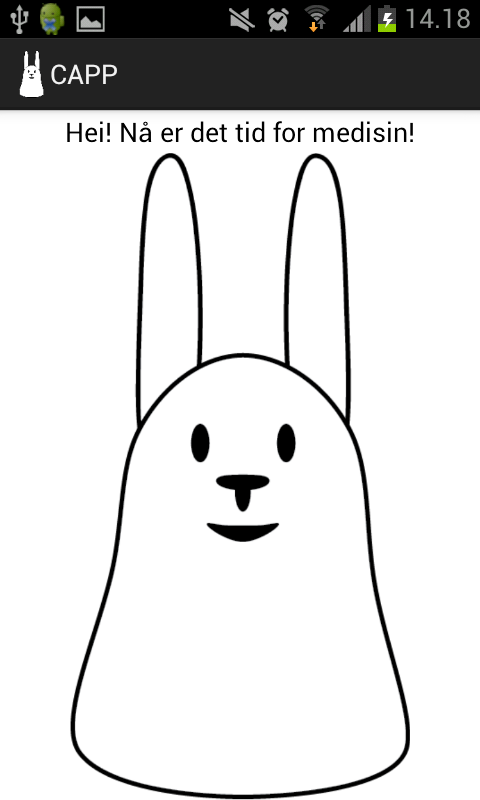
\includegraphics[width=0.20\paperwidth]{Pictures/app-screenshots/capp_start_treatment.png}
		\caption{Starting a treatment}
		\label{fig:capp_start_treatment}
	\end{minipage}
	\begin{minipage}[b]{0.3\linewidth}
		\centering
			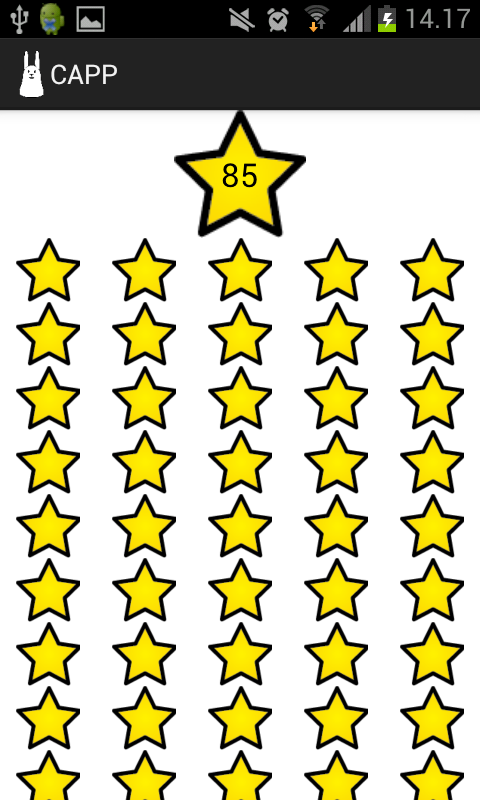
\includegraphics[width=0.20\paperwidth]{Pictures/app-screenshots/capp_stars.png}
		\caption{Inside the treasure chest}
		\label{fig:capp_stars}
	\end{minipage}
	\begin{minipage}[b]{0.3\linewidth}	
		\centering
			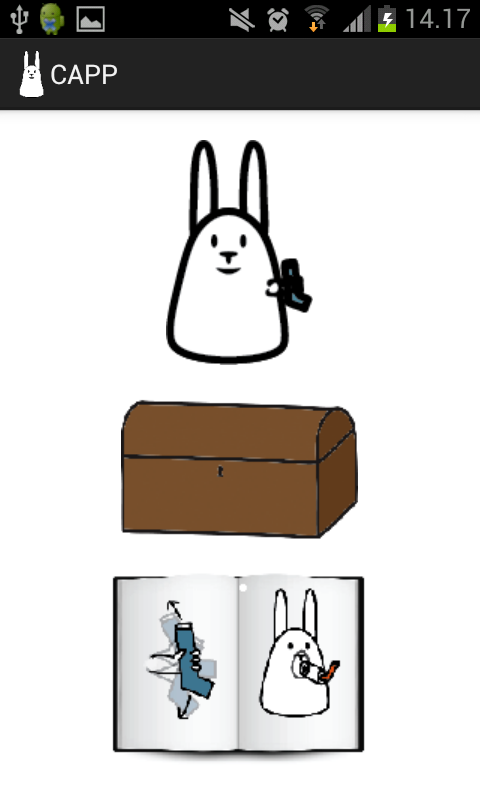
\includegraphics[width=0.20\paperwidth]{Pictures/app-screenshots/capp_main_menu.png}
		\caption{CAPP main menu}
		\label{fig:capp-main-menu}
	\end{minipage} 
\end{figure}

%INSTRUKSJONER
\begin{figure}
	\begin{minipage}[b]{0.3\linewidth}
		\centering
		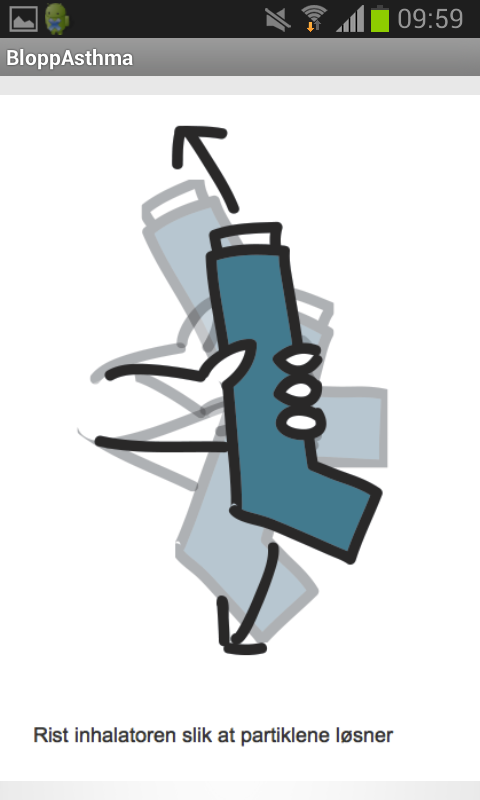
\includegraphics[width=0.20\paperwidth]{Pictures/app-screenshots/instructions-1.png}
		\caption{Instructions 1}
		\label{fig:instructions-1}
	\end{minipage}
	\begin{minipage}[b]{0.3\linewidth}
		\centering
		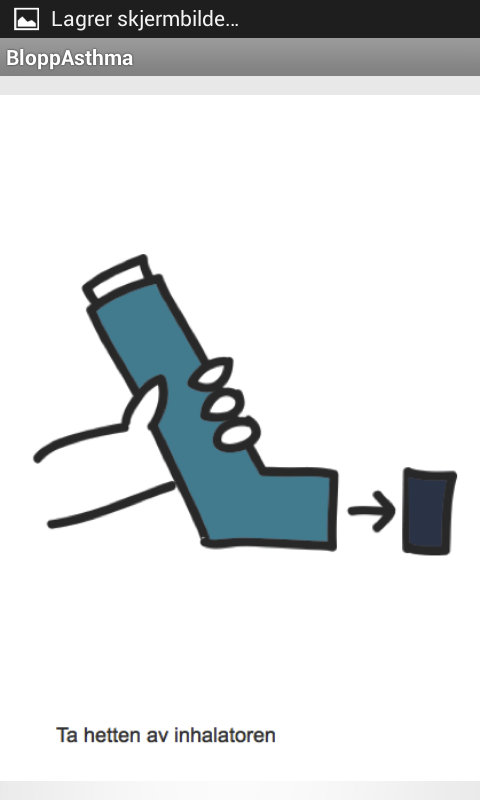
\includegraphics[width=0.20\paperwidth]{Pictures/app-screenshots/instructions-2.png}
		\caption{Instructions 2}
		\label{fig:instructions-2}
	\end{minipage}
	\begin{minipage}[b]{0.3\linewidth}
		\centering
		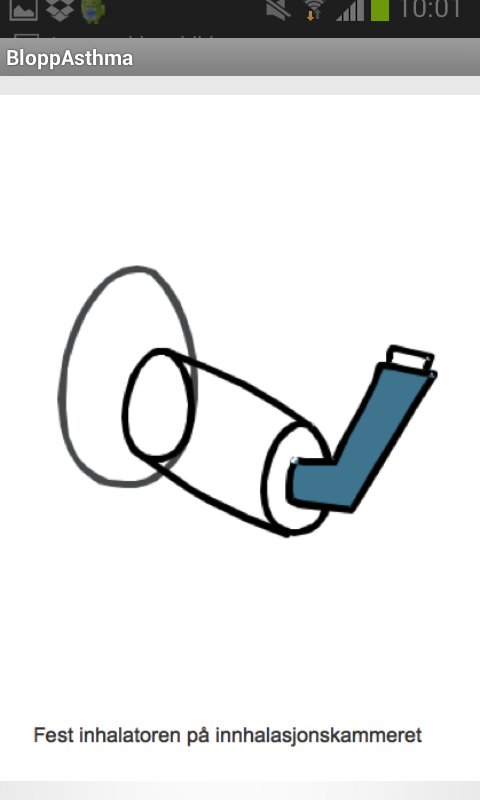
\includegraphics[width=0.20\paperwidth]{Pictures/app-screenshots/instructions-3.png}
		\caption{Instructions 3}
		\label{fig:instructions-3}
	\end{minipage}
	
	\begin{minipage}[b]{0.3\linewidth}
		\centering
		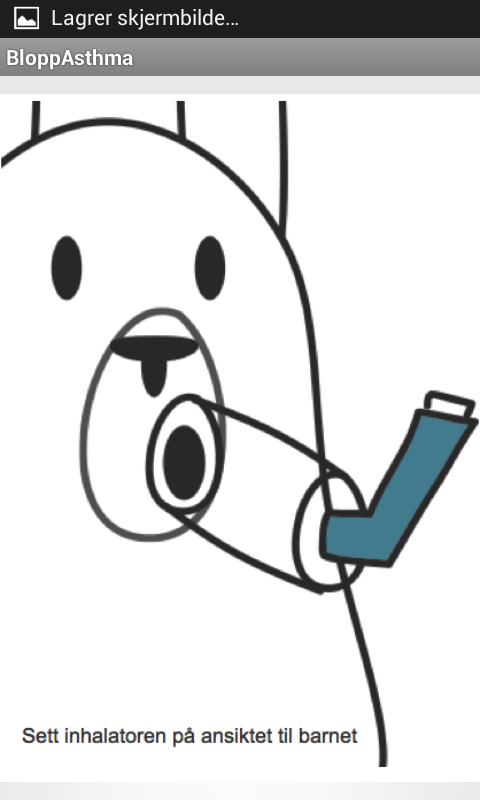
\includegraphics[width=0.20\paperwidth]{Pictures/app-screenshots/instructions-4.png}
		\caption{Instructions 4}
		\label{fig:instructions-4}
	\end{minipage}
	\begin{minipage}[b]{0.3\linewidth}
		\centering
		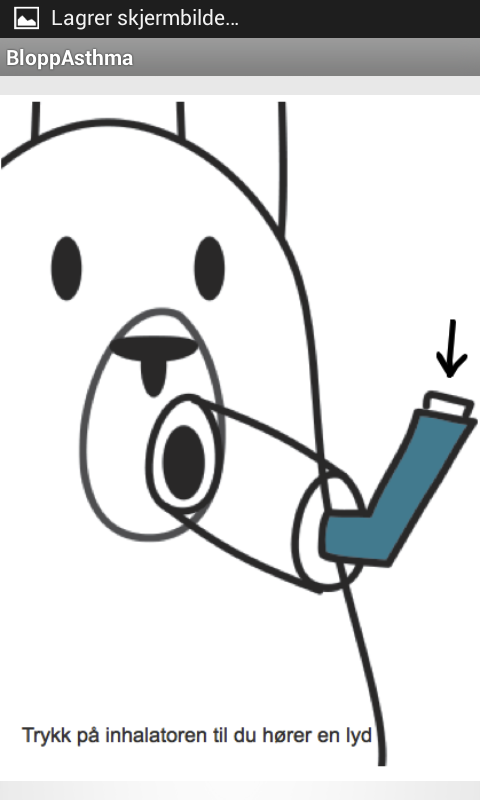
\includegraphics[width=0.20\paperwidth]{Pictures/app-screenshots/instructions-5.png}
		\caption{Instructions 5}
		\label{fig:instructions-5}
	\end{minipage}
	\begin{minipage}[b]{0.3\linewidth}
		\centering
		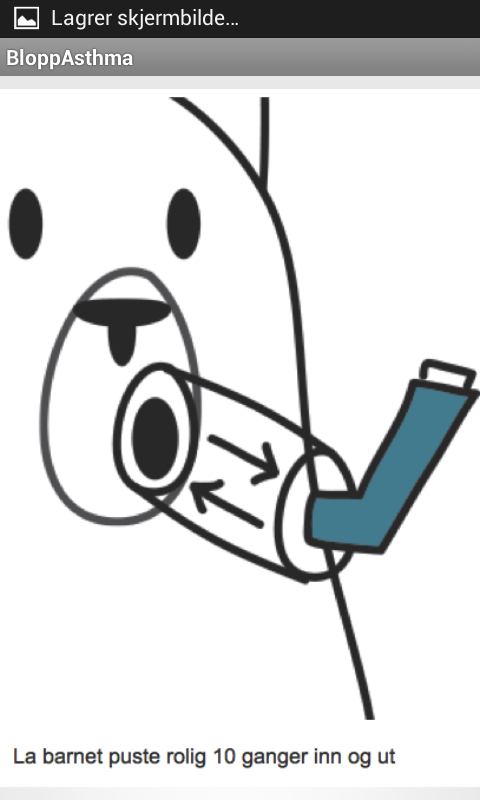
\includegraphics[width=0.20\paperwidth]{Pictures/app-screenshots/instructions-6.png}
		\caption{Instructions 6}
		\label{fig:instructions-6}
	\end{minipage}
	
	\begin{minipage}[b]{0.3\linewidth}
		\centering
		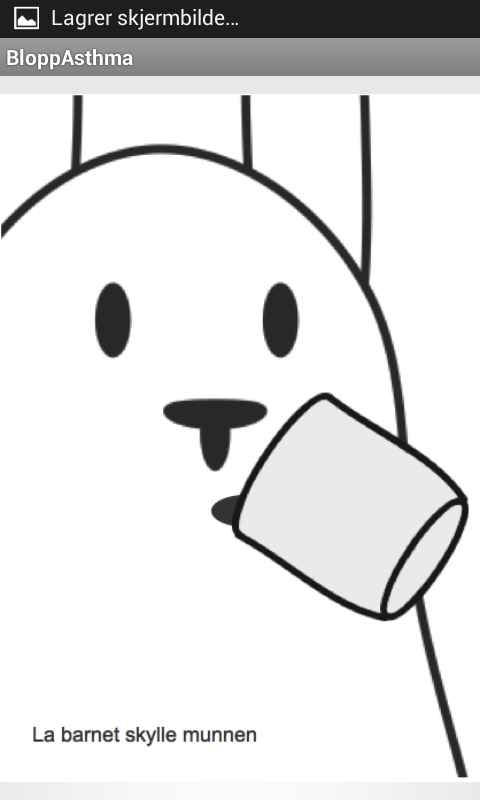
\includegraphics[width=0.20\paperwidth]{Pictures/app-screenshots/instructions-7.png}
		\caption{Instructions 7}
		\label{fig:instructions-7}
	\end{minipage}
\end{figure}


\subsection{KAPP}
\label{sec:description-kapp}
KAPP is the TUI-application targeted towards children. The application runs on a Karotz\cite{karotz}, which is a small robot bunny (see Figure \ref{fig:karotz}). The purpose of the KAPP is similar to CAPP, namely to remind children when it is time to take their asthma medicine and give instructions during treatment. In order to interact with the Karotz, children may use either a Nanoz (a small bunny with an integrated RFID) or by pressing a button on the top of the Karotz' head. It is not possible to do a by-need treatment with a Karotz as a companion. 

A basic breakdown of the CAPP and KAPP manuscript is included in Appendix \ref{chp:anuscript}. 


\begin{figure}
	\begin{minipage}[b]{0.4\linewidth}
		\centering
			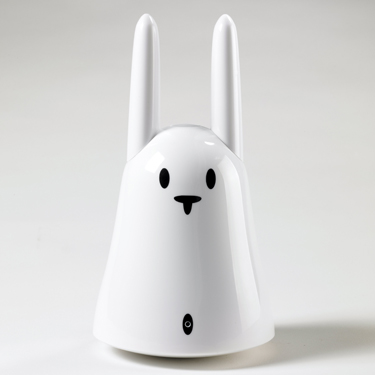
\includegraphics[width=0.20\paperwidth]{Pictures/karotz.jpg}
		\caption{Karotz}
		\label{fig:karotz}
	\end{minipage}
	\hspace{3cm}
	\begin{minipage}[b]{0.4\linewidth}
	\centering
		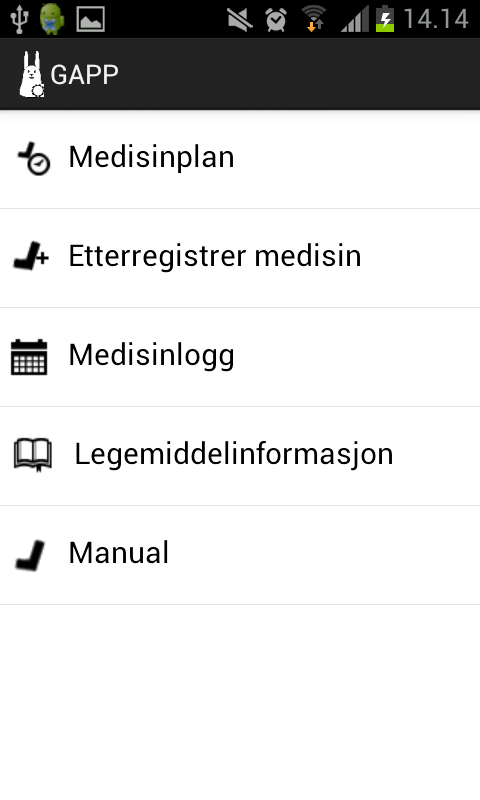
\includegraphics[width=0.20\paperwidth]{Pictures/app-screenshots/gapp_main_menu.png}
		\caption{GAPP main menu}
		\label{fig:gapp-main-menu1}
	\end{minipage}
\end{figure}


\subsection{GAPP}
\label{sec:description-gapp}
GAPP is an Android application targeted towards the parents or parents of the children. 
Some parents are having problems with remembering how often their children have taken their medication the last couple of days, when they should take them and how their children's disease has evolved over the a period of time. Thus, GAPP's main puropose is to make parents more aware of their children's disease.   


Figure \ref{fig:gapp-main-menu1} shows a screenshot of the main menu of GAPP. The main functionality is separated into 
\emph{Medical Plan}, \emph{Register Treatment}, \emph{Medicine Log}, \emph{Medical Information} and \emph{Manual}. 

\paragraph{Medical Plan}
\emph{Medical Plan} gives parents the option to set up reminders at particular times. It is divided according to the Traffic-Light system (See Appendix \ref{chp:traffic-light}). A child has three separate plans, such that an alarm that is set on the \emph{Healthy}-plan is not automatically set on the \emph{Sick}-plan.   

\paragraph{Register Treatment}
The \emph{Register Treatment}-option gives parents possibility to register a treatment that is taken in case the child for some reason did not go through the process in CAPP or KAPP. This way, children will be rewarded with stars accordingly. Figure \ref{fig:gapp-register-treatment} shows a screen shot of this process.  

\paragraph{Medical Information}
\emph{Medical Information} gives general information about different medicines, what they do, and what they are used for. The three medicines that are currently in the system is Flutide, Seretide and Ventoline. Figures \ref{fig:information-1} and \ref{fig:information-2} shows screenshots from this functionality.
%Functionality vs process  

\paragraph{Medicine Log}
\emph{Medicine Log} shows how many times a child has taken their medicine the last couple of days. Figure \ref{fig:medicine-log} shows a screen shot of this functionality. A red circle marks the current day. A child's health state is displayed by the Green/Yellow/Red bar at the top of each day. In the bottom left corner, it is possible to show how much medicine were taken at a given day.
In the bottom right corner, Aaberg et. al. intended to show the pollen distribution for a given day. However, the pollen distribution data is only available during spring and summer, and thus created an artificial pollen distribution for demonstration purposes. 

\paragraph{Manual}
The \emph{Manual} is to help ``newcomers'' to medicate children. For instance, if an aunt was watching children with asthma, she could use the application as a reference on how to do the process. At the time being, the manual shows Figures \ref{fig:instructions-1}-\ref{fig:instructions-7}. 
        
\begin{figure}
	\begin{minipage}[b]{0.3\linewidth}
		\centering
		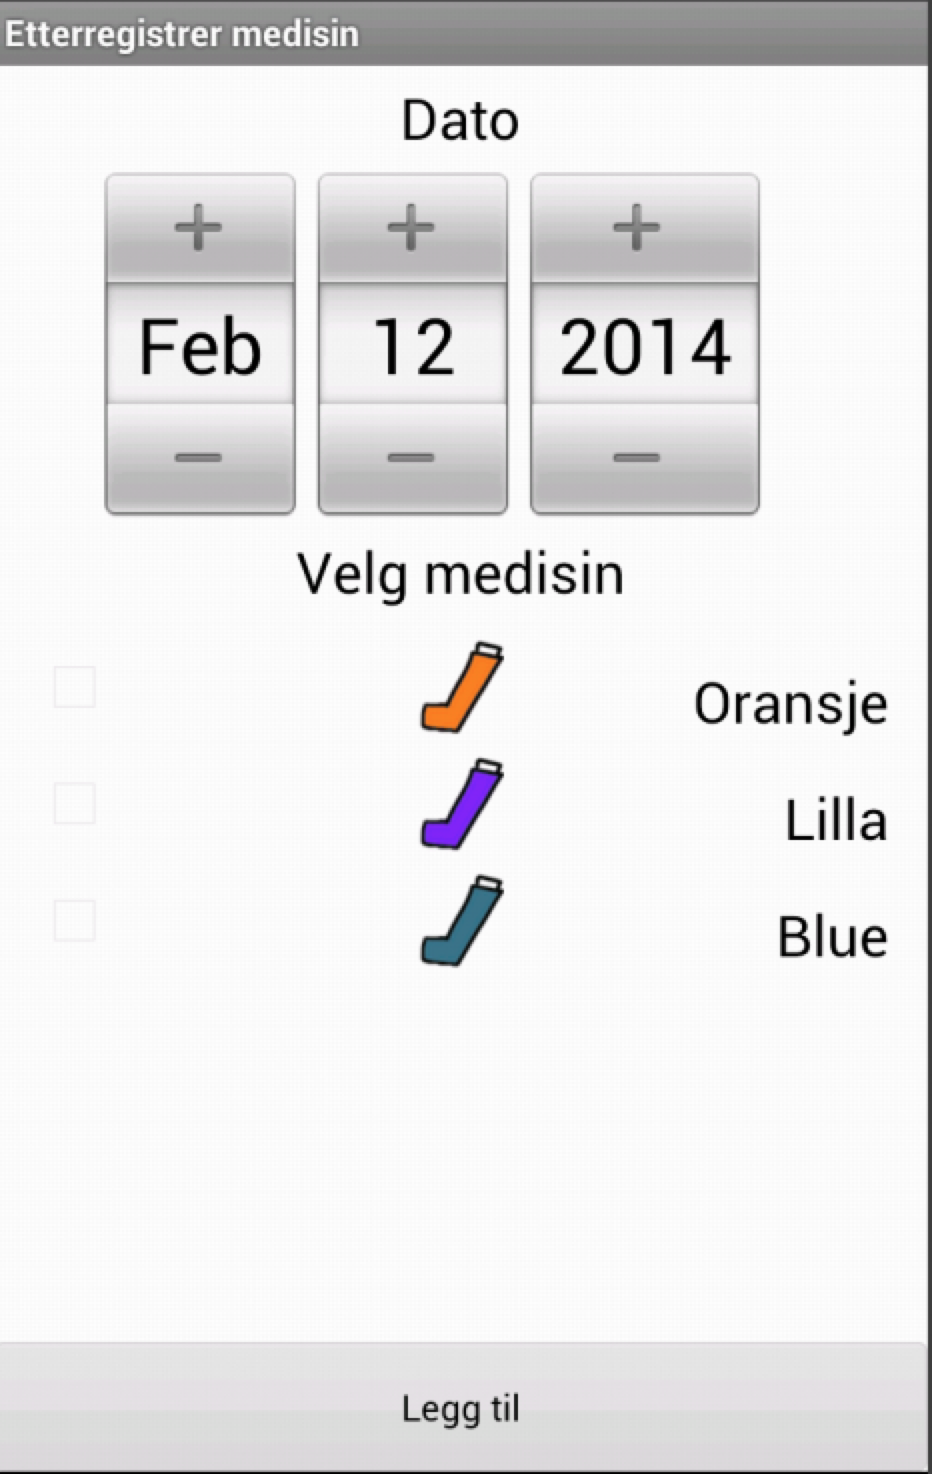
\includegraphics[width=0.20\paperwidth]{Pictures/app-screenshots/register_treatment.png}
		\caption{Register treatment}
		\label{fig:gapp-register-treatment}
	\end{minipage}
	\begin{minipage}[b]{0.3\linewidth}
		\centering
		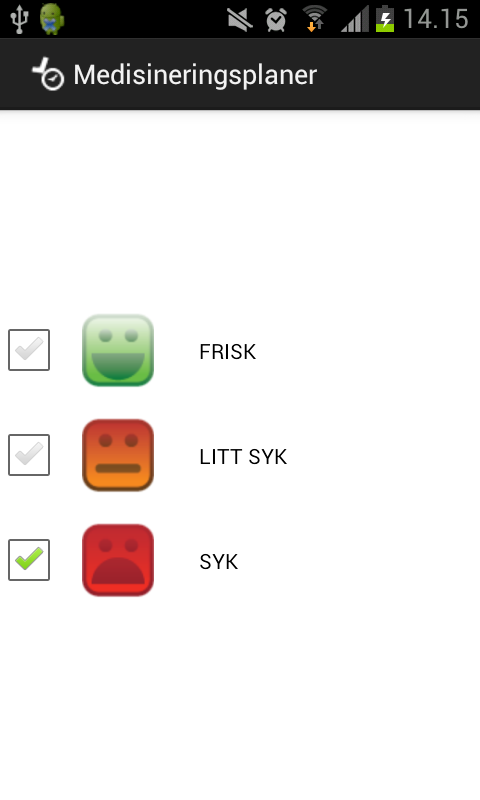
\includegraphics[width=0.20\paperwidth]{Pictures/app-screenshots/gapp_view_plans.png}
		\caption{View plans}
		\label{fig:gapp-view-plans}
	\end{minipage}
	\begin{minipage}[b]{0.3\linewidth}
		\centering
		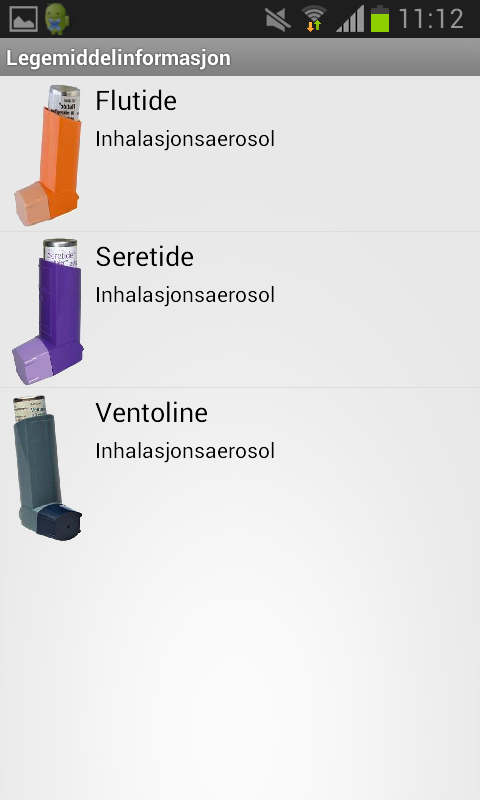
\includegraphics[width=0.20\paperwidth]{Pictures/app-screenshots/information-1.png}
		\caption{Information 1}
		\label{fig:information-1}
	\end{minipage}
	\begin{minipage}[b]{0.4\linewidth}
		\centering
		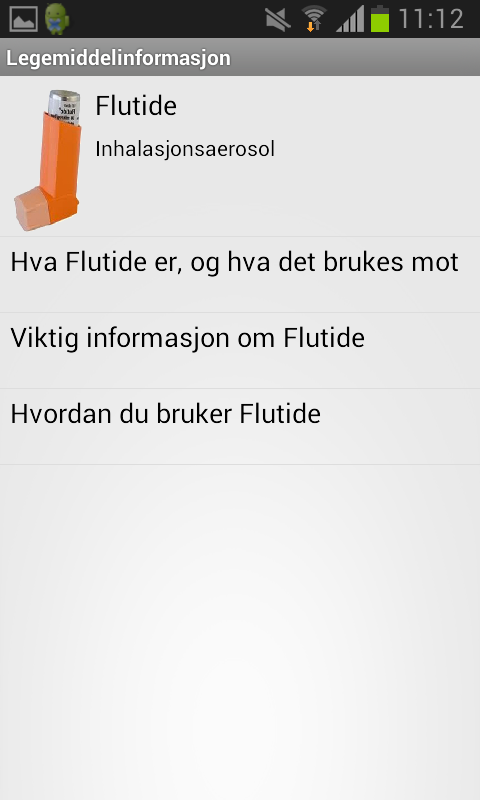
\includegraphics[width=0.20\paperwidth]{Pictures/app-screenshots/information-2.png}
		\caption{Information 2}
		\label{fig:information-2}
	\end{minipage}
	\hspace{3cm}
	\begin{minipage}[b]{0.4\linewidth}
		\centering
		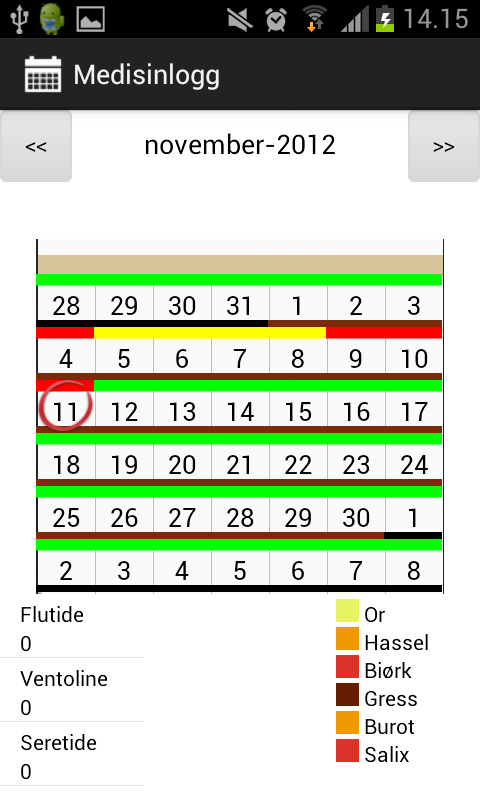
\includegraphics[width=0.20\paperwidth]{Pictures/app-screenshots/logg.png}
		\caption{Medicine log}
		\label{fig:medicine-log}
	\end{minipage}
	
\end{figure}

\subsection{Known areas for improvement}
\label{sec:improvements}
As Aaberg, Aarseth, Dale, Gisvold and Svalestuen finished their work, they commented on several areas of potential improvement for CAPP, GAPP and KAPP. This document is reprinted in its entirety in Appendix \ref{app:furtherWork} (after permission from Aaberg, Aarseth, Dale, Gisvold and Svalestuen). The main topics for improvement were
\begin{itemize}
\item{Reward System}
\item{Distraction sequence for children}
\item{Web application}
\end{itemize}


These comments are used as a basis when we decide what to improve in this project. 

\section{Existing Research}
\label{sec:existing-research}

This section will give a foundation on some of the reserach performed on using technology in combination with diseases and children. 


\subsection{Monitoring Asthma with Mobile Technology}
There exists some research on self-management of monitoring your asthma condition. A lot of this research works used SMS (Short Messaging System) technology. In 2009, Andh\o j  et. al.\cite{anhoj2004feasibility} did a feasability study to check how users would respond to a SMS-reminder study. Their methodology was to send SMS a couple of times a day, and have the users respond to their peak flow and answer yes/no questions. Users could then access a web page to see different statistics on peak flows, how they've felt the last couple of days, etc.

They concluded that SMS is a feasible solution for collecting asthma diary data, mainly because the SMS technology was a big part of the participant's everyday life. Although SMS is a great technology to be used for this purpose, few children in our target group are able to use this technology, for obvious reasons. According to \emph{Senter for IKT i utdanningen} (Center for ICT in education), about 40\% of Norwegian children below the age of 3 years old have used a tablet, and 6 out of 10 children below the age of 6 have used a touch screen device \cite{nrkchilduse}. Thus the technological background should be somewhat familiar for our target group.  


\subsection{Children and Mobile Devices}
In 2013, \url{www.babies.co.uk} posted results on a poll they had posted on how many toddlers are using smartphones or tablets each day\cite{babiesusageoftablets}. Over 1000 participants responded,  and according to the survey, 14\% of the responders allowed children to use smartphones or tablets more than 4 hours a day. Considering the normal awake time of a child between 9 and 12 months old is approximately 10 hours, they spend a considerable amount of their day on the smartphone.         


\subsection{Children and Gestures}

Abdul Aziz et. al. \cite{aziz2013children} performed a study on which gestures children are able to comprehend when playing with an iPad. She tested 33 children's abililty to do gestures on a variety of applications suited for children. The children were in the range of 2-12 years old, 3 children per age. The study showed the following restrictions:

\begin{itemize}
  \item 2 year old children have difficulties with pinching, and are unable to drag and drop, spread and rotation of the device, and are not able to focus on the application. 
  \item 3 year old children have difficulties to drag and drop until they are told to do so, in addition to having problems with pinch and spread. 
  \item 4 year old children have difficulties to drag and drop. 
\end{itemize}
Children at age 5 and above are able to do all the normal gestures at a tablet. As CAPP is currently only available for mobile devices, this is reason for some discussion. The main part to notice is pinching and drag and drop. An iPad is fairly large relative to the size of these children's hands. There is reason to believe that gestures may be more difficult on smaller screens, however, we were unable to find research supporting this claim. In order to make AsthmAPP as child friendly as possible, it only uses ``swiping'' gestures and button presses for navigation.

\subsection{Assessment of Existing Applications}
In 2012, Huckvale et. al. \cite{huckvale2012apps} conducted an assesment on the existing applications on both Google Play\fnurl{Google Play}{http://play.google.com} and App Store\fnurl{Apple App Store}{http://www.apple.com/itunes/features}. They assessed 103 different apps with english as the native language. Out of these applications, 


\emph{``No apps for people with asthma combined reliable, comprehensive information about the condition with supportive tools for self­management''} \cite{huckvale2012apps}. 


They concluded that doctors should be careful when recommending apps for patients with the purpose of self management of asthma.

\section{State of the Art}
\label{sec:stateoftheart}
Mobile computing is evolving at a rapid pace, and finding new ways to use it in health care is a rising challenge for research. This section covers the state of the technological development of some of the areas in which mobile technology is being used with a combination of either gamification or tangible interfaces.   


\subsection{Get Up and Move (GUM)}
\label{sec:gum}
Penados et. al.\cite{penadosget} created GUM; an interactive toy to measure and stimulate physical activity. GUM is a small creature that needs to be taken care of by a child. The child's objective is to make his/her GUM healthier and happier by moving with it, feeding it and playing with it. GUM is healthy and happy when it has been through a minimal amount of daily physical activity, and since GUM can not move by itself, the child needs to do it. As GUM grows healthier, lighted stars will appear in its ears, until it reaches a maximum healthy state. To increase the number of stars, the child needs to progressively increase and later maintain the GUM's physical activity level. Penados et. al. argues that GUM had a positive effect on reducing sedentary behaviour and motivate physical activity with young children.


\subsection{Sisom}
\label{sec:sisom}
Sisom\fnurl{Sisom: Si det som det er}{http://www.communicaretools.org/sisom/} is a software created to increase the communication level between physicians and children. It is an interactive game, where the user follows an avatar through different ``worlds'' of health care subjects. For instance, the avatar takes a boat to a hospital. The user can look around in the hospital and express how he/she feels when giving a blood sample. The results showed that when a child played the game before a consultation with his/her physician, the child was better prepared, the communcication had a better quality, and the child participated more during the consultation\cite{sisom-research}.


\subsection{Meassuring Blood Pressure}
\label{sec:bloodpressure}
iHealth\fnurl{iHealth}{http://www.ihealthlabs.com/wireless-blood-pressure-monitor-feature\_32.htm}, Withings\fnurl{Withings}{http://www.withings.com/en/bloodpressuremonitor/features} and other companies has created blood pressure monitors which are synchronized with mobile applications. By using a wrist monitor; heartbeat, blood pressure level and pulse wave is meassured and stored in the application. The application visually presents graphs of the user's historic blood pressure levels and tracks progress. The application also allows for sharing meassurements with friends, family and doctors. By sharing detailed information with a doctor, a more accurate treatment plan may be laid out.


\subsection{Controlling Your Diabetes}
\label{sec:controldiabetes}
Cellnovo\fnurl{Cellnovo}{http://www.cellnovo.com/} has created a system that helps users to control their diabetes. It consists of a handheld device for meassuring blood sugar levels, a pump that controls the flow of insulin and a web interface that allows one to access the information. The interface helps users to check for trends and patterns in their blood sugar level, which again motivates users to continue applying the correct treatment. It also allows users to send information to physicians, which helps them make decisions regarding patient care.
      

\subsection{Quit Smoking}
\label{sec:quitsmoking}
There are lots of mobile applications that help people to quit smoking. For instance, \emph{The Norwegian Heart and Lung Patient Organization} has developed an app called ``'R\o ykeslutt''\fnurl{R\o ykeslutt}{https://play.google.com/store/apps/details?id=no.lhl.roykeslutt}. The application shows what the body is going through after a specific amount of days after the user has stopped smoking, which according to the reviews of the application, is a huge motivational factor. Additionally, they show how much money a user has saved at any given time, which can be seen as ``gamifying'' the element of money in order to motivate users.  


\subsection{TUIs and Multimodal Interfaces for Safety-Critical Applications}
Cohen \etal{} proposed the use of TUIs and Multimodal Interfaces(MMUI) for safety-critical applications \cite{cohen2004tangible}. They present an example with making strategic military planning of a battlefield. By combining special pens with cameras, CPUs and communication units, the lines drawn on a physical map would easily translate to a digital one. These tools made it easier to collaborate on making strategies and sharing them between officers. Cohen \etal{} argues that the combination of TUIs and MMUIs may make a suitable improvement for traditionally paper-heavy work.

\subsection{Exercise Games}
\label{sec:exercisegames}
In the last few years the exercise equipment industry has embraced gamification through their products. The use of experience points, badges, milestone goals and progress bars are commonly used to market products. Following are two, of many possible, examples of how the industry has made use of gamification. 

In 2012 Nike launched their Nike+ Fuelband\fnurl{Nike+ Fuelband}{https://secure-nikeplus.nike.com/plus/what\_is\_fuel/}, a wearable device for tracking the user's activity level. The Fuelband is worn as a bracelet, and has small LED lights indicating how active the user has been during the day. By being active the user collects NikeFuel\texttrademark, lighting more LED lights on the bracelet. The user may set goals for how active he/she should be in order to collect enough NikeFuel for the day. 

Nintendo Wii has gamified the way people exercise at home with Wii Fit and later Wii Fit Plus\fnurl{Wii Fit}{http://wiifit.com}. It gives a user the ability to choose his/her own training programme, including Yoga, Strength and Aerobics. The user can easily track his/her progress over several months. Additionally, it contributes to keeping children healthy, by having games that depend on the child's movement. For instance, if a child flaps his/her arms up and down, a bird on the screen is able to fly.
 
 % Background Theory 

\chapter{Gamification}
\label{chp:gamification}

This chapter will give a description of the term ``gamification'', describe some of the uses of gamification and how we plan to use gamification in our solution.

\section{What is Gamification?}
\label{sec:whatisgamification}
``Gamification'' as a term was first mentioned by Currier in 2008\cite{gamificationcurrier}, but did not become a wide-spread term until 2010. 

Huotari and Hamari\cite{huotari2012defining} define gamification as:

\textit{``Gamification is a process of enhancing a service with affordances for gameful experiences in order to support user's overall value creation.''}

There are many different ways of describing gamification. Deterding, Dixon, Khaled and Nacke\cite{Deterding:2011:GDE:2181037.2181040} define Gamification as:

\textit{``Gamification is the use of game design elements in non-game
contexts.''}

Deterding, Dixon, Khaled and Nacke's definition is often commonly referred to, because of its simplicity and understandability for people who have little or no connection to traditional video games or game consoles.

Today gamification is a much used term both in programming and in the spoken language. Smartphone applications and manufacturers have helped make the term gamification a widespread notion. Examples of this is the application Foursquare, which is built around gamifying ``checking in'' at restaurants, historical sites and similar places\fnurl{Foursquare}{www.foursquare.com}. Apple developed a Game Center for iOS in 2010, giving every iPhone/iPod and iPad user a hub for challenges, awards and other gamelike activities\fnurl{Apple Game Center}{http://support.apple.com/kb/HT4314}, which made every iOS user a potential target for gamification. Lately there have been many games built singularily around gamification, such as Cookie Clicker\fnurl{Cookieclicker}{http://orteil.dashnet.org/cookieclicker/} or Farmville\fnurl{Farmville}{www.farmville.com}. Even game consoles like Playstation 3 and Xbox contain gamification support per default, with their achievement/trophy systems\fnurl{Xbox}{http://xbox.com}\fnurl{Playstation}{http://playstation.com}. While there are many users of such games, they are often criticised for using gamification to lure players into playing. 


\section{What are Serious Games?}
\label{sec:seriousgames}

The term ``serious game'' became a concept with the emergence of the Serious Game Initiative in 2002\cite{seriousgamesinitative}. Their website defines serious games as: 

\textit{``The Serious Games Initiative is focused on uses for games in exploring management and leadership challenges facing the public sector. Part of its overall charter is to help forge productive links between the electronic game industry and projects involving the use of games in education, training, health, and public policy.''} 

This definition has been criticised for being too narrow, and for not including any reason as to why businesses should care. An anonymous author\footnote{The essay is only signed with the name 'Danc'. Still, we regard this essay interesting and relevant, and it has been mentioned in several scientific publications.} posted an essay on \url{www.lostgarden.com} criticizing the definition and suggesting the following definition:

\textit{``Serious Games: The application of gaming technology, process, and design to the solution of problems faced by businesses and other organizations. Serious games promote the transfer and cross fertilization of game development knowledge and techniques in traditionally non-game markets such as training, product design, sales, marketing, etc.''}


Since it's debut in 2002, serious games have later grown to become a multi-billion industry.
Pilots are being trained in simulators, lecturers make lecture quizzes for students\cite{wang2007lecture}, Swedish firefighters have used serious games for training\cite{lebram2009design} and persons suffering from diabetes can use serious games for learning about the illness. These are just a few of the many ways of using serious games. 

Foldit is a very interesting example of how a serious game may lead to solving bigger problems than the game itself\cite{cooper2010predicting}. Foldit is a massive multiplayer online game (MMO). The objective for the player is to fold protein by following a set of rules. The system records how players fold protein and learns patterns for interaction. Humans have much higher skills at interacting with 3D objects than computers, and the system learns patterns and techniques from the players. By playing Foldit, researchers were able to solve the crystal structure of the M-PMV retroviral protease\fnurl{Mason Pfizer Monkey Virus}{http://microbewiki.kenyon.edu/index.php/Mason\_pfizer\_monkey\_virus}\cite{khatib2011crystal}.

Serious games and gamification have many similarities; whereas serious games are mainly targeted towards making education or learning more fun, gamification is used in a number of different ways. 


\section{Discussion about Gamification}
\label{sec:gamificationdiscussion}

Gamification is a much discussed theme, and no agreement seems to have been reached as to whether gamification is useful or not. 
Antin and Churchill argues that gamification may be used for goal setting or instruction\cite{antin2011badges}. Goal setting challenges the users to meet the mark that is set for them, and is known to be an effective motivator\cite{ling2005using}. 

Bogost goes as far as naming gamification as ``marketing bullshit'', used as a way of moneytizing bad business\cite{gamificationbullshit}\footnote{While this is not a scientific publication, we found it interesting and relevant to the discussion}.

McGonigal's studies on how rewards are perceived over time show that: 

\textit{``After three hours of consecutive online play, gamers receive 50 percent fewer rewards (and half the fiero\footnote{Fiero is an italian term for personal triumph\cite{ekman2007emotions}}) for accomplishing the same amount of work.''}\cite{jane2011reality}

Steinung argues that gamification is not powerful enough to make a task interesting\cite{steinung2012interessante}. Simply adding points, badges, a leveling system or similiar, will not make a task interesting on its own. Since gamification is based on behavioural pshychology, poor design may be perceived as interesting, for a shorter period of time\cite{steinung2012interessante}. Zichermann makes a similar statement, saying gamification needs to take ethical precautions\cite{zichermann2011gamification}.

While McGonigal's research focuses on how rewards are percieved when playing over a longer consecutive time, our intent was to make the user spend only small amounts of time using the application. AsthmAPP is a tool, not a pastime.

In order to achieve a meaningful use of gamification Nicholson\cite{nicholson2012user} suggests using a user-centered design approach\cite{usercentereddesign} when developing systems with elements of gamification. Since AsthmaBuddy is a computer supported learning system\cite{stahl2006computer} it was important for us to maintain our focus on the learning and awareness created by our system, making gamification a tool and not the key feature.

\section{Game Elements}
\label{sec:gameelements}

This section will take a brief look into the different classifications of players that exists, and will introduce the reader to the mechanisms commonly used to gamify users' experiences. 

\subsection{Bartle's Four Player Types}
\label{sec:bartlesplayertypes}
People have different preferences when it comes to playing a game. Richard Bartle proposes a classication of four different player types\cite{bartle-gamers}. These types are \emph{Achievers},  \emph{Explorers},  \emph{Socialisers} and \emph{Killers}. We'll take a brief look on each of these in this section. 

\subsubsection{Achievers}
\textit{``Achievers regard points-gathering and rising in levels as their main goal, and all is ultimately subserviant to this''}\cite{bartle-gamers}. 

Most young children will fall under this category. Achievers mostly play games just for the fun of it, and do not necessarily need other incentives to the game than being able to finish the challenge imposed by the game. Most children like to see progress in terms of points, clearing a level or a similar sense of progression. 

\subsubsection{Explorers}
\textit{``Explorers delight in having the game expose its internal machinations to them''}\cite{bartle-gamers}.

Explorers are thus the players who easily enjoy a game more than once, and potentially want to find every secret embedded in the game. Children will in some cases fall under this category, but with our target group, it is hard to separate between achievers and explorers. 
[Children play the game for the fun of playing, not necessarily to find discover secrets][Find something that supports this claim] 

\subsubsection{Socialisers}
\textit{``Socialicers are interested in people, and what they have to say. The game is merely a backdrop, a common ground where things happen to players''}\cite{bartle-gamers}. 

This implies that socialisers play games in order to connect with new people or hang out with their friends. The youngest children in our target group will probably noy fall under this category, as they will not comprehend that there is someone ``on the other side of the screen''.    

\subsubsection{Killers}
\label{sec:killers}
\textit{``Killers get their kicks from imposing themselves on others''}\cite{bartle-gamers}.

``Killers'' thrive upon destroying other people's game experience. Hopefully, no children fall into this category, at least not in our target group. [Something about social skills not developed yet?] 

\subsection{Game Mechanisms Used to Achieve Gamification} 
\label{sec:gamemechanismsusedtoachievegamification}
There are some game mechanisms that are widely used for gamifying every day tasks. This section will explain some of them. We will use a stick figure to examplify each game mechanism. 

\subsubsection{Avatar Systems}
\label{sec:avatarsystems}
Avatars are commonly used in children's games. It gives a player a virtual character, which can be upgraded with different clothing and equipment when players reach certain points in the game. Such equipment can usually be bought for either points awarded or through \emph{In-app purchases}. Players can then show their avatar to other users, compare, and have fun with them. This approach may be seen as giving the avatar a piece of the player's personality. For instance, some players would want their avatar to look as ridiculous as possible, while others would prefer that it looked as cool as possible. Showing off ``expensive'' gear may also give the player a feeling of accomplishment (\emph{``I'm so good at this game that I could afford this golden armour. Have you managed to get it yet?''}). 

\textbf{Example:} The stick figure will be a player's avatar, which can be modified to have different pieces of clothing or equipment.  

\subsubsection{Achievements and Badges}
\label{sec:achievementsandbadges}
Achievements and badges are systems well incorporated into Microsoft's Xbox\fnurl{Xbox}{www.xbox.com} and Sony's Playstation\fnurl{Playstation}{www.playstation.com}. Such achievements and badges are typically given if the player reaches a certain point or level in the game. For instance, on Foursquare, the players gets a badge called ``Adventurer'' if he/she checks in at 10 different venues. 

\textbf{Example:} If we combine this mechanism with avatar systems, we can give out a badge when the stick figure has obtained a complete sets of clothes or a specific set (eg. has purchased all the green clothing).   

\subsubsection{Real-world Rewards}
\label{sec:realworldrewards}
Used together with leaderboards, real-world awards may be given to some of the best players of the game. For instance, they could be rewarded with exclusive tickets to concerts. These real-world awards are often given during marketing campaigns, for instance ``Invite your friends to use this system, and recieve one ticket in the lottery to win a brand new computer''.  

\textbf{Example:} Players may have a real-life stick figure, and the stick figure is rewarded with equipment sent to the player by mail. These rewards could be, for example, different clothing or equipment the player could apply to the figure. 

\subsubsection{Social networking}
\label{sec:socialnetworking}
During the last few years, Facebook feeds has a tendency to be flooded by updates from third-party applications, like Runkeeper\fnurl{Runkeeper}{http://runkeeper.com/}, who updates everyone on your friend list that you have been working out. The idea here is to have a common platform, where users may brag about their accomplishments.      

\textbf{Example:} Social networking may be used to upload images of a player's stick figure, and show it to his/her friends. 

\subsubsection{Mirroring User Behaviour}
\label{sec:mirroringuserbehaviour}
This is most commonly used for children, where an animation or a character shows how to go forward with a procedure. For instance, there are a lot of apps on App Store mirroring the process of brushing a child's teeth. A child may use this app as a reference that indicates how long he/she should brush on the same side.   

\textbf{Example:} The stick figure mirrors the player's intended behavior. 

\subsubsection{Experience Points}
\label{sec:experiencepoints}
Experience points is an indicator of how much experience the player has gaines within a game or setting. These points may be awarded from completing tasks, exploring areas and features or other similar activities. Experience points are usually combined with a leveling system, where the player ``climbs a ladder'' using these experience points, for example by unlocking new levels, new rewards or new features. A player with many experience points is considered an experienced user, and is percieved as higher ranking than a player with less experience points. Experience points are also often combined with leaderboards. 

\textbf{Example:} One experience point may be represented as a stick figure, and the goal is to gather as many stick figures as possible. Another example is that leveling up, based on experience points, may be represented by the size or attributes of your stick figure.

\subsubsection{Leaderboards}
\label{sec:leaderboards}
A leaderboard is a list of the players ordered by their collected points, completed activites or any other predefined system. Each user has a score defined by rules set before a competition started. The score is compared and the players are ranked based on the scores. Leaderboards may be fully dynamic, changing when a player has scored points, or state based, where the new order is determined after a certain period of time.

\textbf{Example:} If the stick figure gathers enough experience points, it may find itself on a regional leaderboard, ranking players in your area (neighbourhood, town, country, etc). 

\subsubsection{Progress Bar}
\label{sec:progressbar}
A progress bar is used to indicate how far a user has come towards a given goal. When the player completes a task or an activity, the progress bar is filled to indicate the progress of getting closer to a goal. How much the progress bar is moved is often determined by the severity of a task or by using points. The progress bar may often be combined with experience points, where the experience points collected determines the movement of the progress bar. 

\textbf{Example:} The stick figure is placed on a road. The figure's position on that road, mirrors the progress a player has made. When completing a task, the figure will be moved closer to its goal.  


\subsubsection{Contests}
\label{sec:contests}
Gamification can be done through having contests either with players in a duel-like head-to-head contest or a free-for-all contest with no limit on the capacity of players. A duel-like contest may be a knockout style of competition where players compete to get the highest amount of points within a given time period or a similar type of a goal. A player may make progress in the tournament without being the player with the highest score, but being better than his/hers opponent. In a free-for-all contest, the winner is whoever fulfills a specific goal to the best degree. The goal which players try to achieve is set be a specific set of rules determined before the start of the contest.

\textbf{Example:} A player's stick figure may enter a voting contest, where votes are given to the best looking one.

\subsection{Combining Game Mechanisms in AsthmAPP}
\label{sec:combininggamemechanismsinasthmapp}
\begin{table}[H]
\begin{tabular}{| p{2.5cm} | p{2.1cm} | p{9.5cm} | }
	\hline
	\textbf{Mechanism} & \textbf{Included in AsthmAPP} & \textbf{Rationale} \\
	\hline
	Avatar systems & No & We did not have time to implement this during our thesis, but we do believe this could be a good feature if it was implemented in a right manner.    
	 \\
	\hline
	Achievements and badges & No & We believe our target group would not enjoy this feature as much as older children, those of 12 - 16 years of age.  \\
	\hline 
	Real-World awards & Yes & Children enjoy the feeling of being rewarded with something real.
	 \\
	\hline
	Mirroring user behavior & Yes & Demonstration has a positive effect on children.
	\\
	\hline
	Leaderboards & No & There are no way to implement this in a realistic and legal way. Children would have to share their data, which consists of points based on medicine doses. Parents could be blamed if their child were on the bottom of the list. It would also be negative for small children's motivation if they have been really good at taking their medicine, and perform poorly on a leaderboard. 
	\\
	\hline
	Social networking & No & Much of the same reasons as why we did not choose leaderboards. We also believe that children in our target group would not understand this aspect.  
	\\
	\hline
	Progress bar & No & In an ideal world, we could have shown how close the child was to becoming fully treated for asthma. However, identifying how close a patient is to becoming healthy, is virtually impossible. Another usage may be to match the child's progress for each week against his/her medicine plan. This would however, imply that by-need treatments would not be included, which may seem unfair for the child. Additionally, their progress would be deleted every week, which would not have much motivational effect.  
	\\
	\hline
	Experience points & Yes & The stars will work as experience points, which may used to cash in rewards from the parents. 
	\\
	\hline
	Contests & No & Using medical history to participate in contests would be a violation of Norwegian privacy laws. It may also be used to pinpoint ``bad'' parents.      
	\\
	\hline
\end{tabular}
\caption{Assessment of different game mechanisms}
\label{tab:game-mech-in-astmapp}
\end{table}

[This table should probably go somewhere else]


\section{Summary}
\label{sec:gamificationinapp}

Stapleton argues that:

\textit{``A variety of [serious game] applications can be thought of here [in Health Care] such as games as a form of motivation and reward for patients undergoing some form of treatment. Games could also be to distract patients during certain procedures such as dental work, for example."}\cite{stapleton2004serious}


Stapleton's argument is one the reasons for why we believe in the use of tangible user interfaces and applications as a method for treating children with asthma. Children are easily distracted, and we believe that making the treatment into a serious game will distract the children enough to forget what they are doing and instead look on the treatment process as a fun game.


In AsthmAPP we aimed to use gamification as a distraction and rewarding element for the children. Instead of putting a lot of predefined badges, rewards, experience points or other rewarding elements, we let the users choose their own rewards, which implies that users may decide what works best for them. This stands to reason with the arguments of Nicholson regarding how to design gamification\cite{nicholson2012user}.

As McGonigal's studies show, the effect of gamification tends to wither down after a longer period of time\cite{jane2011reality}. We aimed to solve this problem by letting the user, together with his/her parents, choose his/her own rewards. While putting the responsibility for the reward system in the hands of the user will lead to more work for the user, we believe that the positive effect of the reward system will make it worthwhile. 
 

The children are rewarded with stars based on their health state. The rationale behind this is that the children may have to take more medicine when they have a cold or there is a lot of pollen in the air. The parents have access to a administrator menu where they may set new rewards for the children. The children will then be able to order the rewards when they have earned a sufficient number of stars. This way the parents and the children create their own gamification environment. Examples of possible rewards could be to give the child an extra 10 NOK in weekly allowance, taking him/her to soccer matches or even to the local amusement park. It is an option where the only boundary is the imagination and how much cost and effort parents wish to invest in it.    


The rewards will appear on a ``milestone'' basis. We do not want children to feel they lose something if they spend stars on a reward, which some may feel as if stars were taken away from them. We do not want to force parents into giving away rewards they can not afford or do not wish to give. The use of the reward system is optional and decided by the user, making the user in control of how they wish to gamify the experience. 
We do not wish to have the children spending too much time using the application, since using a tablet or phone at such a young age is considered unhealthy. This had some implications on the complexity of our gamification system. 



\chapter{Tangible User Interfaces}
\label{chp:tangibleinterfaces}

This chapter will introduce the reader to \emph{tangible user interfaces}, and elaborate on some existing research that has been done on the concept. In addition the chapter will describe how we intend to make our tangible user interface.   

\section{About Tangible User Interfaces}
\label{sec:abouttuis}

In 1997, Ishii et. al. presented an article called ``Tangible Bits: Towards Seamless Interfaces between People, Bits and Atoms'' \cite{ishii1997tangible}. They established the term ``Tangible User Interface'' (TUI) as a way to move beyond the dominant model of Graphical User Interfaces (GUI). 
While GUIs show information (bits) in the form of pixels mapped to a display, Ishii meant that TUIs would represent the bits in form of physical objects. The objective of TUI was explained as to \emph{augment the real physical world by coupling digital information to everyday physical objects and environments}\cite{ishii1997tangible}. 

``Urp''\cite{underkoffler1999urp} is an example of an first-generation TUI. Urp is a workbench architects used to determine shadow patterns for models of buildings. By moving a ``clock tool'' the lighting on the workbench would move according to what time of day was choosen. Instead of interacting with the lights directly, the TUI factor of the workbench was the clock tool.
What made this a first-generation TUI are the fairly simple and state-determined operations.

``Sandscape''\cite{ishii2004bringing} is an example of a second-generation TUI. Sandscape uses clay, sand, cameras, digital software and lighting to give an overview of a Geographical Information System(GIS). The users could interact with the clay, forming dunes or dig holes and the software would calculate landscape analysis based on the interaction. Sandscape is dynamical user interface since it may change to several different non-predefined states, also named a ``continuous TUI''.

In 2008, Xie et. al. performed a study on how children reacted using different interfaces in order to solve a jigsaw puzzle\cite{xie2008tangibles}. The different interfaces were a physical interface (i.e. a standard jigsaw puzzle), a TUI and a GUI. Their main finding was that children enjoyed playing with the different interfaces equally. However, the children were more likely to start a puzzle over again if the interface were physical or tangible, which implies that a repeated task is more likely to be performed if the children are playing with a tangible or physical interface, while it becomes boring to do the same task over and over again on a graphical user interface. It is worth mentioning that the puzzles were being solved by groups of two, and considering the GUI was a computer with one mouse, the children did not get the same sharing experience as with the other interfaces. 


\section{Examples of Use}
\label{sec:tuiexamples}
Using TUIs instead of GUIs has been proven to work in several different settings. In this section, we will give an overview on some of the domains in which the concept has been proven to work. 

\paragraph{Learning}
Terrenghi \etal{} designed a cube for learning, giving children quizzes where answers had the shape of text or images\cite{terrenghi2006cube}. Children could then rotate the cube in order to get the correct answer pointing upwards, like a dice. They concluded that the TUI gave children a different set of affordances that prompted a great initial engagement\cite{terrenghi2006cube}. 

\paragraph{Information Sharing}
Hinckley et. al. created a tangible user interface for neurosurgical vizualisation\cite{hinckley1994passive}. Their tool proved helpful for neurosurgeons to provide physical familiar tools that could display information digitally. Their tool showed possibilities for creating and view cutting planes and planning neurosurgery. Their tool made it easier for them to display the surgical cutting planes to other persons with less knowledge in neurosurgery, or to other surgeons. 

Moran et. al. designed a physical wall for sharing information on people in an office\cite{moran1999design}. The system, named ``Collaborage'' showed a person locator and different types of project information. Collaborage showed how the use of traditional use of walls and sticky notes translated into a digital software in a positive manner.


\paragraph{Collaborative Learning}
Scarlatos et. al. created a system called TICLE (Tangible Interface in Collaborative Learning), which are used to help children solve a Tangram\cite{scarlatos1999ticle}.  


\paragraph{Interactive Storytelling}
Zhou et. al. designed a cube for storytelling, using a head mounted display and a ``magic story cube'' in order to let children explore the world while being told a story\cite{zhou2004magic}. Stanton et. al. created a ``magic carpet'', giving children possiblity to influence a story in the classroom\cite{stanton2001classroom}. 

 
\paragraph{Social Context}
``Marble Answering Machine'' is an invention by Durrell Bishop, dating back to 1992\cite{crampton1995hand}. The interface allows users to drop marbles into a play-back indent on the system, which plays a recorded message.   


\section{TUIs Used in Health Care}
\label{sec:effectofrobots}
In 2003, Wada et. al. conducted a study on how the introduction of robotics affected the elderly\cite{wada2004effects}. They conducted a study at a day service center in Japan, where they placed a robotic seal, named Paro, together with the elderly. It had recently been found that animals have a positive effects on blood preassure, depression and loneliness. They placed a robotic seal in the care center, and analyzed the reactions from the elderly. 

The results showed that the elderly were in a better mood after interacting with Paro over five weeks, and became worse once Paro was removed. In addition, nurses' burnout rate decreased during the experiment, which implied that they had easier days when Paro was there. The study showed that the elderly's quality of life improved after Paro was introduced.           

Farr \etal{} did a study on children with Autisitic Spectrum Condition (ACS), when playing with a TUI called Topobo\fnurl{Topobo}{http://www.topobo.com/}\cite{farr2010social}. The study compared the level of social interaction when playing with Topobo, compared to playing with LEGO. Their findings showed that ACS children were playing more cooperatively with the TUI than LEGO. Additionally, children with traditional development were able to play more cooperative, solitary and parallell when using a TUI, suggesting that 

\textit{``(\ldots) programmable digital technology may support more pathways to social interaction.''}

\section{Paradigms in Tangible Interfaces}
Ullmer states that a tangible user interface should embody the following four properties\cite{ullmer2002tangible}:

\begin{enumerate}
	\item{Physically Embodied}
	\item{Physically Representational}
	\item{Physically Manipulable}
	\item{Spatially Reconfigurable}
\end{enumerate}

Ullmer further states that these four properties describe physical artifacts as representations and controls for digital information. 

Ullmer proposes three different paradigms of tangible interfaces; \emph{Token and Constraints}, \emph{Interactive Surfaces}, and \emph{Constructive Assemblies}. These classes are partly based on varying degree of support for continuous and discrete forms of interaction\cite{ullmer2002tangible}.

\subsection{Token + Constraint Approach}
The ``Token + Constraint'' approach centers on a hierarchical relationship between tokens and constraints. Tokens may be placed within or removed from the compatible constraints. The physical shape of the tokens and constraints display whether or not the tokens are compatible or not. This approach support a combination of continuous and discrete interactions. 

\paragraph{Strenghts of token + constraint approach}

Ullmer states that interpretive constraints will help to express which of the physical tokens can take part within a given interpretive constraint, which physical configurations these physical tokens can take and the demarcation between interaction regions with different computational interpretation.

These interpretive constraints may help to simplify the human perception since humans are good at comparing shapes and forms. 
It may help human manipulation since interpretive constraints provide an increased sense of kinesthetic feedback from the manipulation of tokens. 

\subsection{Interactive Surfaces}
In this paradigm, users manipulate physical objects upon an augmented planar surface \cite{ullmer2002tangible}. These objects are then tracked, interpreted and graphically mediated through the surface. A popular usage of interactive surfaces is to create interactive workbenches, where objects are configured upon a horizontal workbench. For instance, metaDESK with the Tangible Geospace application, had a large map of a city as it's workbench \cite{ullmer1997metadesk}. Combined with magnifying glass, it allowed users to look at 3D models of particular places in a town. 



\subsection{Constructive Assemblies}
One major approach for tangible interfaces draws inspiration from buildings blocks and LEGO\texttrademark. Such ``constructive assemblies'' of modular, interconnecting elements have been used for modeling real life buildings \cite{aish1984architecture}, and geometric modeling of all kind of shapes\cite{anderson2000tangible}. Constructive assemblies give an easy-to-use and highly tangible representation of digital information. 

While there were possibilities for how to use constructive assemblies for developing a tangible user interface to help children with asthma, we decided to not use this paradigm in the construction of AsthmaBuddy. The use of small parts that can easily be lost was not a solution we saw fit for our age group of 3 - 7 year-olds.


\section{Developing Tangible Interfaces}

\subsection{Champoux's Development Framework}
\label{sec:champoux}
A lot of material exists on the potential benefits of TUI's, but few exists on how to actually create them. Champoux proposes a mechanism to design TUI's based achieving fitness between the form and its context\cite{champoux2007design}.
He proposes three classes of questions, which corresponds to the different development phases of TUIs:
\begin{itemize}
  \item Defining the boundaries
  \item Orienting the components
  \item Fitting the components
\end{itemize} 


Answering the questions in Table \ref{tab:tuidesign}, will make the development phase easier.   


\begin{table}[h]
	\begin{tabular}{| p{5.0cm} | p{5.0cm} | p{5.0cm} |}
	\hline
	\textbf{Defining the Boundaries} & \textbf{Orienting the Concepts} & \textbf{Fitting the Components} \\
	\hline
	\textbf{BO1}: What should the user experience? \newline
	\textbf{BO2}: What are the human tasks? \newline
	\textbf{BO3}: What would the artefact represent and control? \newline 
	\textbf{BO4}: What are the conventions? \newline 
	&
	\textbf{OC5a}: What is the nature of the interaction for each sub task? (Continuous vs Discrete vs Assembly) \newline
	\textbf{OC5b}: What are the electromechanical and physical ergonomic constraints for this task? \newline
	\textbf{OC6}: Does the sub-task need any relational interaction? \newline
	&
	\textbf{FC7}: What are the relations between the objects and the actions? \newline 
	\textbf{FC8}: What is the task order when using the artefact? \\ 
	\hline
	
	\end{tabular}
	\caption{The eight questions stated by Champoux\cite{champoux2007design}}
	\label{tab:tuidesign}
\end{table}  

We considered Question \textbf{OC5b} as irrelevant for our purposes, as we will have a stationary artefact without any electromechanical and phyical ergonomic properties, i.e. no moving arms, waving ears, etc. As far as questions \textbf{FC7} and \textbf{FC8} go, we considered these irrelevant. These questions assume that the tangible interface performs a task for the user, which is not a part of our system. The remaining questions were considered relevant, and will be discussed in Section \ref{sec:answeringchampoux}.     

\section{Challenges when creating TUI}
\label{sec:challenges-with-TUI}

Working with GUI's is quite easy from a usability point of view. Assuming that every potential user has used some sort of GUI-based application before, there should not be any fundemental affordance problems when creating a desktop application. What a user expects from a computer mouse is simply given beforehand. However, with TUIs, no such expectations from the user exist. Bellotti et. al.\cite{bellotti2002making} has found several research challenges with creating usable TUIs and ubiquitous systems. This section will elaborate on some of the questions we have to ask ourselves when we are creating our TUI.


Bellotti et. al. found five basic issues considering communication between a human and a system; Address, Attention, Action, Alignment and Accident.  
These issues were then asked as questions, which exposed several challenges. 
Some of the challenges they found considered ubiquitous computing, assuming there are several possible target systems at the same location. Table \ref{tab:tuichallenges} shows an appropriate subset of their findings, with our project in mind.   

\begin{table}[H]
	\begin{tabular}{| p{6.0cm} | p{7.0cm} |}
	\hline
	\textbf{Basic question} & \textbf{Exposed Challenges} \\
	\hline
	\textbf{Address:} How do I address one of many possible devices? & How do disambiguate intended target system. \newline How to not address the system. \\ 
	\hline
	\textbf{Attention:} How do I know the system is ready and attending to my actions? & How to embody appropriate feedback, so that the user can be aware of the system's attention.\newline How to direct feedback to zone of user attention. \\
	\hline
	\textbf{Action:} How do I effect a meaningful action, control its extent and possibly specify a target or targets for my action? & How to identify and select a possible object for action \\
	\hline
	\textbf{Alignment:} How do I know the system is doing (has done) the right thing? & How to make system state perceivable and persistent or query-able. \newline How to direct timely and appropriate feedback. \newline How to provide distinctive feedback on results and state. \\ 
	\hline 
	\textbf{Accident:} How do I avoid mistakes & How to control or cancel system action in progress. \newline How to disambiguate what to undo in time. \newline How to intervene when user makes obvious error \\
	\hline
	\end{tabular}
	\caption{The challenges of interacting with a TUI\cite{bellotti2002making}}
	\label{tab:tuichallenges}
\end{table}



% Some of the challenges we identified as particularly hard to encounter is summarized below. 
% 
% \begin{itemize}
%   \item How to control or cancel system action in progress.
%   \item How to make system state perceivable and persistent. 
%   \item How to embody appropriate feedback, so that the user can be aware of the system's attention. 
% \end{itemize} 


\section{Summary}
\label{sec:tangiblesummary}
Tangible interfaces are about inserting digital information into physical objects. There are a lot of examples on tangible interfaces, and we have taken a brief look into some of them (see \ref{sec:tuiexamples}). There seems to be a lot of activity going on in this field of research. However, only a few are commercially available. 


Champoux proposed a design mechanism to create tangible interfaces. The design mechanism is somewhat abstract, and lacks obvious issues such as how to actually display information to a user, which Bellotti \etal{} (see \ref{sec:challenges-with-TUI}) expose as a challenge with creating ubiquitous systems and TUI's. We used Champoux' approach to a certain extent, and kept Bellotti's challenges in mind when designing \buddy{}.   

When developing AsthmaBuddy, we will continually looked for ways AsthmaBuddy can be of use for the asthmatic children. Our main focus was helping children to remember and apply the treatment correctly. Additionally, we did research on the motivational effects of using TUI's and the reward system. Additionally, we continued to look for other ways AsthmaBuddy may be of help for the children or their parents throughout the project.  

  

\chapter{Usability}
\label{chp:usability}

This chapter will give a brief definition of what usability is, and how user tests can help us improve it. Since the applications are targeted at both children and adults, we will give a description of how the usability tests for these groups will differ.

\section{What is usability?}
\label{sec:usability}
There are many ways to describe the term usability. 

The International Organization for Standardization(ISO) uses the following definition of the term usability\cite{isousability}:

\textit{``Extent to which a system, product or service can be used by specified
users to achieve specified goals with effectiveness, efficiency
and satisfaction in a specified context of use.''}

The same document defines the term ``context of use'' as:

\textit{``Users, tasks, equipment (hardware, software and materials), and
the physical and social environments in which a product is used.''}

These definitions cover how the system is used, the user's thoughts about the use and the context of the system. This can be broken down further into several subgoals in order to achieve better usability, and to give a better insight as to what usability is. 
These subgoals are:

\begin{enumerate}
\item{How precisely is the user able to perform a task by using the application?}
\item{How much resources(for example time, or number of tries) was used to perform the given task using the application?}
\item{How many errors occurred?}
\item{Did the user find the use satisfactory?}
\end{enumerate}

User-centered design is a way of taking extra precautionary measures by having the end user in mind throughout the process. By using this technique the aforementioned goals are achievable. User-centered design is about getting feedback from the users during the design and development process. Being able to imagine how the end user would solve this problem, and consolidate the users when in doubt is a fundamental part of user-centered design. The user's opinion is the measure of how well the system performs and the user's feedback defines how the design scores on usability.


Schneiderman stated eight golden rules in order to achieve a good usability of computer systems\cite{shneiderman2003designing}. In his rules he mentions consistency, informative feedback, reducing short term memory load and permitting easy reversal of actions. These eight golden rules have since their publication become a central part of usability engineering.

Today usability is extremely important in order to achieve success for a system. The users expect a functional and easy-to-use system. From the user's point of view, working with a product which is easily understood, leads to increased productivity, which again may lead to increased sales/usage\cite{folmer2004architecting}. Proper usability engineering may also lead to lower costs for the developers and higher chances for projects being finished on time\cite{nielsen1994usability}. 


\section{How to test usability}
\label{sec:howtotestusability}
There are many approaches to creating a good user experience. Having knowledge of expert opinions is always a good idea, and using user-centered design techniques is also a choice. According to Rubin's handbook of usability testing\cite{rubin2008handbook}, developers should get feedback from users by users tests at different stages of development. According to Rubin, having a user-centered approach will help the developers to address the weakest parts of their system, and give feedback on design decisions. 

A user-centered design can be done in many different ways and at different stages of the product life cycle\cite{abrasusercentereddesign}, as shown in Table \ref{table:designduringlifecycle}:

\begin{table}[H]
\begin{tabular}{|p{5cm} | p{5cm} | p{5cm} |}
\hline
\textbf{Method} & \textbf{Purpose} & \textbf{Phase of the project lifecycle} \\ \hline
Background interviews and questionnaires & To collect data and to understand the user better & When starting the project \\ \hline
Focus groups & Discover design issues and receive feedback & At an early stage \\ \hline
On-site observation & To both collect information of the context the system will be used in, and find the primary problems the users may have & At an early stage \\ \hline
Role playing / simulations & Will give a broader understanding of what the user expects from the system & Early to mid stage of the project \\ \hline
Automated evaluation & Gives feedback on deviations from standards or best practices. This method excludes actual users, but is based on well tested principles & Mid to end of the project \\ \hline
Usability testing & To measure the usability of the system and provide feedback on very specific elements that are poorly designed & Abras\cite{abrasusercentereddesign} says it should be at the end of the project while others\cite{schneidermanusercentered} think it should be done in iterations throughout the project \\ \hline
Interviews and questionnaires & Gives a qualitative measurement of how good or bad the system is & End of the project \\ \hline
\end{tabular}
\caption{Methods of user-centered feedback}
\label{table:designduringlifecycle}
\end{table}


\paragraph{Usability Testing}
The purpose of usability testing is to increase the usability of a system. At the same time, performing these usability tests may save the developers some time and reduce the cost of the project by removing errors and poor design at an early stage\cite{dumas1995practical}.

The usability testing can be performed in different ways\cite{schneidermanusercentered}. At the early stages of the project, low-fidelity prototypes are a good option since they will provide feedback and take proportionally little time to make, making it easier to have more iterations of testing. The different testing methods include a potential user of the system performing tasks to provide real data. Observing and recording each usability test may help the developers to analyze their system, and correct the flaws\cite{dumas1995practical}. 

Before starting the usability tests, the developers should plan goals for what they want to know about the system\cite{isosoftwareengineering}. This will ensure that the purpose of the test is fulfilled. The developers should then plan tasks according to the desired results. These tasks should allow the user to explore the system, or the parts the developers wish to test, giving the test person some time per task, in order not to stress the test person. 

After being planned, the test should be run on a number of different test persons. From Figure \ref{fig:numberoftests}
, you can see that as the number of participants increases, the number of undetected errors decrease. 



 \begin{figure}
 		\centering
 			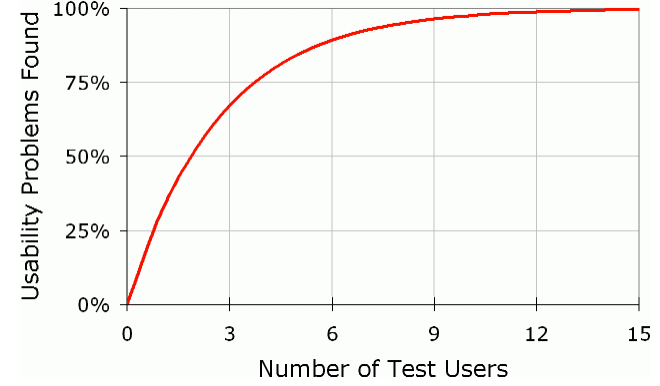
\includegraphics[scale=0.4]{Pictures/app-screenshots/numberoftests.png}
 		\caption{Number of users needed to find percentage of errors according to J. Nielsen\cite{nielsennumberoftests}}
 		 		\label{fig:numberoftests}
 \end{figure}


Nielsen states that after five user tests, 85\% of the errors have been found\cite{nielsennumberoftests}. Molich\cite{molich2008usable} states that six test persons is the ultimate number. Faulkner\cite{faulkner2003beyond} states that while six test persons \textit{may} find 85 \% of the errors, they may also find considerably less. In Faulkner's research, a number of five test users found between 55 \% and 100 \% of the errors, while 20 test persons found between 95 \% and 100 \% of the errors. 

In addition to the practical usability tests, we will use techniques such as background interviews, focus groups and on-site observations. The interviews will be performed in order to achieve a set of control data we can use for comparison when performing later usability test and codesign sessions. As mentioned in \ref{sec:codesign}, we plan on arranging focus group sessions at an early and mid stage of the development of our TUI. These sessions will help us develop our TUI and eliminate usability issues at an early stage. We also plan on using the technique of on-site observation by letting children operate our TUI freely, in order to observe interaction between the children and the TUI. 

\paragraph{Testing environment}
\label{par:testingenvironment}
The next thing to consider when performing usability testing is the testing environment. It should resemble the environment in which the system will be used. To make the most of the tests, it is wise to perform videotaping of the tests. This will help when reviewing the results from the test If the tests are being recorded, a consent from the test person or his/her parent will be required.

Before the test persons arrive, a test leader should be chosen, to guide the test persons through the process. The test leader should be in charge of testing and act as an interviewer to help the participant to ``think-aloud''\cite{lewis1982using}. The test leader should answer questions from the participants, but be careful not to give away information that may affect the results of the test.

After the tasks are done, it is necessary to gather loose ends and obtain answers to all the questions that may remain unanswered. A system usability scale(SUS)\cite{sus} may be a good way to grade the usability of the system together with the observations made during the test. The SUS scale will reflect on how satisfying the usability is in the eyes of the users. Bangor et. al.\cite{susform} have made a scale based on the SUS-forms from different system usability tests, in order to make it possible to compare the mean score of a system with what is an acceptable level of usability. In our testing, we will make use of a Norwegian version, developed by Svan\ae s (see Appendix \ref{app:norsksus}), which will be answered by the test users or the parent of the test user.

\section{How to test usability on children and toddlers}
\label{sec:usabilitytestchildren}
While usability testing on children and toddlers have the same basic approach as testing on adults, there are many more precautions to be followed. 
Hanna et. al.\cite{testingenvironmentforchildren} lays out some of these precautions. They recommend not using children that are skilled with computers since they may find the tasks too easy and will not produce useful data. 
Since children these days have a higher skill with computers thanks to the invasion of tablets and smart phones\cite{babiesusageoftablets}, this may not be great of a concern. 

Since our application is targeted at children with asthma, we want to test the system on children suffering from asthma in addition to children from the same age group, not suffering from asthma. These children will most likely have a different approach to the system and may give different feedback.

Hanna et. al. also point out changes that should be made to the testing environment as mentioned in \ref{par:testingenvironment}. They recommend making the testing environment more suitable for children by placing colourful posters on the walls.
Children of young age may be afraid of ``the Doctor's Office'' and we will need to make adjustments to avoid frightening the children upon their arrival at the test lab. 

As mentioned by Donker and Markopoulos\cite{TalkAloud} talk-aloud is very useful technique when doing usability testing with children. Talk-aloud is a technique were the children talk about what they are doing instead of what they are thinking.

Zaman et. al. proposes a way to measure the likeability of tangible interaction with preschoolers\cite{zaman2007measure}. They based their research on work done by Read, MacFarlane and Casey \cite{read2002endurability}, who found that traditional measures for likeability, for instance a smileyometer, proved to give false results. In fact, Read et. al. found that more than 80\% of the children being tested gave a ``Brilliant'' score. Zaman et. al. implies that children are actually lying when giving these scores, which is understandable from a questionnaire perspective. Instead of using scales as a measure of what is likeable or not, they propose a model where they compare different interaction systems against eachother. They call it the ``This or that'' method. For instance, the interviewer asks the child which system the child prefers, followed by ``this or that'' while pointing to the different systems. We will use a similar approach to understand which forms of interaction children like most.  


\section{Usability testing on mobile devices}
\label{sec:usabilitytestonmobiledevices}
We plan on doing usability testing in testing lab or quiet testing office. The application's main environment for use will be at the user's home, which may be noisier and more hectic than our testing lab. Kaikkonen et. al. states that the similarity between testing environment and place of use is not too important, the test user will still be able to complete the tasks and find the same number of errors cite{kallio2005usability}. This claim is supported by Beck et. al. who discovered that the test persons found more usability problems when sitting down, compared to when walking on the street\cite{beck2003experimental}. 

Schusterich et. al.\cite{schusteritsch2007towards} published a guide on how to build the perfect infrastructure for usability testing on mobile devices, in 2007. They describe how generic infrastructure issues, mobile device-specific issues and usability study context issues should be taken into consideration. Shcusterich et. al. recommends having a number of cameras recording from different angles in order to capture unbiased interaction patterns of the mobile device. 

\subsection{Emulator versus device}
When developing for mobile devices such as Android, it is possible to run an emulator on a pc, instead of running the application on an Android device. The emulator emulates the use of a mobile device on screen. Input must be given by mouse-clicks on buttons/screen elements. The Android emulator emulates use of system resources corresponding to a given Android device, in order to not act faster or slower that a real device. While this may be true in theory, it is not always true in practice. The emulator is often much slower than an actual device.


\begin{figure}
\begin{center}
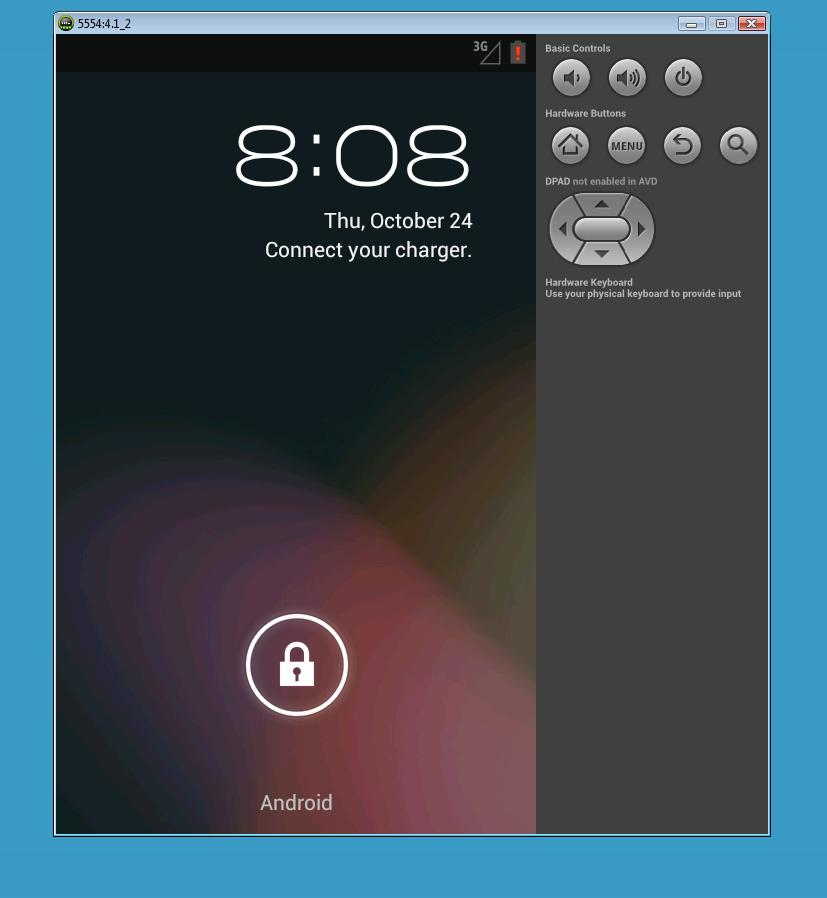
\includegraphics[scale=0.4]{Pictures/app-screenshots/androidemulator.png}
\end{center}
\caption{The Android Emulator running an emulation of Android 4.1}
\label{fig:androidemulator}
\end{figure}

The question arises, should one do usability testing on an emulator or on a real device?
Using the emulator allows for easier capture of the interaction with the device, since it allows screen recording of user input and easier capture of the user when interacting with the emulator. Using a computer as a test object may be more positively perceived by the test user rather than installing the test application on their device or having them doing tests on our device. 

Using a real device has the benefit of being an actual device, and may lead to a more realistic interaction pattern when using the application. While a number of screen recorders for Android devices exist, these require that the device is rooted\fnurl{Android Rooting}{http://en.wikipedia.org/wiki/Android\_rooting} , which is not an option for us. 
The use of a real device also allows the use of gestures, which is a benefit in contrast to the emulator which can simulate swiping. 


Beitol and Cybis\cite{betiol2005usability} compared doing usability testing on a tripod-mounted device to an emulator and using a device in the field. They found that many users found the tripod-mounted device difficult and unnatural to operate. The users found 80\% of the usability issues on the emulator, but Beitol and Cybis points out that use of an emulator may depend on the similarity between the emulator and the device. 

Based on the research we have read we decided to do the usability testing on a real device, in a usability test lab.


\subsection{Introduction to Usability}
\label{sec:introductiontousability}

There are many ways to describe the term usability. 

The International Organization for Standardization(ISO) uses the following definition\cite{isousability}:

\textit{``Extent to which a system, product or service can be used by specified
users to achieve specified goals with effectiveness, efficiency
and satisfaction in a specified context of use.''}

The same document defines the term ``context of use'' as:

\textit{``Users, tasks, equipment (hardware, software and materials), and
the physical and social environments in which a product is used.''}

These definitions cover how the system is used, the user's thoughts about the use and the context of the system. This can be broken down further into several subgoals in order to achieve better usability, and to give a better insight as to what usability is. 
These subgoals are:

\begin{enumerate}
\item{How precisely is the user able to perform a task by using the application?}
\item{How much resources (for example time, or number of tries) was used to perform the given task using the application?}
\item{How many errors occurred?}
\item{Did the user find the use satisfactory?}
\end{enumerate}

Schneiderman stated eight golden rules in order to achieve a good usability of computer systems\cite{shneiderman2003designing}. In his rules he mentions consistency, informative feedback, reducing short term memory load and permitting easy reversal of actions. These eight golden rules have since their publication become a central part of usability engineering.

Today usability is extremely important in order to achieve success for a system. The users expect a functional and easy-to-use system. From the user's point of view, working with a product which is easily understood, leads to increased productivity, which again may lead to increased sales/usage\cite{folmer2004architecting}. Proper usability engineering may also lead to lower costs for the developers and higher chances for projects being finished on time\cite{nielsen1994usability}. 

\subsection{Purpose}
\label{sec:usabilitypurpose}
Usability tests are usually performed in order to detect errors in a system. We wanted to perform usability tests in a slightly different manner. In addition to discover errors, we observed how children take their medicine in combination with technology. We used the results of the usability tests to find potential for improvements and design ideas for the product, in addition to validate whether or not our concept worked in a satisfactory manner.
 
The tasks given to the participants were created with routine use of the application in mind. Usability tests were performed with the help of participants with no prior knowledge of the application. These participants were chosen in order to receive valuable feedback on usability problems with the current design and structure, and to prevent invalid feedback from users who already know how to perform the tasks. In addition, this situation resembled everyday life of the users.

As one of the systems we tested was an Android application, the question of whether we should test it on an emulator installed on a computer, or by the use of a smartphone was raised. While the emulator allows for easier screen and input capturing, it suffers from the drawbacks that interaction is performed through a mouse and a keyboard, in addition to running far slower than an Android device. Using an Andriod device would lead to a more realistic interaction pattern, but it suffers from the drawback that screen capturing is not possible unless the device is rooted\fnurl{Android rooting}{http://en.wikipedia.org/wiki/Android\_rooting}. We chose to test the system on an Android device, as we figured it would seem more natural for a child and the NSEP laboratory has capabilities to record the user interaction through cameras.  


\subsection{Test Method}
\label{sec:testmethod}

The usability tests were performed at the NSEP Usability Lab\fnurl{NSEP Usability Lab}{www.ntnu.no/nsep}, which provided measures for recording the sessions.  

Before each test, we performed a pilot test in order to discover last minute critical errors that could make an impact on the result.

The test was divided into two stages. In the first stage, the parent were to use \app{} for a couple of basic tasks. In the second stage, the child was to perform a set of tasks (the tasks can be found in Appendix \ref{app:scenarioandtasks}). We wanted children to observe while their parent performed the tasks, in order for them to understand that the process was harmless. Additionally, we let their parents sit next to them and explain the tasks for them, such that the children were not told to perform some seemingly random task by a stranger.    
 
The participants were given an Android mobile device to perform their tasks on. The different tasks were given one by one. The participants were introduced to the ``think-aloud''-method\cite{lewis1982using}, and was told to ask questions during the process, even though the test leader was not allowed to answer questions during the test. The main reason for gathering questions was for the discussion afterwards and facilitate for the ``think-aloud''-method. 

The test leader finished the test by asking questions regarding what the participants thought of the system and by answering the questions that were asked during the test. We also asked parents how they felt that the medication process went, so that they could compare it to their daily situation at home, and if they got the impression that the product could be helpful.  

The results were later analyzed in order to discover any improvements needed to the system. The errors were rated after level of severity\cite{dumas1995practical}. 

\begin{itemize}
\item{Critical (Level 1) - Prevents the participant from completing the task.}
\item{Significant (Level 2) - Generates significant problems when trying to complete the task.}
\item{Minor (Level 3) - Has minor effect on the usability of the application.}
\item{Non-essential (Level 4) - Enchancements to the system. When a participant states that ``it would be nice to have this''.}
\end{itemize}


An often used approach to measure the usability of a system, is to use the System Usability Scale (SUS)\cite{sus}, together with the observations made during the test. These scores may give an indication of the usability of a system\cite{susform}. As we were dealing with children, we had to use a different approach in order to get feedback from the children. 

Zaman et. al. proposes a way to measure the likeability of tangible interaction with preschoolers\cite{zaman2007measure}. They based their research on work done by Read, MacFarlane and Casey\cite{read2002endurability}, who found that traditional measures for likeability, for instance a smileyometer, proved to give false results. In fact, Read et. al. found that more than 80\% of the children being tested gave a ``Brilliant'' score. Zaman et. al. implies that children are actually lying when giving these scores, which is understandable from a questionnaire perspective. Instead of using scales as a measure of what is likeable or not, they propose a model where they compare different interaction systems against eachother. They call it the ``This or that'' method\cite{zaman2007measure}. For instance, the interviewer asks the child which system the child prefers, followed by ``this or that'' while pointing to the different systems. We used a similar approach to understand which forms of interaction children like most, and which system they liked to interact with the most, \app{} or \ab{}.   


\subsection{Scenario and Tasks Given to the Users}
\label{sec:scenarioandtasksgiventotheusers}
Since the test users has spoke Norwegian, and some of them were children, the scenario and tasks were given in Norwegian. A translation of the scenario and tasks handed to the participants can be found in Appendix \ref{app:scenarioandtasks}, but for convenience the next paragraphs gives a brief summary.

\textbf{Scenario given to adult test users}

The scenario explained that the user was a parent of a 4-year-old child with asthma. They have recently seen a doctor, and will now have to set up treatment plans according to advice given by the specialist. Since they have little experience with asthma, they would have to look up information about the medicines and how the treatment will be done. In order to motivate the child to continue taking his/her medicine, they will have to add a reward via the application menu. Finally, they would have to look through the calendar log in order to find correlations between the child's health state and the use of medicines. 


\textbf{Scenario given to child test users}

The scenario given to children were explained to them by their respective parents.

The scenario explained that the child needed to take his/her medicine, and that \app{} and \ab{} were there to help him/her through the process. The children started out by checking for potential rewards in \app{}. They then did a treatment with the help of \ab{}, before doing a treatment through \app{}. They were then told to check their amount of stars earned through \ab{}, before they were instructed to purchase their reward from \app{}'s shop.     



%\chapter{First Co-Design Session}
\label{chp:codesignsessionone}

\chapter{Description of [APPNAME]}
\label{chp:description}

This chapter will give a description of [APPNAME], through textual description and screen shots. Please note that the main language of the application is Norwegian, and we have translated parts of it where it seems appropriate. 

\section{Basic System Architecture}
Figure \ref{fig:basic-architecture} shows an overview of the architecture we intend to use for our solution. We will build upon the architecture used by Aaberg et. al. \cite{CustomerDriven}.

We have access to a MySQL-server hosted at NTNU, which we will access by a PHP-server hosted at NTNU. The main reason we have to access the database through a server layer, is that it is quite cumbersome to connect to the database if a device is not connected at NTNU's network. In addition, by having a webservice do some of the work for us, it becomes easier to parse results from the database through JSON.   


The downside by having this approach is that scalability suffers from this architectural choice. However, we consider these problems as outside the scope of our thesis, and will continue using this approach.

\begin{figure}
		\centering
			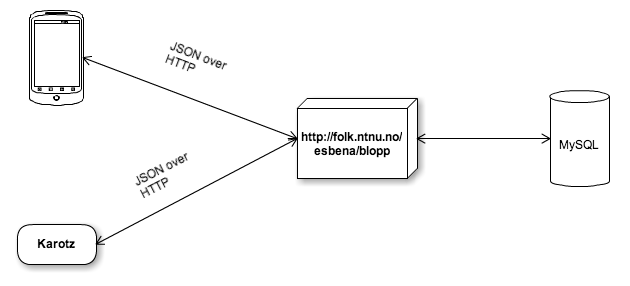
\includegraphics[width=0.50\paperwidth]{Pictures/basic-architecture.png}
		\caption{Basic architecture of our system}
		\label{fig:basic-architecture}
\end{figure}

\section{Child partition}
\label{sec:description-child-partition}
The child partition of our application consists mainly out of four parts. When Aaberg et. al. created the original application, they wanted a conceptual look and feel throughout the applications. They used images of Karotz in the application in order to introduce a sense of completeness, i.e. the Karotz bound CAPP, GAPP and KAPP together. [TODO: Vi burde bytte ut Karotz-bilder med eget produkt imo]. 

\subsection{Treatment}
\label{sec:sec:description-treatment}
Figure \ref{fig:capp_start_treatment} shows a screenshot for the application when the child starts their treatment. Starting this sequence can come from one out of two events: (i) \emph{The child reacts to an alarm set in the guardian partition}, and (ii) \emph{The child needs to take their medicine by need}. If (ii) is the case, the child is instructed to pick the medicine from a list shown by the application. If (i) is the case, the medicine is chosen beforehand. When a child has started their treatment, they are taken through an animated sequence, which reacts when a child interacts with the device. In addition, they are being told what to do through the comforting voice of Yngve Svalestuen.  


\subsection{Showing rewards}
\label{sec:description-show-rewards}
Figure \ref{fig:capp_stars} shows a screenshot for the application when the child wants to review how many stars he/she has received, based on the amount of medicine they have taken. We have made two design decisions for our reward system. First, we never want stars to be removed. We don\'t want children to feel that credits are being removed from them. Second, we can\'t assume children are able to read, and thus we have made it countable, and hopefully they can comprehend how many stars they've actually got. In addition, we provide some help to those who are able to read numbers, by showing the amount of stars a child has on the top. The downside here comes when a child has been given a huge number of treatment, such as 200 treatments or more. This will obscure the view.     

\subsection{Shop}
\label{sec:description-shop}
In the shop, children are allowed to buy rewards from parents [Insert Reference]. Figure \ref{fig:capp_store} shows a inside-view of our shop. Children can buy an activity by pressing the selected activity. Due to time constraints, we have not been able to implement voice over, so the children will have to find a parent who can read it if they are not able to [TODO: 1: Bryter med linjen over. 2: Implementasjon av voice over med norsk som språk er vanskelig]. 



\subsection{Treatment instructions}
\label{sec:description-instructions}
The treatment instructions is a book-styled instruction set which shows generically how to take a medicine. 
The following steps are included in instructions: 
\begin{enumerate}
  \item Shake the inhaler such that the particles loosen up. 
  \item Take the cap of the inhaler
  \item Attach the inhaler to the inhaling chamber [TODO: Korrekt bruk av chamber?]
  \item Put the inhaler onto the face of the child
  \item Press the inhaler until you hear a sound
  \item Let the child breathe calmly 10 times in and out
  \item Let the child wash his/her mouth
\end{enumerate} 



\begin{figure}
	\begin{minipage}[b]{0.4\linewidth}
		\centering
			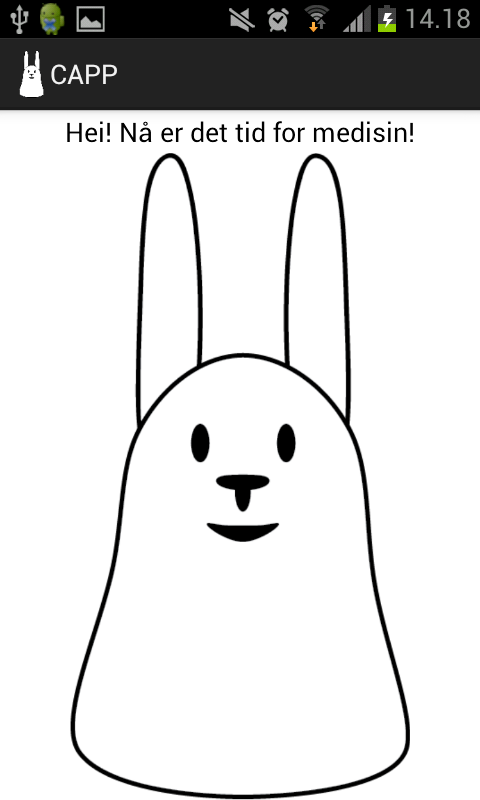
\includegraphics[width=0.20\paperwidth]{Pictures/app-screenshots/capp_start_treatment.png}
		\caption{Starting a treatment}
		\label{fig:capp_start_treatment}
	\end{minipage}
	\hspace{3cm}
	\begin{minipage}[b]{0.4\linewidth}
		\centering
			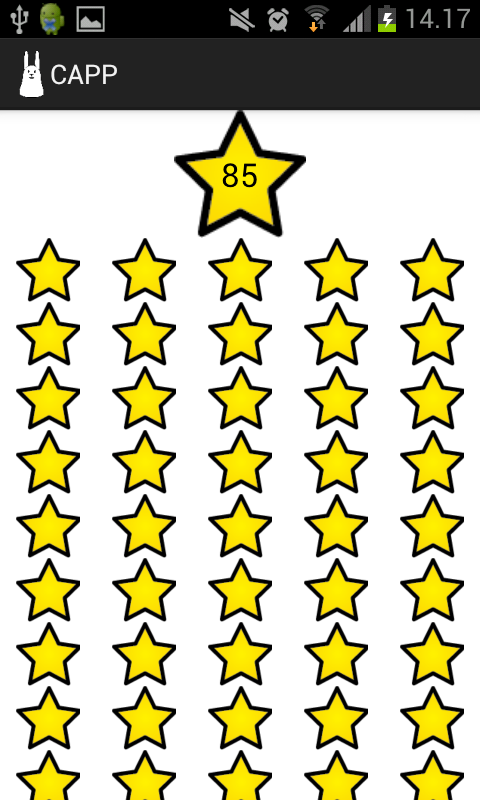
\includegraphics[width=0.20\paperwidth]{Pictures/app-screenshots/capp_stars.png}
		\caption{SHOULD BE A SHOP}
		\label{fig:capp_store}
	\end{minipage} 
\end{figure}

\begin{figure}
	\begin{minipage}[b]{0.3\linewidth}
		\centering
		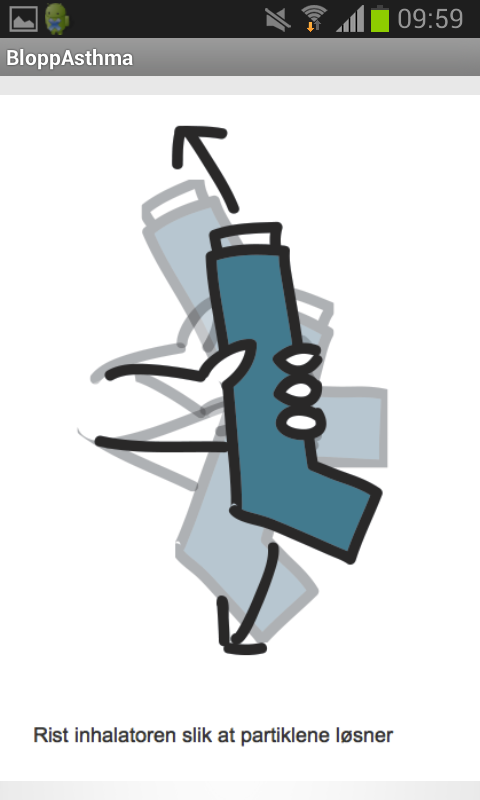
\includegraphics[width=0.20\paperwidth]{Pictures/app-screenshots/instructions-1.png}
		\caption{Instructions 1}
		\label{fig:instructions-1}
	\end{minipage}
	\begin{minipage}[b]{0.3\linewidth}
		\centering
		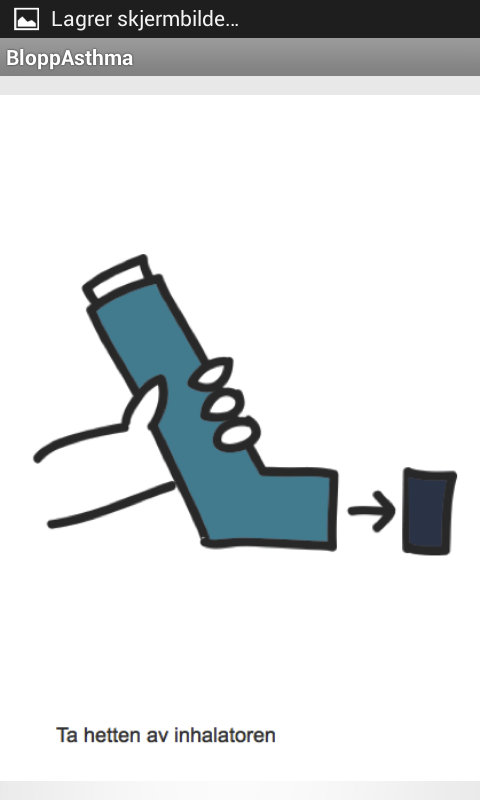
\includegraphics[width=0.20\paperwidth]{Pictures/app-screenshots/instructions-2.png}
		\caption{Instructions 2}
		\label{fig:instructions-2}
	\end{minipage}
	\begin{minipage}[b]{0.3\linewidth}
		\centering
		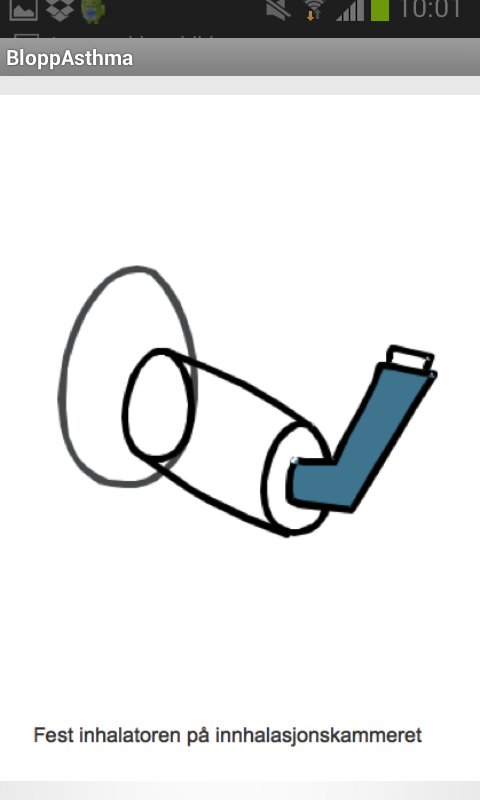
\includegraphics[width=0.20\paperwidth]{Pictures/app-screenshots/instructions-3.png}
		\caption{Instructions 3}
		\label{fig:instructions-3}
	\end{minipage}
	
	\begin{minipage}[b]{0.3\linewidth}
		\centering
		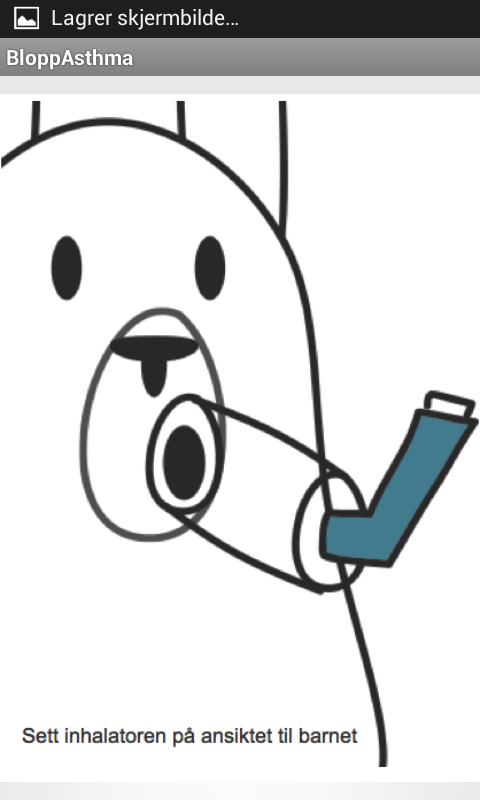
\includegraphics[width=0.20\paperwidth]{Pictures/app-screenshots/instructions-4.png}
		\caption{Instructions 4}
		\label{fig:instructions-4}
	\end{minipage}
	\begin{minipage}[b]{0.3\linewidth}
		\centering
		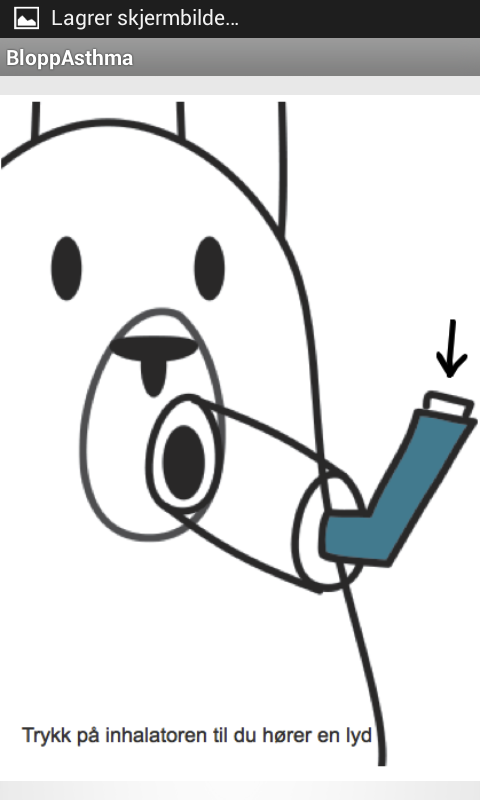
\includegraphics[width=0.20\paperwidth]{Pictures/app-screenshots/instructions-5.png}
		\caption{Instructions 5}
		\label{fig:instructions-5}
	\end{minipage}
	\begin{minipage}[b]{0.3\linewidth}
		\centering
		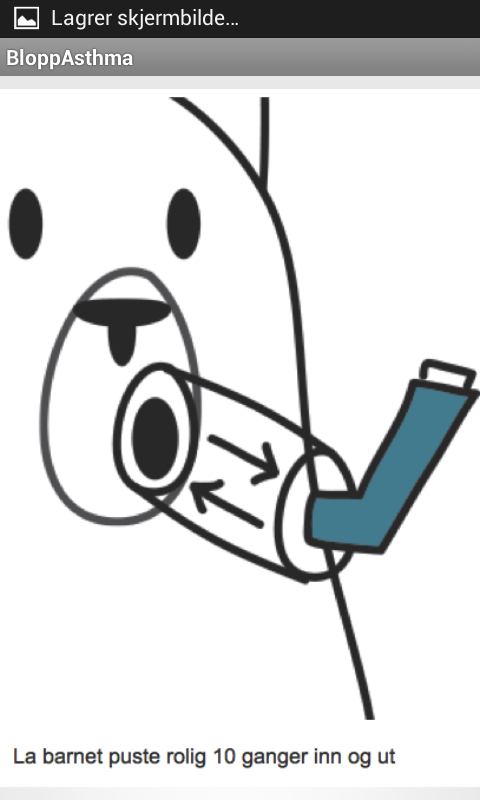
\includegraphics[width=0.20\paperwidth]{Pictures/app-screenshots/instructions-6.png}
		\caption{Instructions 6}
		\label{fig:instructions-6}
	\end{minipage}
	
	\begin{minipage}[b]{0.3\linewidth}
		\centering
		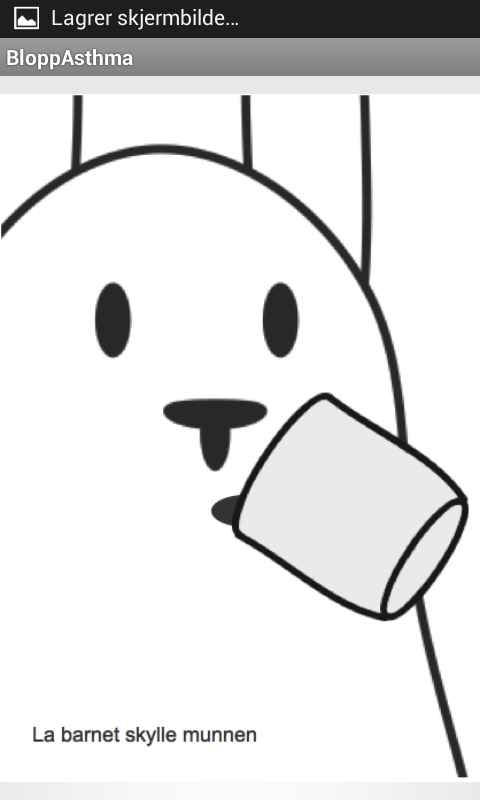
\includegraphics[width=0.20\paperwidth]{Pictures/app-screenshots/instructions-7.png}
		\caption{Instructions 7}
		\label{fig:instructions-7}
	\end{minipage}
\end{figure}





\section{Guardian partition}
This section will take you through the Guardian partition of [INSERT APPNAME].

\subsection{Menu}
\label{sec:description-menu}
Figure \ref{fig:gapp-main-menu} shows the main menu of the guardian partition. It has six options (norwegian translation in paranthesis):
\begin{enumerate}
  \item Medicine Plan (\emph{Medisinplan})
  \item Register Medicine Afterwards (\emph{Etterregistrer medisin})
  \item Medicine Log (\emph{Medisinlogg})
  \item Medicine Information (\emph{Legemiddelinformasjon})
  \item Manual (\emph{Manual})
  \item Rewards (\emph{Premier})
\end{enumerate} 


\subsection{Medicine plan}
\label{sec:description-medicine-plan}
Creating a medicine plan for asthma treatment is highly connected to the Traffic Light System [INSERT REFERENCE].
Users can have three different plans, depending on which health state they are currently in. As we are targeting children, we can not assume that they are aware of which category they are currently in, and as a result, we let their guardians control it. Figure \ref{fig:gapp-view-plans} and [INSERT REFERENCE TO EDIT PLAN] shows the view in which one may the change medicine plan their child are currently on, in addition to setting alarms where appropriate. For instance, one might set an alarm at 07:00, which makes the user aware before it is time to leave for school. Changing medicine plan is done by selecting the checkbox at the left side of the panel.  

\subsection{Register medicine}
\label{sec:description-register-medicine}
What happens if a child need their medicine, but the application or our TUI is not nearby? They would probably be mad because they did not get their star, and did not make any progress as far as the rewards go. Fortunately, it is possible to register a medicine that has been taken afterwards, which entitle the child the amount of stars they should have gotten. \emph{Register Medicine Afterwards} allows parents to register the medicine, at any given day prior to current time (See Figure \ref{fig:gapp-register-treatment}).  


\subsection{Medicine log}
\label{sec:description-medicine-log}
The \emph{Medicine log} can be used by parents to show how many times a child has taken their medicine. One of the main reasons that children does not take their medicine is lack of communication between parents. Having an option to show medicine log, give parents the ability to check and see whether they have taken the necessary amount at a given day.

Figure [INSERT REFERENCE] shows the calendar view of the application. The view is a bit complicated, and an explanation is in it's place. We'll start out by the cells in the calendar. They obviously show any given day of a month. In addition, there is a top bar in the view. The top bar indicates which health state (or health plan) the child was in at a given day. At the bottom of the screen, there are three panels. The left one shows which medicine that has been taken at a selected day. The middle one shows the air quality in Trondheim. The right shows the pollen distribution of the 6 most common pollen types. The idea behind this is that asthma symptoms can often be the same as allergy symptoms, and if guardians are able to recongize a pattern between health state and pollen distribution, they might want to take their child to a hospital.   
 
\subsection{Medicine information}
\label{sec:description-medicine-information}
Figures \ref{fig:information-1} and \ref{fig:information-2} shows the application's medicine information functionality. The information part of the application is a part that is somewhat down-prioritized. At the time being, it contains a lightweight description of what it is, what it is used for, important information and how you apply it. 


\subsection{Manual}
\label{sec:description-manual}
The manual contains excactly the same information as shown in Section \ref{sec:description-instructions}. [TODO: Beskrive hvorfor dette er to steder i appen?]


\subsection{Reward}
\label{sec:description-manage-rewards}
Figure \ref{fig:reward-list} shows the list of possible rewards a child might receive. They are added by parents through \emph{Add reward}. The idea of having guardians set their children's rewards is to specify rewards according to children's interest [TODO: Referanse til hvor vi har sagt dette før]. Figure \ref{fig:add-reward} shows how one may add an activity. Users inserts a description, then either take a photo or select one out of our standard images. It is possible to set a reward on ``Repeat'', which will make the reward repeating with twice the amount of stars [TODO: Omformuler].        
When the user press \emph{Save} (Lagre), the reward is added and children have the possibility to buy it. 
 

\begin{figure}
	\begin{minipage}[b]{0.3\linewidth}
		\centering
		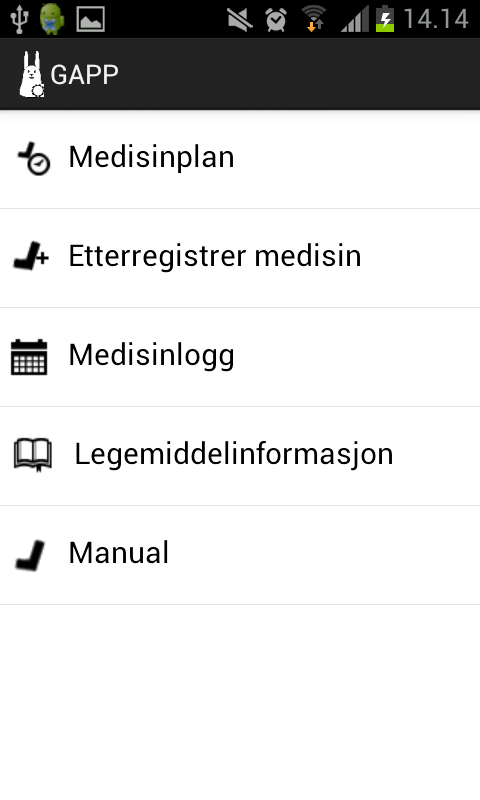
\includegraphics[width=0.20\paperwidth]{Pictures/app-screenshots/gapp_main_menu.png}
		\caption{Menu in guardian partition}
		\label{fig:gapp-main-menu}
	\end{minipage}
	\begin{minipage}[b]{0.3\linewidth}
		\centering
		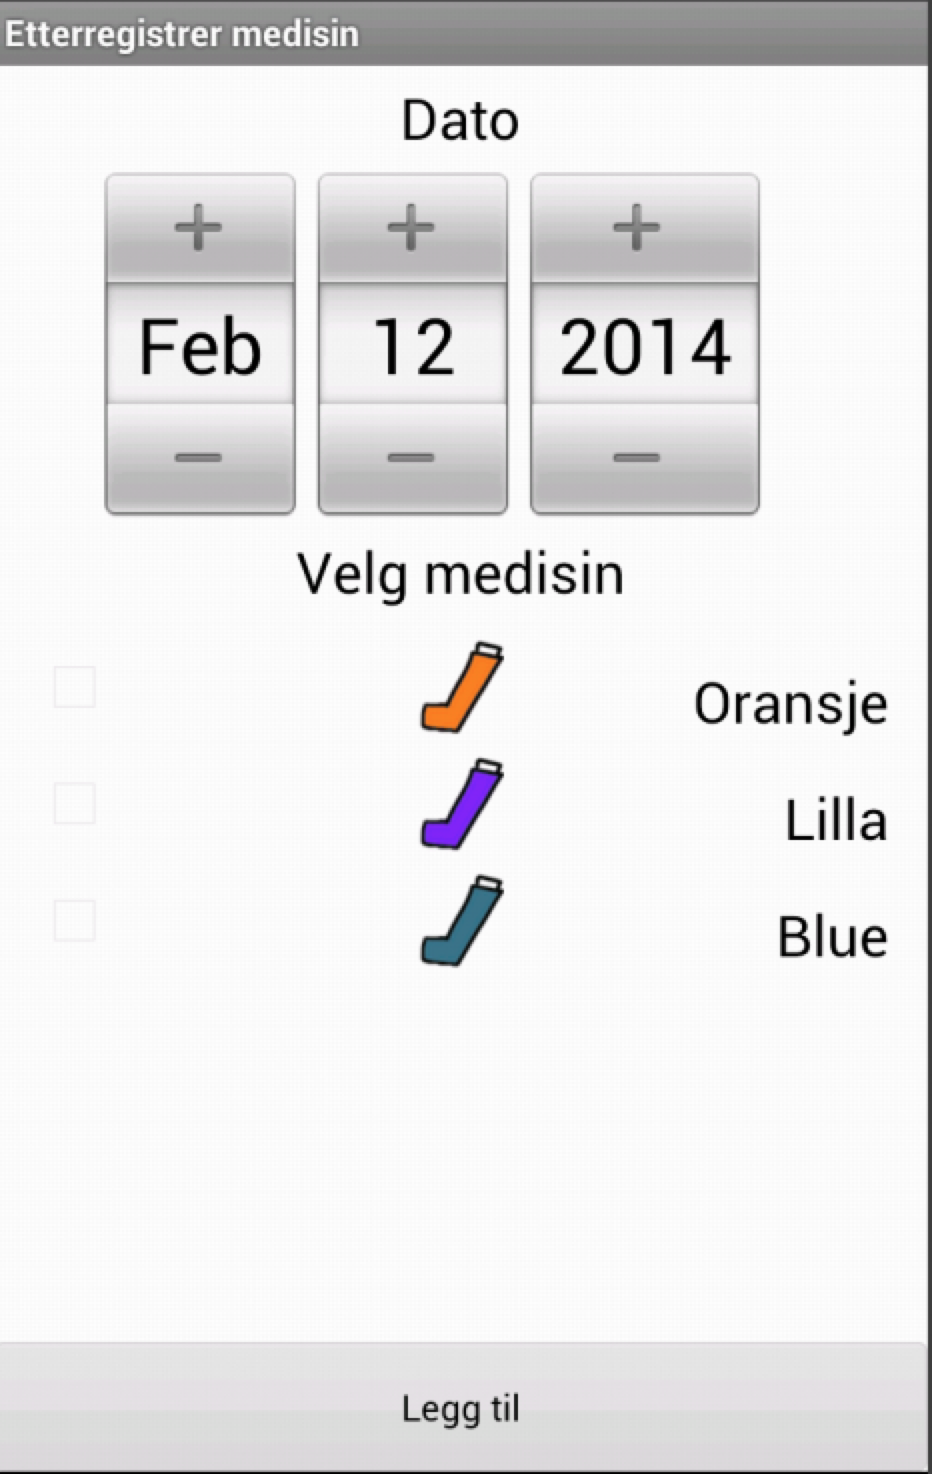
\includegraphics[width=0.20\paperwidth]{Pictures/app-screenshots/register_treatment.png}
		\caption{Register treatment}
		\label{fig:gapp-register-treatment}
	\end{minipage}
	\begin{minipage}[b]{0.3\linewidth}
		\centering
		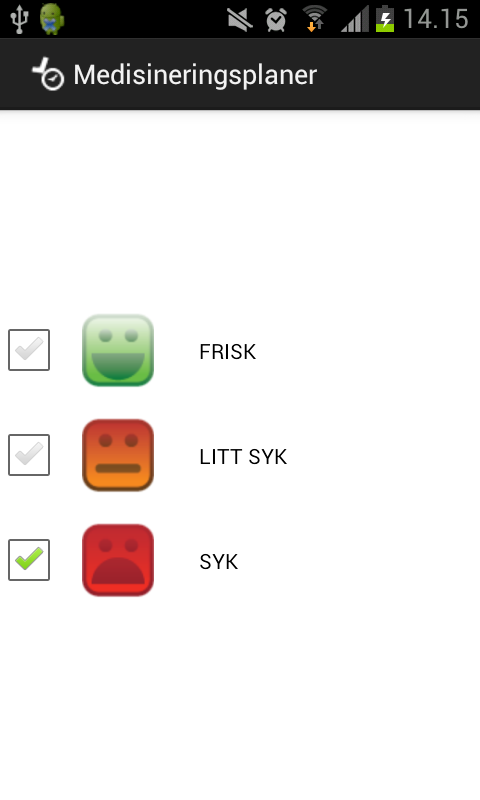
\includegraphics[width=0.20\paperwidth]{Pictures/app-screenshots/gapp_view_plans.png}
		\caption{View plans}
		\label{fig:gapp-view-plans}
	\end{minipage}
	\begin{minipage}[b]{0.3\linewidth}
		\centering
		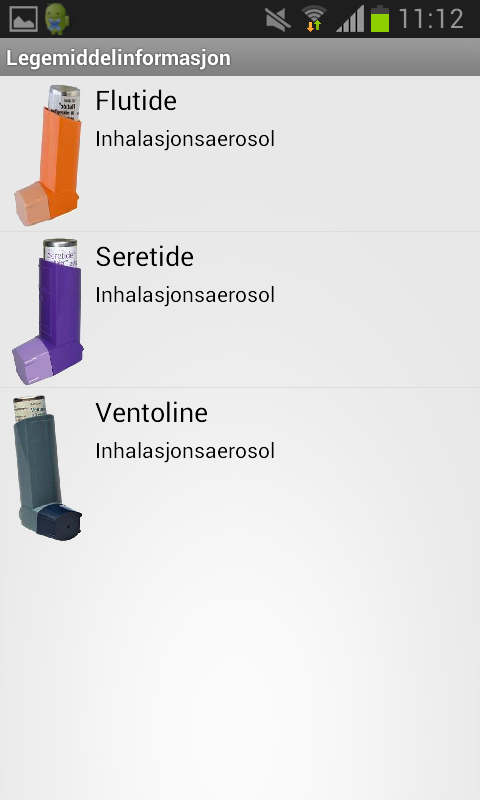
\includegraphics[width=0.20\paperwidth]{Pictures/app-screenshots/information-1.png}
		\caption{Information 1}
		\label{fig:information-1}
	\end{minipage}
	\begin{minipage}[b]{0.3\linewidth}
		\centering
		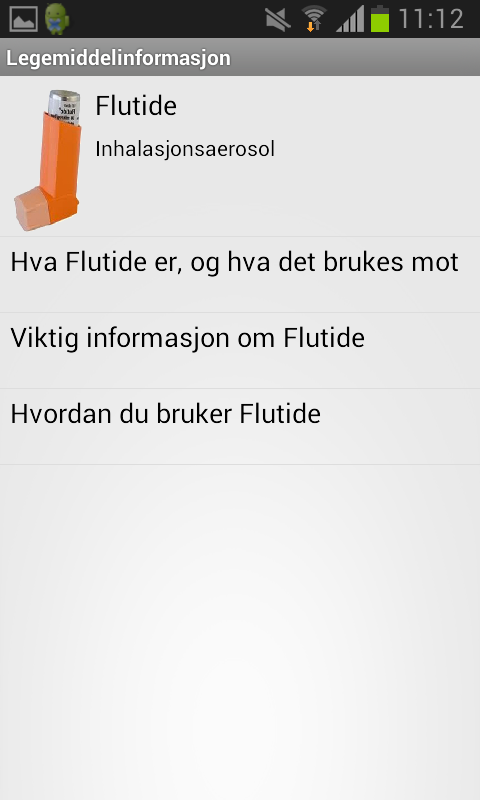
\includegraphics[width=0.20\paperwidth]{Pictures/app-screenshots/information-2.png}
		\caption{Information 2}
		\label{fig:information-2}
	\end{minipage}
	\begin{minipage}[b]{0.3\linewidth}
		\centering
		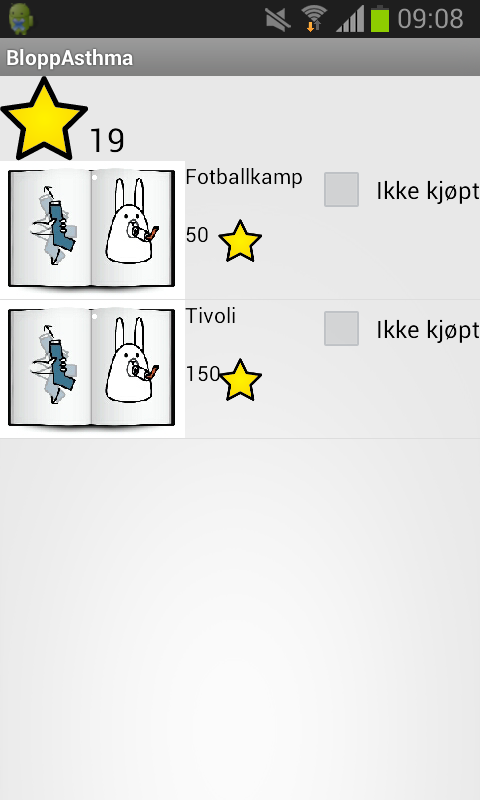
\includegraphics[width=0.20\paperwidth]{Pictures/app-screenshots/reward-list.png}
		\caption{Reward list}
		\label{fig:reward-list}
	\end{minipage}
	\begin{minipage}[b]{0.3\linewidth}
		\centering
		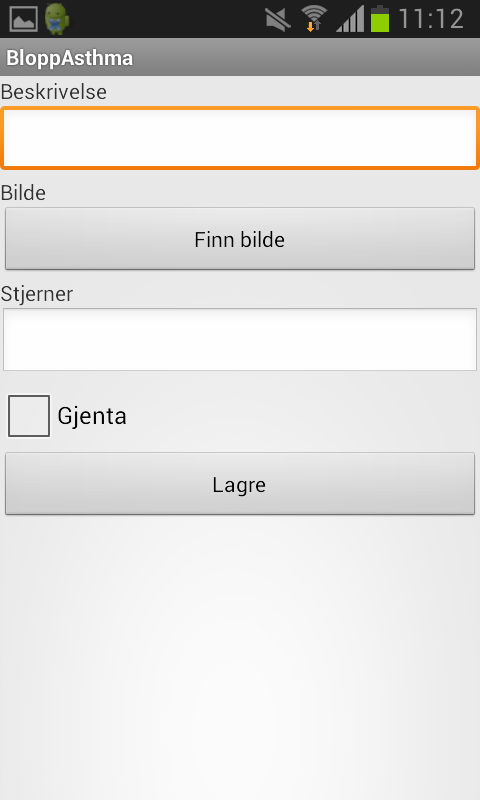
\includegraphics[width=0.20\paperwidth]{Pictures/app-screenshots/add-reward.png}
		\caption{Add reward}
		\label{fig:add-reward}
	\end{minipage}
\end{figure}
% Skjermbilder -> Forklaringer
% Dropper alt som har med Karotz å gjøre, med unntak av ``konsept''-følelsen
% 


\chapter{AsthmaBuddy}
\label{chp:our-solution}

\section{Background}
As mentioned in Chapter \ref{chp:background}; in 2012, we did a similar project using Karotz\fnurl{Karotz}{www.karotz.com} as the platform for the tangible user interface\cite{CustomerDriven}.
This project left us with mixed feelings towards Karotz as a platform. The thought behind Karotz is great. It is an open source robot which allows people to build applications and launch it to the Karotz store. However, in our subjective opinion, it is not ideal to work with. The Karotz starters kit costs ~\$200, not including customs. Thus it is a pretty large investment for a family wanting to use our application. The API is only documented in French, which limits the number of developers who are willing to develop applications for the Karotz, in addition to the fact that it is pretty cumbersome to configure for a ``non-technological'' family. 

We researched other options than Karotz to create our tangible user interface. The alternatives we looked into was Arduino and Raspberry Pi. Arduino is an open source electronics prototyping platform\cite{arduino}, which allows for many different combinations of configurations. Arduino shields comes in many shapes and sizes and is built for modularity and extendability. A wide-range of components are available if you want to add technical functionality to an Arduino system, such as Bluetooth, WiFi or small motors. 
While Arduino allows complex hardware configurations, Raspberry Pi makes larger abstractions, which seemed like the better choice for us as developers. Arduino programs are normally written in C\cite{strahl2000language}, which we had little to no prior experience with. Additionally, Arduinos generally have low-powered CPUs, in order to keep them cheap. These low-powered CPUs tend to have problems with decoding MP3-files, which would lay heavy constraints to our system (without using sounds or a display, it is hard to communicate with children). Due to these facts, we choose to develop the system on a Raspberry Pi.

Our tangible user interface was planned to contain a lot of the same functionality that KAPP had, with some modifications. The reason we chose to develop on a different platform was to make the system more user friendly, specifically lower the requirement for technical knowledge needed to introduce \ab{} to an inexperienced user, by following the ``Plug and Play'' principle.
 
\section{Technology}
\label{sec:technology}

\subsection{Raspberry Pi - Specifications Overview}
The \rpi{} was initially intended to teach british school children about computer programming\cite{rasperrypi-about}. Since its release, it took an unexpected turn when lots of computer enthusiasts bought the product to do their own mini projects for a cheap price. 

The specification of a \rpi{} (Model B) is included in Table \ref{tab:pi-specs}. Figure \ref{fig:pi-arch-overview} shows an overview of the \rpi{}.        

\begin{table}[H]
\centering
\begin{tabular}{|p{6.0cm} | p{6.0cm} |}
\hline 
\textbf{Property} & \textbf{Specification} \\
\hline
CPU & 700 MHz ARM1176JZF-S core \\
\hline
Memory & 512 MB \\
\hline
USB 2.0 ports & 2 \\
\hline
Video Output & HDMI \\
\hline
Audio Output & 3.5 mm jack, in addition to ability to play sound through HDMI \\
\hline
Low-level Peripherals & 8 x GPIO (General Purpose Input/Output) \\
\hline
Power Source & 5 volt MicroUSB \\
\hline
Storage & SD card (available with preinstalled OS) \\
\hline
Network & 10/100 Mbps Ethernet  \\
\hline
\end{tabular}
\caption{Raspberry Pi specifications}
\label{tab:pi-specs}
\end{table}

\begin{figure}[H] 
	\begin{minipage}[t]{0.4\linewidth}
	\centering
		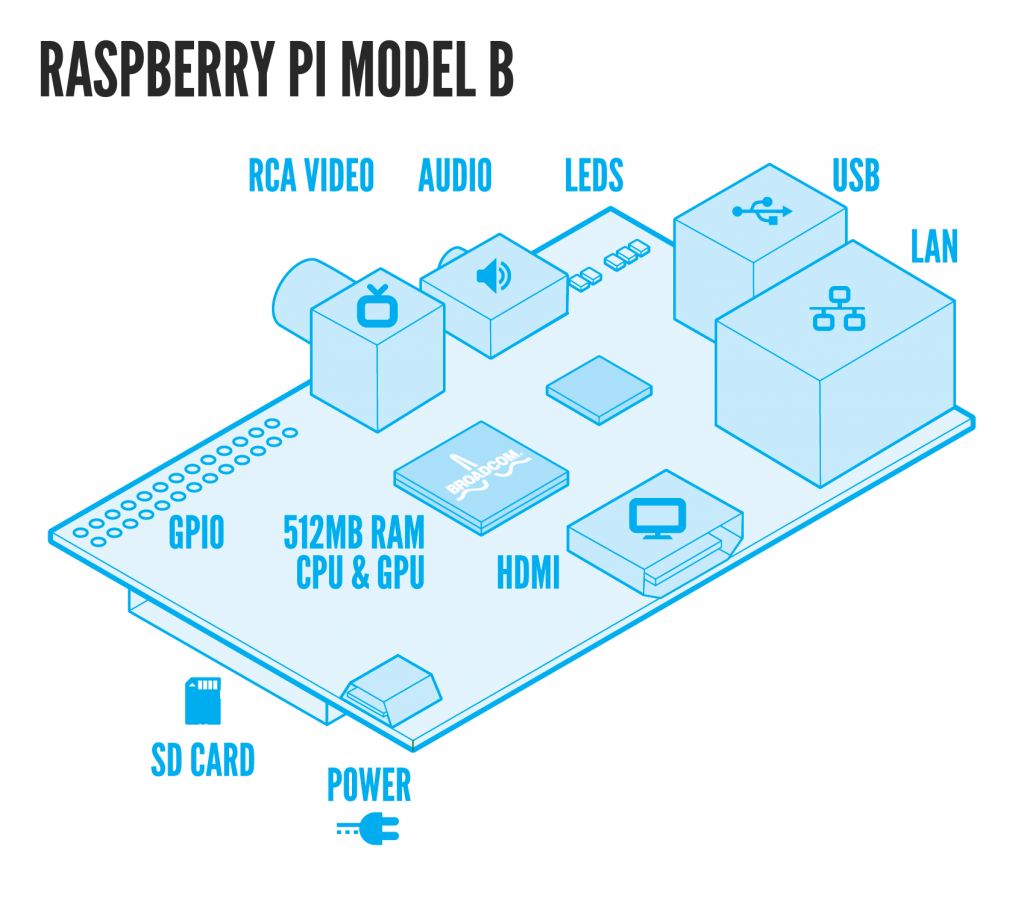
\includegraphics[width=0.3\paperwidth]{Pictures/rpi-arch-overview.png}
	\caption[Raspberry Pi Model B Architecture]{Raspberry Pi Model B architecture.}
	\caption*{Image source: \url{http://raspberrypi.org/faqs}}
	\label{fig:pi-arch-overview}
	\end{minipage}
	\hspace{2.0cm}
	\begin{minipage}[t]{0.4\linewidth}
		\centering
			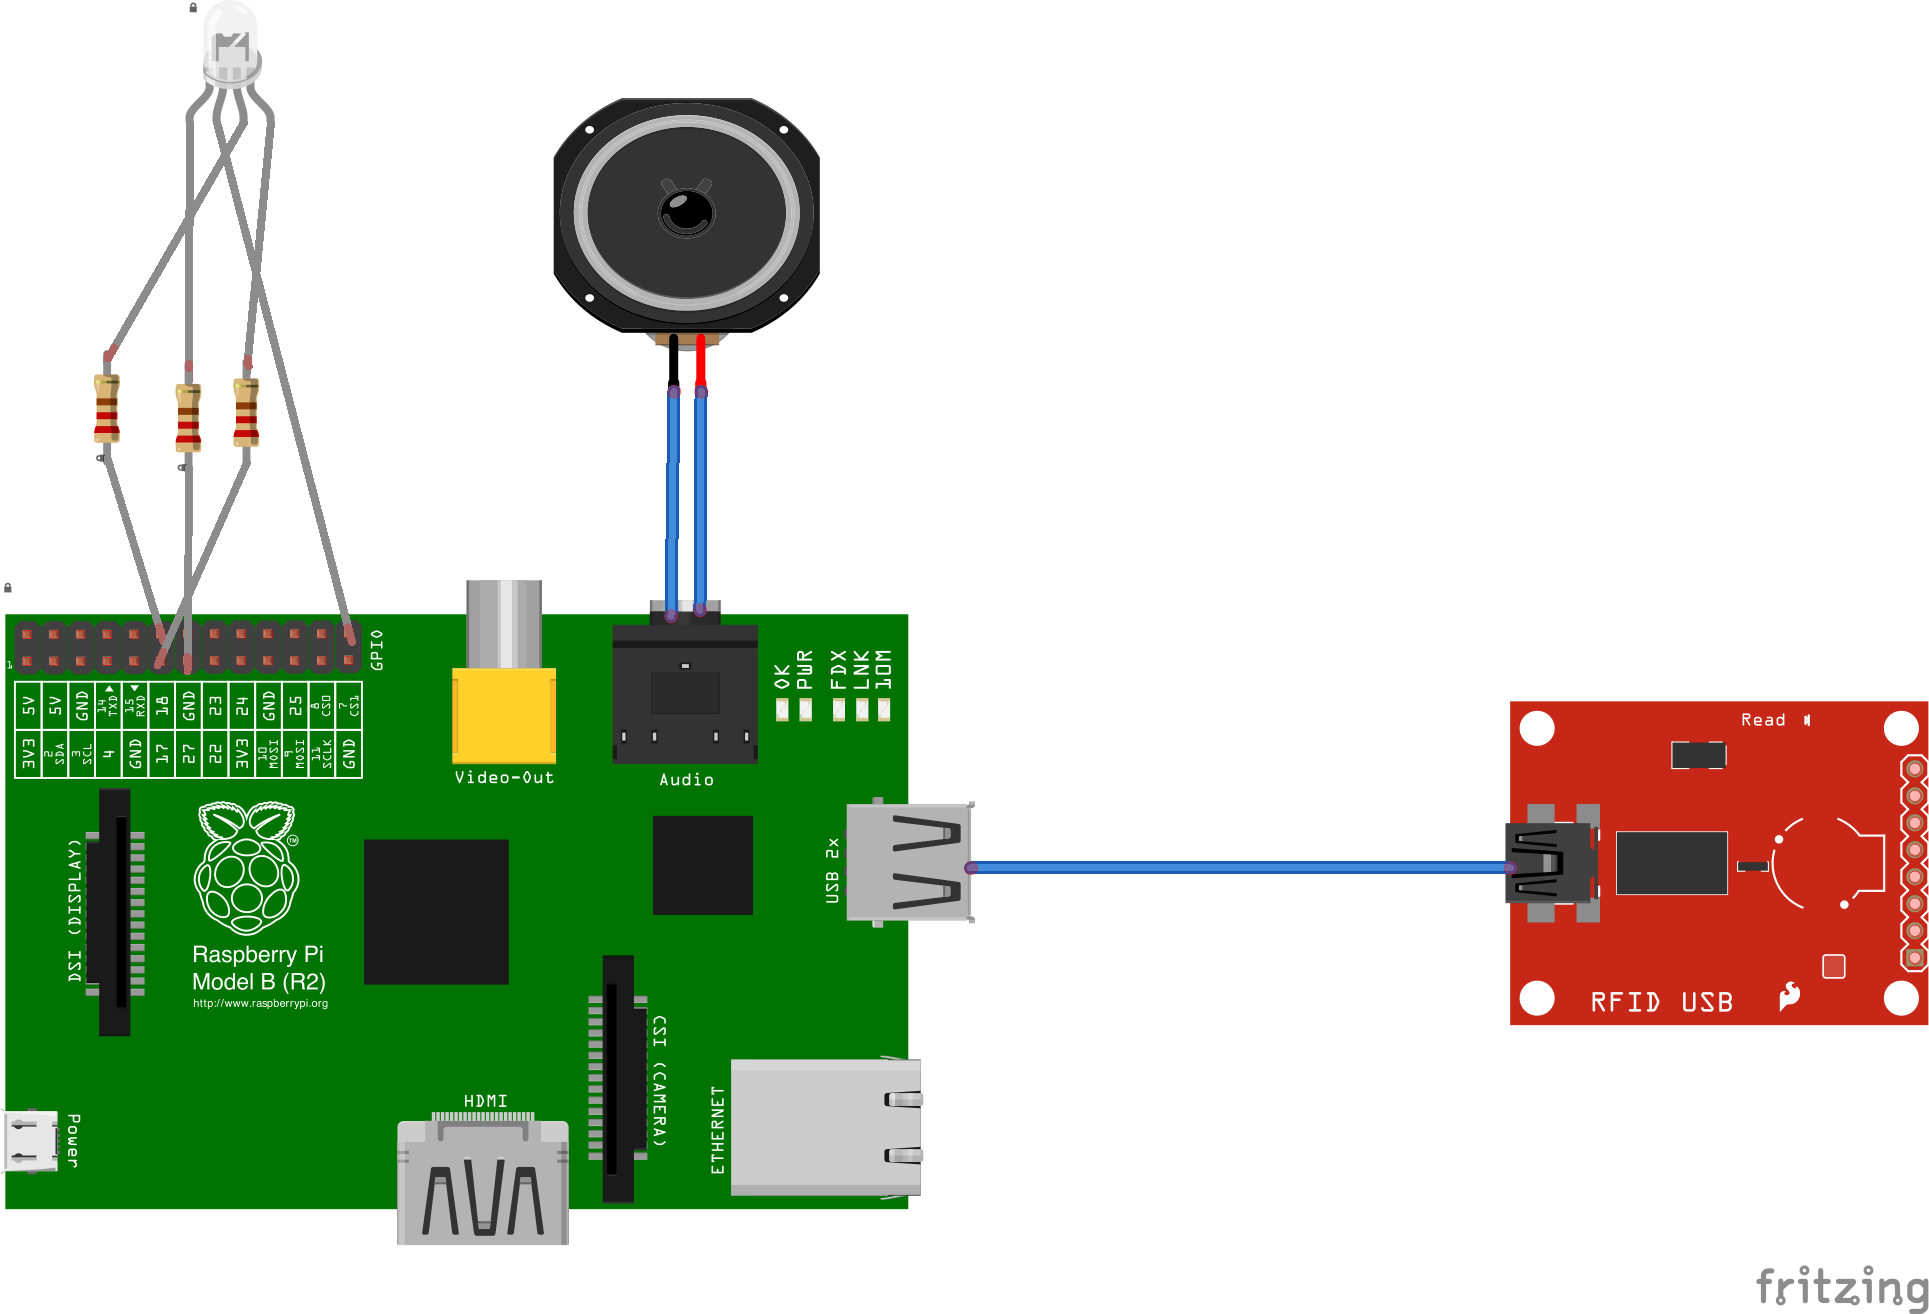
\includegraphics[width=0.3\paperwidth]{Pictures/pi-fritzing-model.png}
		\caption{Digital schematic of the components}
		\label{fig:pi-fritzing}
	\end{minipage}
\end{figure}
 
  
\subsection{Additional Components}
\label{sec:additionalcomponents}
In addition to the \rpi{} we needed some components that children are able to interact through. These components and their functionality are summarized in this section. 


\textbf{RFID Reader}

In order to interact with \ab{}, children can register RFID-tags against \ab{}'s stomach. The RFID-reader we used was a Sparkfun ID-12LA\fnurl{Sparkfun ID-12LA documentation}{http://tiny.cc/sparkfundoc}. The requirements when choosing the reader was that it should be able to connect through an USB-port, and be able to communicate with UNIX-systems.
         
\textbf{USB speakers}

In order to play sounds to children, we decided to integrate speakers inside AsthmaBuddy. Since we did not want to pull too many wires out of the bear, we decided to use USB-powered speakers.    


\textbf{LED lights}

We used LED lights connected to a breadboard in order to play around with the first prototype. The LED lights emits light in different colors to correspond to what action(s) is expected from the user during a treatment (see more in \ref{sec:proto1}). 

In order to display the correct colors to the children, according to the color of the medicine, we tried to use PWM\fnurl{Pulse-width Modulation}{http://en.wikipedia.org/wiki/Pulse-width\_modulation}. However, these experiments resulted in a significant weaker light. Thus, we used a simple combination of Blue and Red in order to show purple, and a combination of Red and Green to show orange.  

 
Figure \ref{fig:pi-fritzing} shows a digital overview of \buddy{}. The green figure to the left is our \rpi{}. While it is also connected to a power supply and an internet cable, we chose not to include these in our figure. The red figure to the right is the RFID reader. It is connected to the \rpi{} through an USB cable. The black figure on top is the speaker, connected to the \rpi{} through the audio port. 
The grey lines and the lamp represents our LED light. It is connected to three of the GPIO (General Purpose I/O) ports on the \rpi{}, through a resistor. The last leg of the LED light is connected to ground on the \rpi{}, without a resistor.

A complete guide for wiring the components and running the application is included in Appendix \ref{app:asthmabuddy_manual}.

\subsection{Components Considered for Use}
\label{sec:componentsconsidered}
In addition to the components mentioned in the last section, we considered using buttons, touch sensors and a microphone. Even though we did not use these components, we simulated them during user tests using the Wizard-of-Oz technique. 

\textbf{Buttons}

One or more buttons could have been used on \ab{}. Buttons could have been used to manage boolean values, for instance if the progression of an instruction needed a yes/no answer. We did not include buttons, as it could disturb the impression of \ab{} as a regular teddy bear, i.e. it would look more mechanical. Additionally, we were not able to restrict the amount of buttons needed. 

\textbf{Touch sensors}

A touch sensor could serve the same purpose as a single button. We did not include this component, as it would require a set of low level programming skills. 

\textbf{Microphone}

A microphone could be used for speech recognition purposes. However, the \rpi{} does not have the processing power required to do speech recognition. Additionally, it would require writing code that is able to distinguish between noises\footnote{We were not able to find any open source libraries that are able to do speech recognition for the Norwegian language}. We thought it could have been a cool feature that would help establishing a relationship between the user and \ab{}.    

\subsection{Frameworks and Libraries Used in \ab{}} 

\textbf{Pi4j}

We wanted to write the code on our \rpi{} in Java, as it was our most familiar programming language. It is, however, cumbersome to use \rpi{}'s GPIO-ports and serial communications with native Java. Pi4j\fnurl{Pi4j}{http://pi4j.com} solved this problem, by making the necessary hardware abstractions.

\textbf{Gson}

Refer Section \ref{sec:techandframeinapp} for a description of Gson.    

\textbf{JLayer}

JLayer \fnurl{Javazoom JLayer}{http://www.javazoom.net/index.shtml} is an open source MP3 decoding library. We used it to play back audio tracks on the \rpi{}. It is an old project, and might be out dated, but it did its job for our purposes.  
 

\section{Design Rationale}
\label{sec:designrationale}
\subsection{Why a Teddy Bear?}
When designing \buddy{} we choose to use a teddy bear as an avatar for our system. There are several reasons as to why we think a teddy bear is an appropriate avatar. Teddy bears are well known toys, and have been loved by children for a long time. They are considered gender-neutral\cite{stagnitti1997determining}\cite{cherney2006gender} and in our subjective opinion it is a toy that could be discretely placed in a child's room. With the appearance of a teddy bear, \buddy{} can easily be placed among other toys and not stand out. It was also important for us to choose a teddy bear of some size. A too thin a bear could lead to problems when fitting the system inside the bear, and could in could be met with scepticism by the children. \buddy{} will have similarities to Tamagotchi\cite{tamagotchi} and Furby\cite{furby}, but \buddy{}'s purpose is to motivate, instruct and teach children about asthma, not be a toy purely for playing with. 

While designing our system we also wanted to make sure that our system did not have robot-like features or robotic similarities. While children tend to find technology very interesting, we wanted to make \buddy{} seem as natural as possible, making a stuffed toy animal, rather than a technological toy. We believe that these design choices served our purpose of making children more aware of their asthma, while not being a constant reminder and a stress element. 

Norwegian fire fighters have used a teddy bear in order to calm down children who find themselves in dramatic situations\fnurl{NRK: Firefighters use teddy bears to calm down children}{http://www.nrk.no/trondelag/bamser-i-utrykningsbilene-1.11548966}. The fire fighters state that the children respond positively to the teddy bear. 
While we were not able to find scientific research done on the use of teddy bears in dramatic situations, we found this news article interesting and worth mentioning in our research. 

A teddy bear has also been used as an avatar for giving instructions on how to apply a treatment correctly. Glaxo Smith Kline, a leading company within consumer health care, uses a teddy bear in their instruction manual for the use of asthma medicine and the breathing chamber\cite{glaxosmithkline}. 

Below are two pictures of how \ab{} looks in its final form. 

\begin{figure}[H] 
	\begin{minipage}[t]{0.4\linewidth}
	\centering
		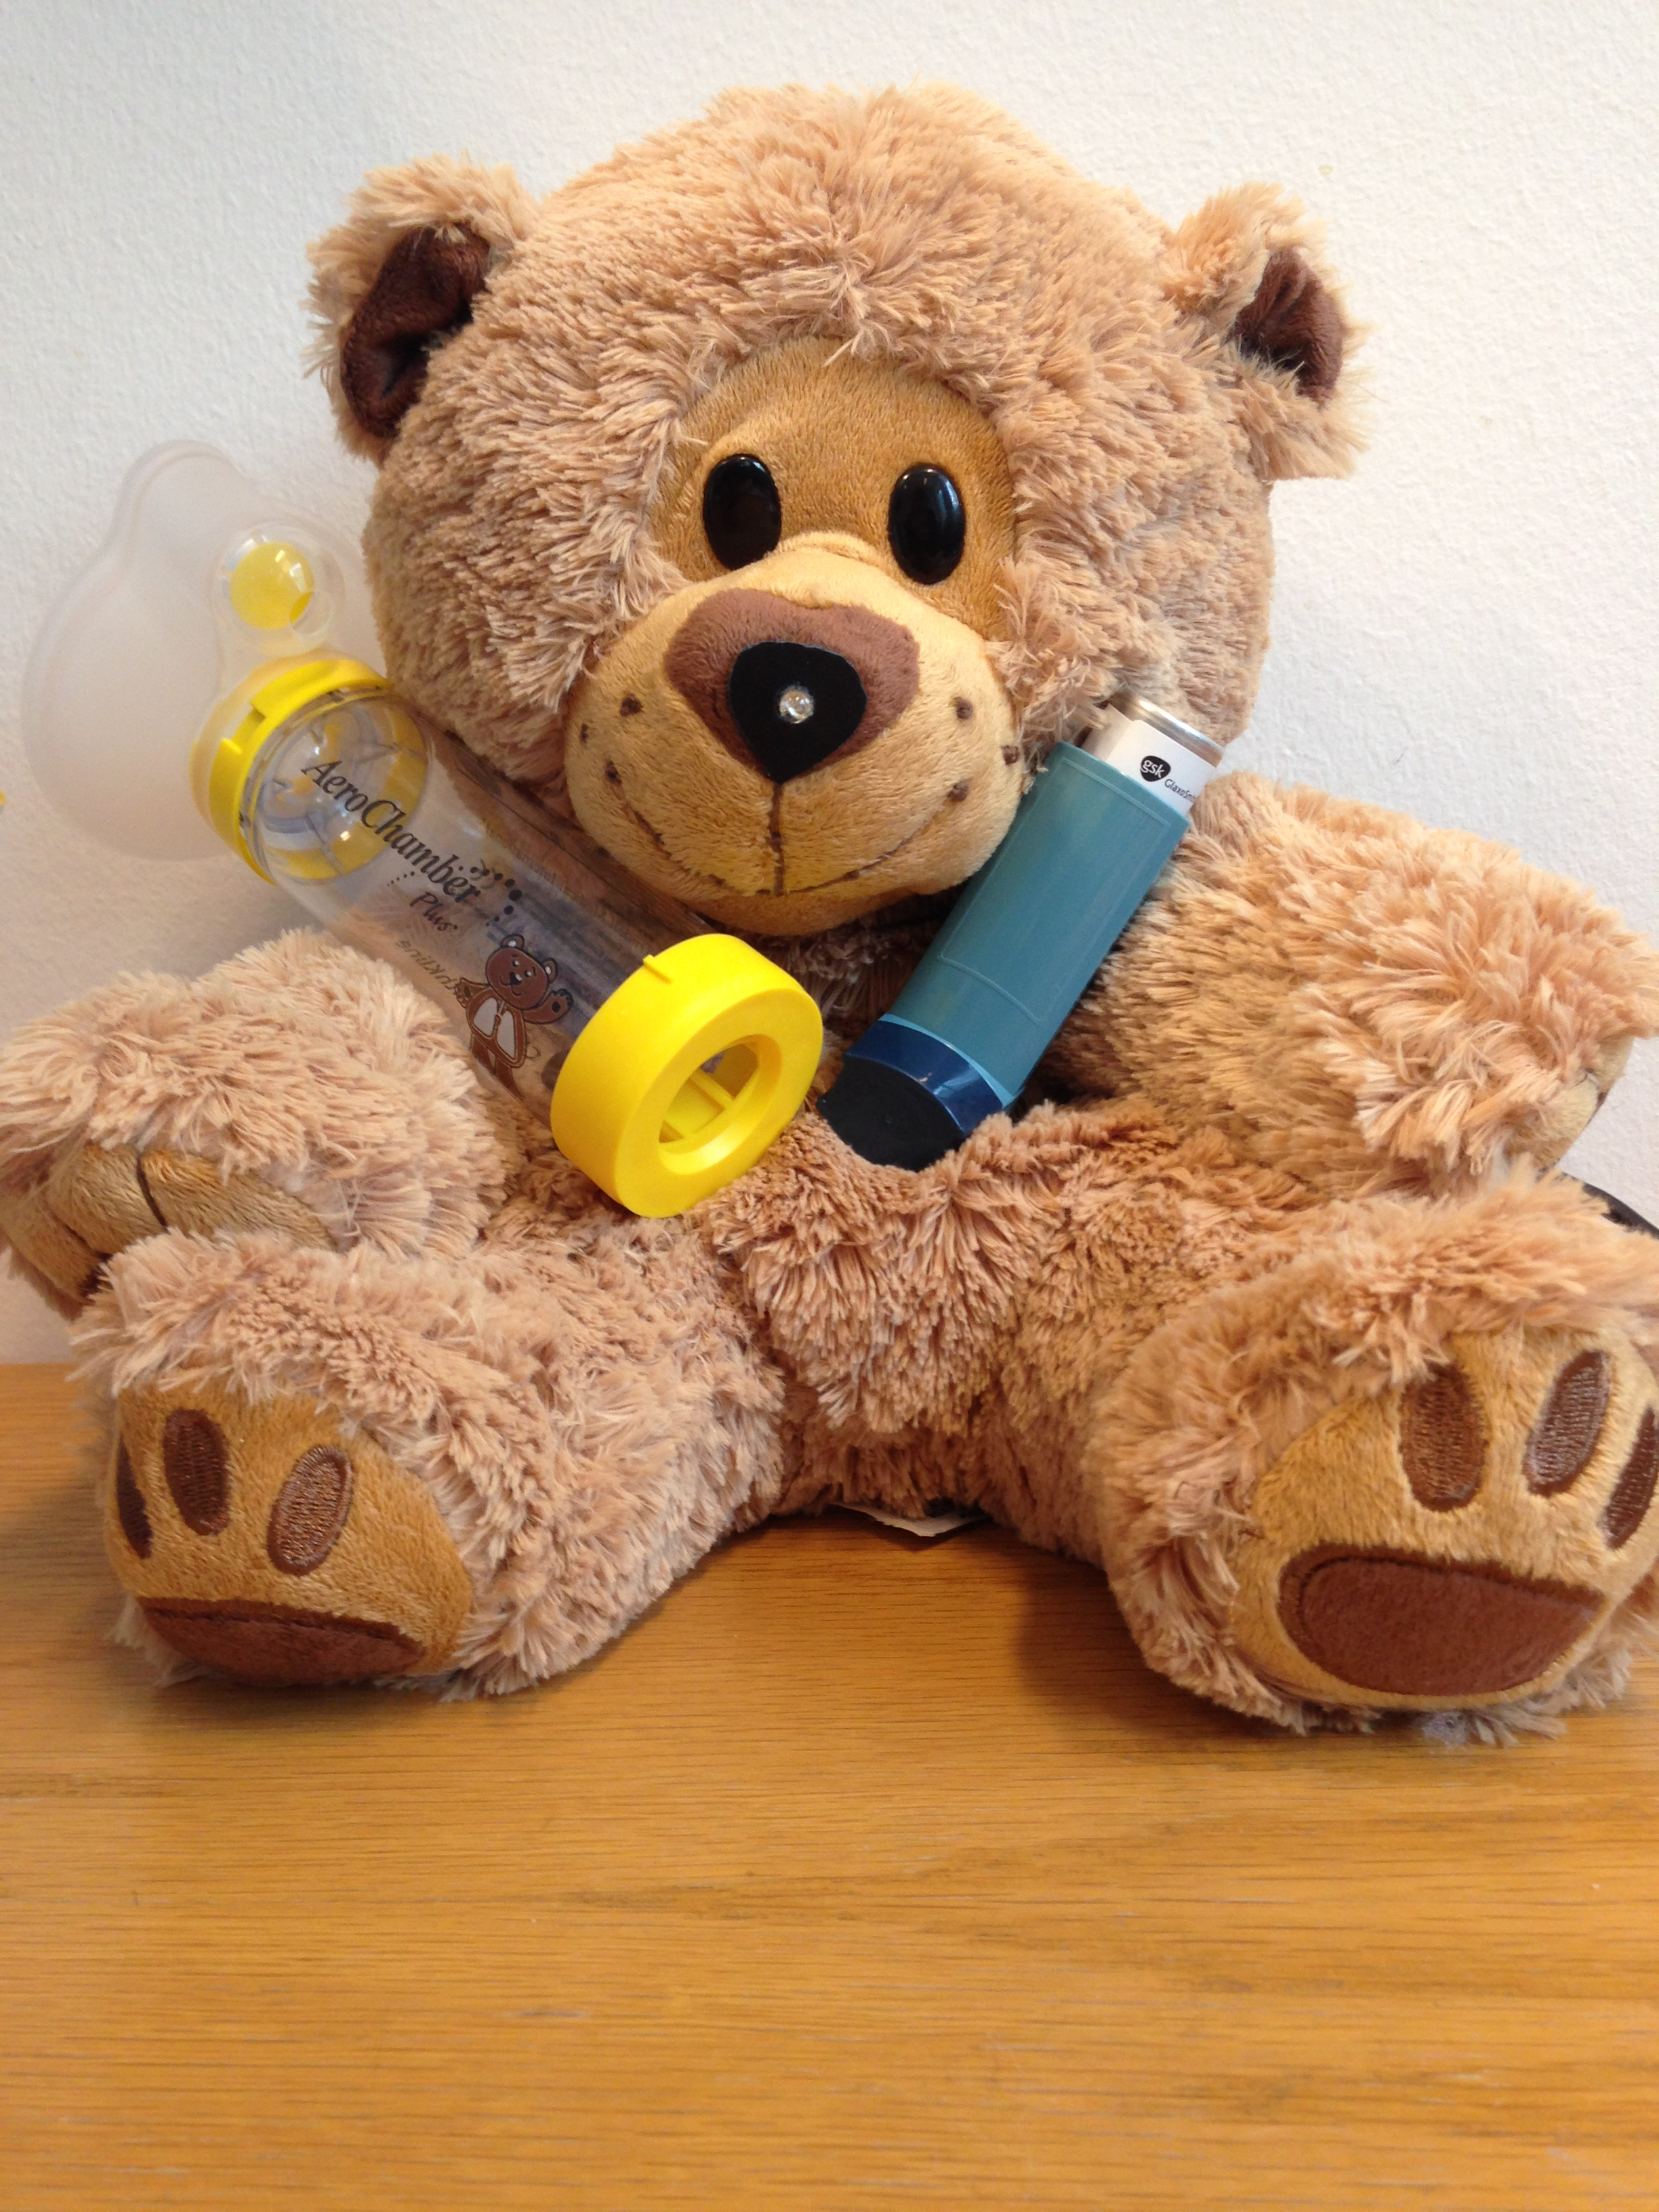
\includegraphics[width=0.3\paperwidth]{Pictures/abandinhaler.jpg}
	\caption[AsthmaBuddy holding a mask and an inhaler]{AsthmaBuddy holding a mask and an inhaler}
	\label{fig:asthmabuddyandinhaler}
	\end{minipage}
	\hspace{2.0cm}
	\begin{minipage}[t]{0.4\linewidth}
		\centering
			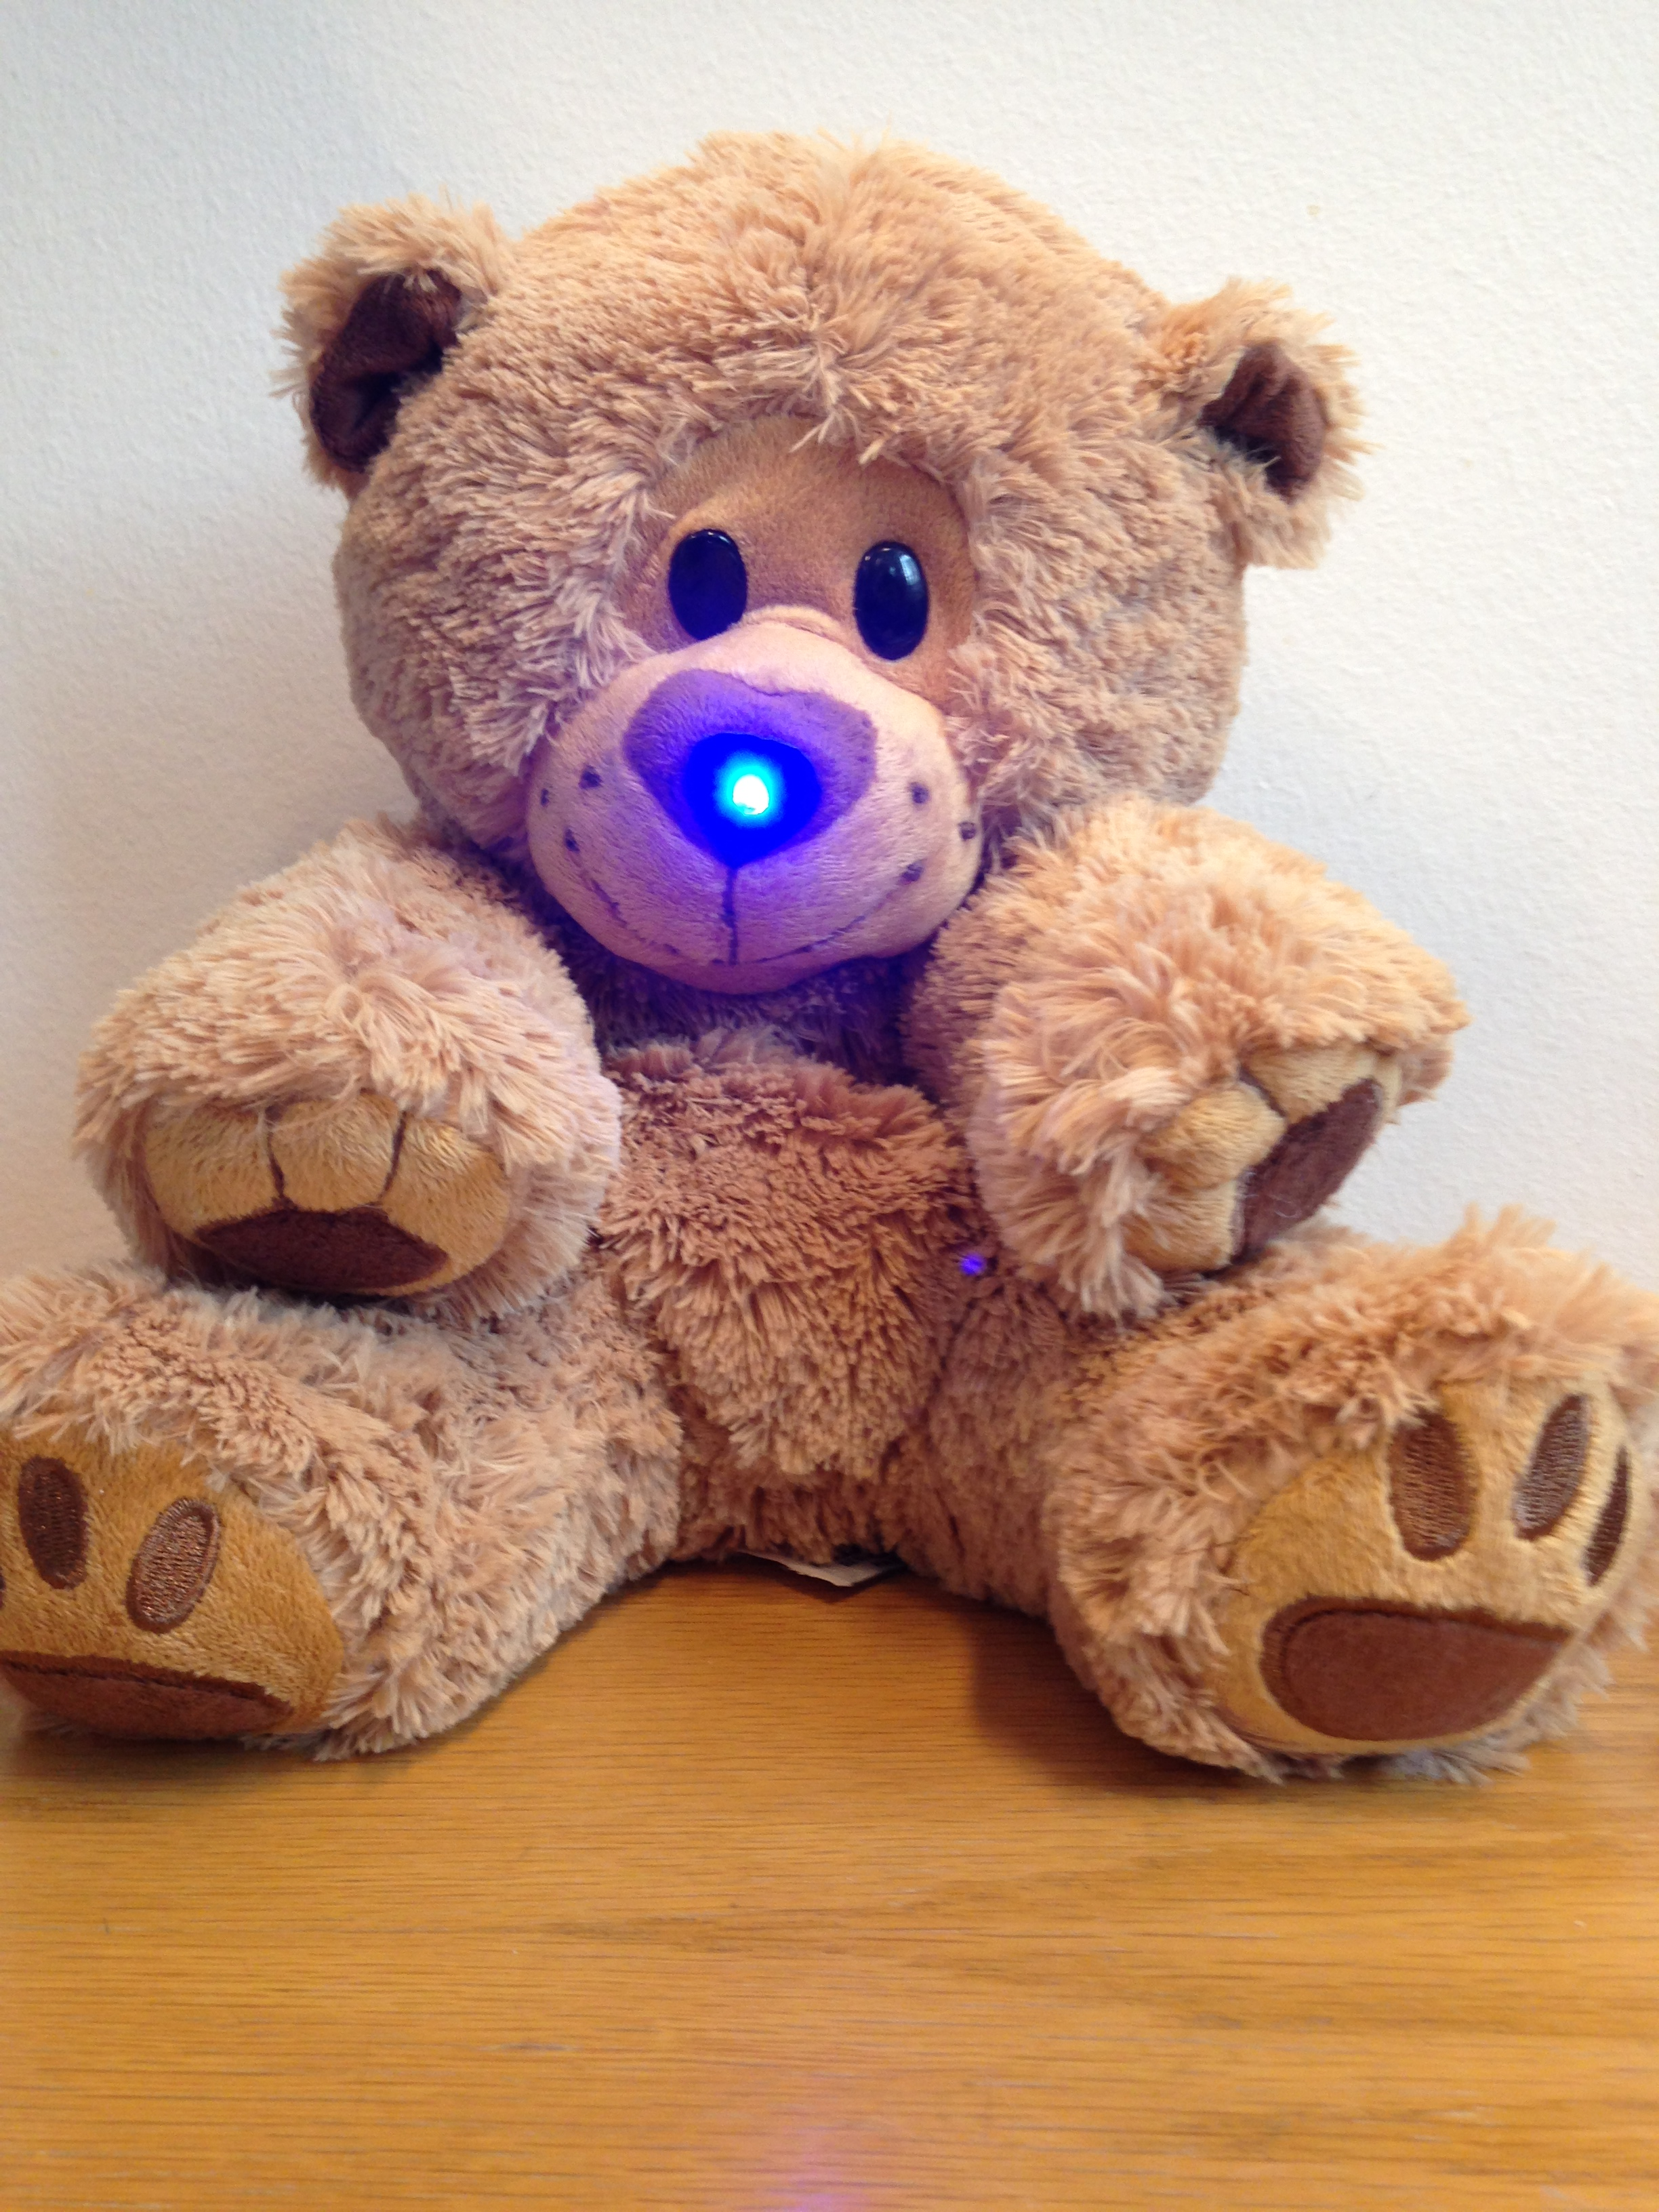
\includegraphics[width=0.3\paperwidth]{Pictures/abbluelight.jpg}
		\caption{AsthmaBuddy with his nose light turned on}
		\label{fig:asthmabuddyandlightnose}
	\end{minipage}
\end{figure}


\subsection{Interaction Design}
\label{sec:interactiondesign}
When we started developing the interaction design of \buddy{}, we had a brainstorming session with the intention of coming up with reasonable interaction patterns.        
By ``reasonable'', we imply that the underlying functionality should be relatively cheap to implement. The interactions should also be fun for the children to perform, in addition to being efficient.  

\begin{table}[H]
	\begin{tabular}{| p{3.0cm} | p{5.5cm} | p{5.5cm} |}
		\hline
		\textbf{Interaction Process} & \textbf{Rationale} & \textbf{Possible implementation} \\
		\hline
		Give \buddy{} a ``High five'' & Demonstrates to children that \buddy{} is friendly. It is intended that a child should keep \buddy{}'s arm up, and high five \buddy{} with the other arm. & A gyroscope and a preassure sensor combined could verify that a high five has been received. \\
		\hline
		Hold \buddy{}'s hand & Demonstrates to children that \buddy{} is friendly. & Preassure sensor within the hand of \buddy{} could solve this. \\
		\hline
		Hold smartphone close to AsthmaBuddy's belly & Could demonstrate the ``smartness'' of \buddy{}, i.e. it can communicate with other things. & Could be solved by Bluetooth. \\
		\hline 
		Press \buddy{}'s nose & Demonstrates to children that \buddy{} is friendly. & Preassure sensor within the nose of \buddy{} could solve this. \\
		\hline
		Press \buddy{}'s belly & Same as above. & Same as above. \\
		\hline
		Hold medicine close to \buddy{}'s mouth & Demonstrates that \buddy{} also needs his medicine. & An RFID-tag attached to the medicine, and an RFID-reader inside the nose of \buddy{} could be used here to control the flow. \\ 
		\hline
		Hold RFID-tag close to \buddy{}'s mouth & Is a relatively easy way to proceed with the process. & A loose RFID-tag could be used together with an integrated RFID-reader, in order to proceed. \\ 
		\hline
		Hold RFID-tag close to \buddy{}'s belly & Same as above. & Same as above. \\
		\hline
		Clap your hands & Should be a fun way of interacting with systems, considering the age of our target group. & Sound recognition could be used here. \\ 
		\hline
	\end{tabular}
	\label{tab:interaction-rationale}
	\caption{Rationale behind \buddy{}'s interaction design}
\end{table}

\subsection{Answering to Champoux's Development Framework}
\label{sec:answeringchampoux}
In Section \ref{sec:champoux} we described the development framework presented by Champoux \etal{} When developing \buddy{}, we tried to answer the proposed questions that we considered relevant. 

\textbf{BO1: What should the user experience?}
The user should experience an interactive guide to applying an asthma treatment correctly. \buddy{} should give correct information in an understandable manner. 


\textbf{BO2: What are the human tasks?}
\begin{itemize}
  \item Fetch an adult
  \item Fetch inhaler and mask
  \item Shake medicine
  \item Attach the inhaler to the mask
  \item Put the mask around your mouth
\end{itemize}

\textbf{BO3: What should the artefact represent and control?}
\buddy{} represents a caregiver, who supervises children during their treatment. The artefact controls that children take their medicine at the correct time, and in a correct manner.   

\textbf{BO4: What are the conventions?}
Children must have their inhaler and mask stored within a short distance of \buddy{}. Their RFID-tags are attached to their inhalers.    

\textbf{OC5a: What is the nature of the interaction for each sub task (Continuous vs Discrete vs Assembly)?}
The subtasks performed when taking a medicine is the following:
\begin{enumerate}
  \item Fetch a grown-up
  \item Fetch inhaler
  \item Fetch mask
  \item Prepare medicine
  	\begin{enumerate}
  	  \item Shake the inhaler
  	  \item Attach inhaler to the mask
  	 \end{enumerate}
  \item Inhale dosage
  	\begin{enumerate}
  	  \item Hold medicine towards mouth
  	  \item Press the inhaler
  	  \item Breathe heavily for 10 seconds
  	 \end{enumerate}
  \item Optional, depending on the medicine: Rinse mouth
\end{enumerate}

Step 4 is an assembly task, 5(c) is a continuous task for a short period of time, while the remaining tasks are all discrete.  

\textbf{OC6: Does the sub-task need any relational interaction?}
None of the sub-tasks needs relational interaction.
[Pieter: Vil RFID-tag og RFID-leser her telle som en form for relational interaction?]
 
\subsection{Dealing with Bellotti's Challenges}
\label{sec:dealingwithbellotti}

Section \ref{sec:challenges-with-TUI} introduced some of the challenges that are encountered when designing tangible interfaces. In the following we will discuss how we handled the challenges encountered, by answering those of Bellotti's questions which we found relevant. 

\textbf{Address: How do I address one of many possible devices?}

One of the challenges mentioned here is ``How to not address the system''. This is an interesting challenge when the system is intended for children, as they are likely to pick things up and carry them around. If a child picks up \ab{}, it could be interpreted as an interaction. We solved this potential problem by only starting treatments in one of two ways, either because it is triggered by an alarm or because an RFID-tag attached to an inhaler is read by \ab{}. The RFID-reader is only capable of reading the tag from a distance of 3 - 5 cm. Thus, as long as no alarm is triggered, and no inhaler with attached RFID-tag is not withing the reach of the RFID-reader, the system should not respond.  


\textbf{Attention: How do I know the system is ready and attending to my actions?}

As mentioned previously, \buddy{} has a LED-light on it's nose. When the light is green, the user can expect that the system is running in idle mode. 

\textbf{Action: How do I effect a meaningful action, control its extent and possibly specify a target or targets for my action?}

The part that regards specifying a target or several targets is considered irrelevant. The interesting part is how the user can effect a meaningful action and control its extent. This will be taken care of by interactions between the user and \buddy{}. \buddy{} will never run several instructions at once. It will always give short and clear instructions, and wait for feedback from the user in order to proceed. 

\textbf{Alignment: How do I know the system is doing the right thing?}

By listening to \buddy{} speak, the user should be aware of what is happening. There is not a lot of room for human error in this connection. By following the normal sequence of operation, the worst thing that may happen is a system crash. This will be handled by shutting down the lights, and \buddy{} will not be running.  

\textbf{Accident: How do I avoid mistakes?}

A part of the challenge is to recover from mistakes that have occured. For instance, if the user proceeds further than what was actually intended, and missed out on an instruction they needed, \buddy{} should have a way to revert to the missed instruction. \ab{} has functionality to replay instructions, but it needs to be told to do so by keyboard input from the ``Wizard-of-Oz''. During user tests, children were told to say ``Repeat'' loud and clear, in order to replay an instruction. Moving beyond the ``Wizard-of-Oz'', this could be handled by a separate form of interaction, eg. shaking \ab{}'s head.       

\section{System Overview}
\label{sec:systemoverview}

\subsection{Use Cases}
Figure \ref{fig:pi-use-cases} shows a general overview of the use cases we have included in our prototype. A medication process can be started set off two ways:
A parent can register an alarm by using AsthmAPP. This alarm is then set of by the \code{AsthmaBuddy} instance running\footnote{The reader should take notice that the tangible user interface \ab{} differs from the program running on the \rpi{}, which is called \code{AsthmaBuddy}(note the change of font)}, giving the child a notification that it is time to take the relevant medicine.

The alternative to a registered alarm is if a child needs to take the medicine by need. In such case, the child or parent simply registers the RFID-tag before the child is guided through a quicker process (see Manuscript \ref{chp:anuscript}).  

\begin{figure}[H] 
	\centering
		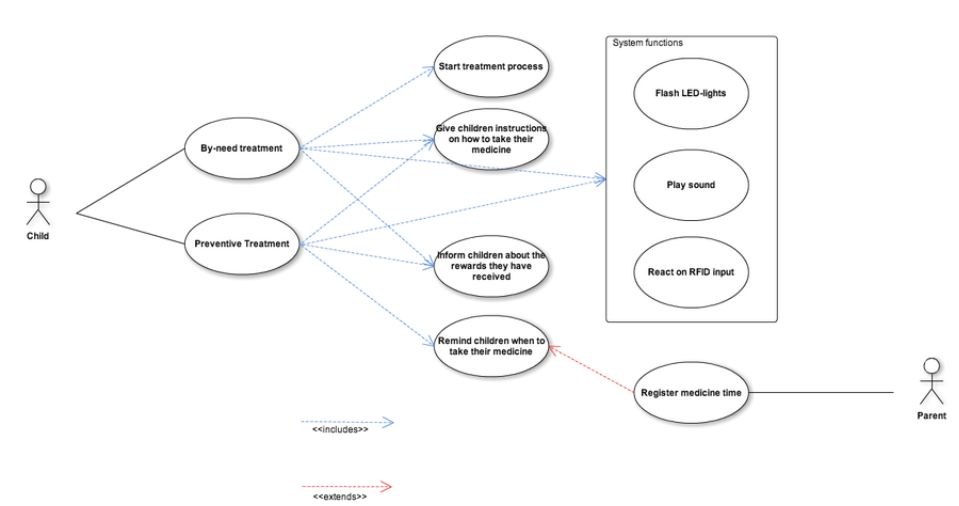
\includegraphics[width=0.8\paperwidth]{Pictures/usecases.png}
	\caption{AsthmaBuddy Use Cases}
	\label{fig:pi-use-cases}
\end{figure}

\subsection{Textual Use Cases}
\label{sec:textualusecasebyneed}

%--------- TEXTUAL USE CASE ----------
%--------- BY NEED TREATMENT ---------
\begin{table}[H]
\centering
\begin{tabular}{|p{4.0cm} | p{9.0cm} |}
\hline
\textbf{Title} & By need treatment \\
\hline
\textbf{Preconditions} & - \\
\hline 
\textbf{Scenario} & 
	\begin{enumerate}
	  \itemsep0em
	  \item User triggers treatment by holding a specific RFID-tag close to AsthmaBuddy.
	  \item System flashes LED-lights to notify user that the system is ready for use.
	  \item System plays sound to instruct the user to shake the medicine.
	  \item System plays sound to instruct user to mount the medicine on the mask and place the mask on his/her face.
	  \item User starts a treatment by interacting with AsthmaBuddy (by pressing it's hand or similar interaction).
	  \item System plays sound to count during treatment (1-2-3-4-5-6-7-8-9-10), while flashing lights for each count.
	  \item System plays sound to tell user he/she has done a good job.
	  \item System calculates reward based on health state.
	  \item System plays sound to award user with the calculated number of stars.
	  \item System plays sound to tell the user how many stars he/she has collected totally.
	\end{enumerate}
\\
\hline
	\textbf{Extensions} & 
		x.a User aborts treatment by not continuing the sequence.
\\
\hline
\end{tabular}
\caption{Textual use case: By need treatment}
\label{tab:textual-use-case}
\end{table}


%--------- PREVENTIVE TREATMENT -------

\begin{table}[H]
\centering
\begin{tabular}{|p{4.0cm} | p{9.0cm} |}
\hline
\textbf{Title} & Planned treatment \\
\hline
\textbf{Preconditions} & The current time corresponds with the time for a planned treatment. \\
\hline 
\textbf{Scenario} & 
	\begin{enumerate}
	  \itemsep0em
	  \item The system recognizes the time for a planned treatment.
	  \item The system starts blinking with LED-lights and playing sound to notify user.
	  \item Child interacts with AsthmaBuddy, to notify that he/she is ready for the treatment.
	  \item Start instructions by playing sound, telling the user to find a grown-up that can keep watch.
	  \item System waits for interaction to make sure the user is ready.
	  \item System tells the user to mount the medicine on the mask and put the medicine towards AsthmaBuddy's face.
	  \item System plays sound to simulate breathing.
	  \item System plays sound to tell the user how easy it was to take medicines and that it is the user's turn.
	  \item System plays sound to instruct user, telling the user to shake the medicine.
	  \item System waits for interaction to make sure the user is ready.
	  \item System plays sound to instruct user to put the mask on his/her face.
	  \item System plays sound counting to 10. 
	  \item System plays sound to tell the user he/she has done a good job.
	  \item System calculates reward based on health state.
	  \item System plays sound to award user with the calculated number of stars.
	  \item System makes a HTTPGet call to the server to find the total number of stars collected.
	  \item System plays sound to inform the user about how many stars the user has collected totally.
	\end{enumerate}
\\
\hline
	\textbf{Extensions} & 
		x.a Child does not interact with AsthmaBuddy when prompted
\\
\hline
\end{tabular}
\caption{Textual use case: By need treatment}
\label{tab:textual-use-case}
\end{table} 


\subsection{State Diagram}
\label{sec:statediagram}

In order to start the AsthmaBuddy application, we used SSH in order to gain access to the computer. We then retrieved the latest version of the source code from Git\fnurl{Git is the Source Code Management system we used}{http://git-scm.com/}, compiled it, and started running it (this process is described in Appendix \ref{app:asthmabuddy_manual}). Once AsthmaBuddy is running, it follows the state diagram depicted in Figure \ref{fig:asthmabuddy_statediagram}.  
  

\begin{figure}[H] 
	\centering
		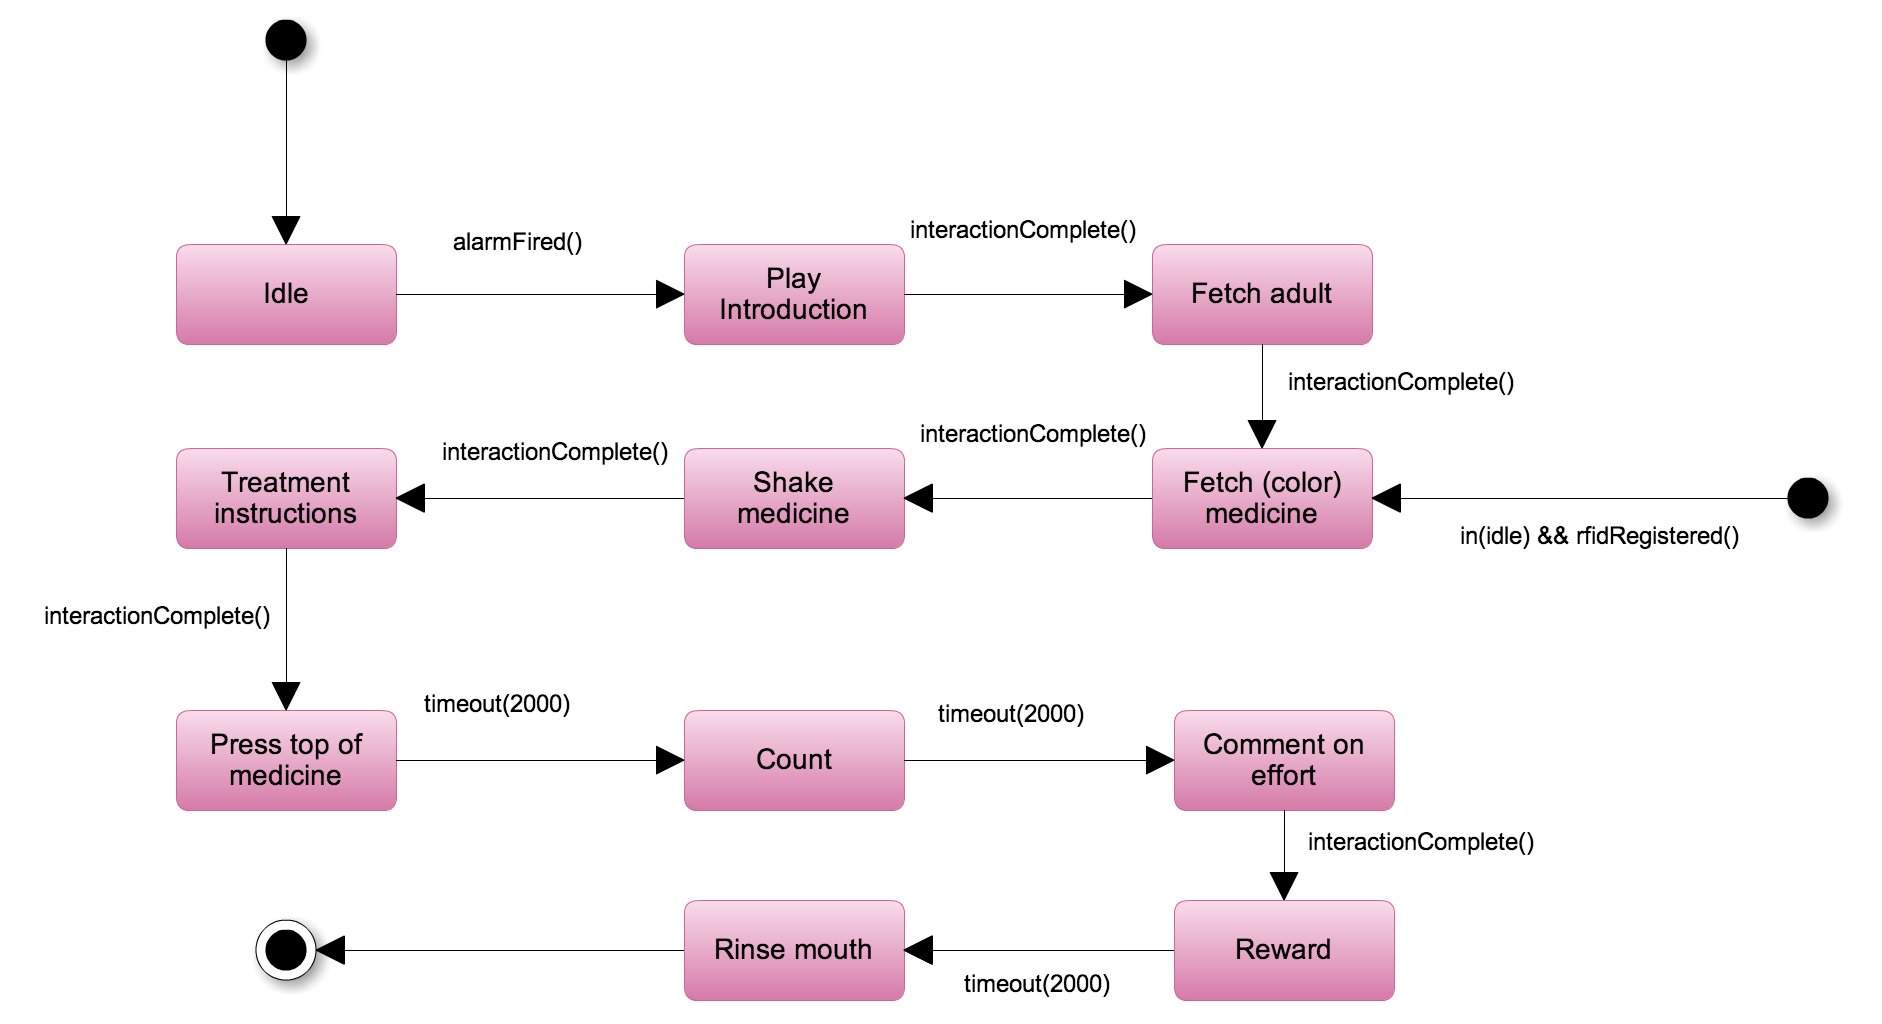
\includegraphics[width=0.7\paperwidth]{Pictures/statediagram.png}
	\caption{AsthmaBuddy State Diagram.}
	\label{fig:asthmabuddy_statediagram}
\end{figure}

\subsection{Sequence Diagram}
Figures \ref{fig:ab-sd-byneed} - \ref{fig:ab-sd-completing-treatment} shows sequence diagrams of how the system works internally. Some abstractions have been made, in order to reduce the cluster of arrows. 

\begin{sidewaysfigure}[htbp]
	\centering
		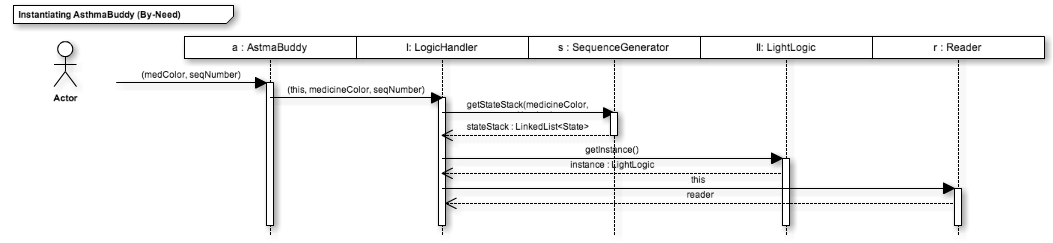
\includegraphics[scale=0.6]{Pictures/sd/sd-byneed.png}
	\caption{By Need Treatment - Sequence Diagram}
	\label{fig:ab-sd-byneed}
\end{sidewaysfigure}

\begin{sidewaysfigure}[htbp]
	\centering
		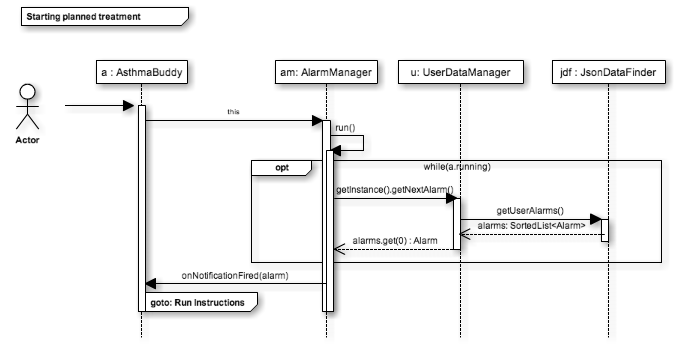
\includegraphics[scale=0.6]{Pictures/sd/sd-planned-treatment.png}
	\caption{Planned Treatment - Sequence Diagram}
	\label{fig:ab-sd-planned-treatment}
\end{sidewaysfigure}

\begin{sidewaysfigure}[htbp]
	\centering
		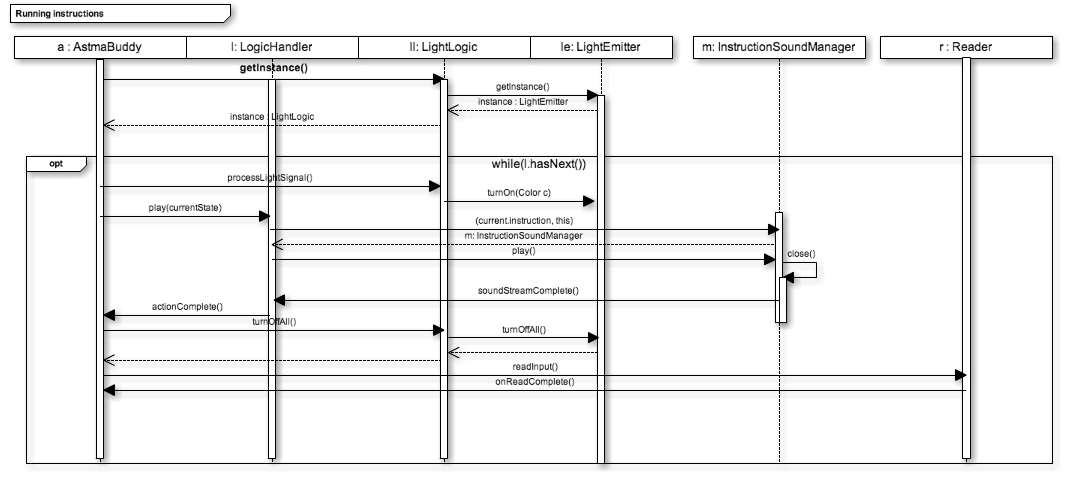
\includegraphics[scale=0.6]{Pictures/sd/sd-instructions.png}
	\caption{Playing Instructions - Sequence Diagram}
	\label{fig:ab-sd-instructions}
\end{sidewaysfigure}

\begin{sidewaysfigure}[htbp]
	\centering
		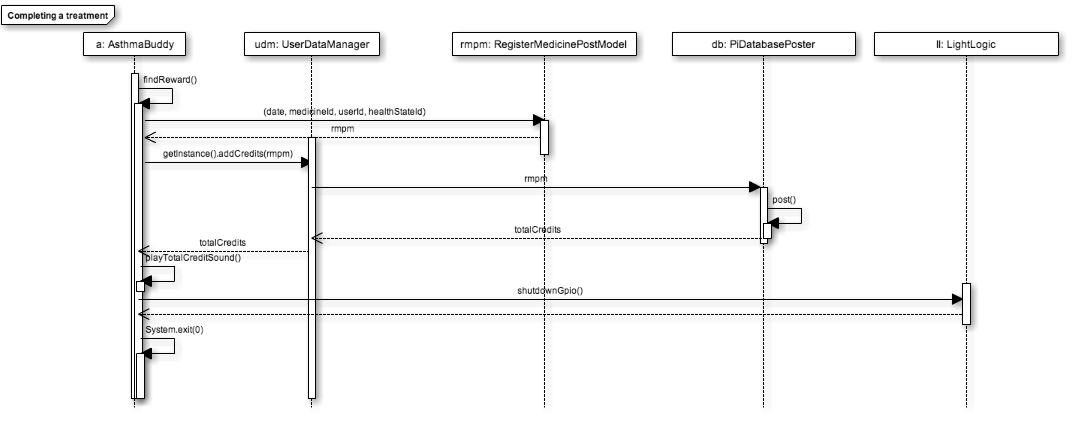
\includegraphics[scale=0.6]{Pictures/sd/sd-complete-treatment.png}
	\caption{Finishing a treatment - Sequence Diagram}
	\label{fig:ab-sd-completing-treatment}
\end{sidewaysfigure}


\begin{sidewaysfigure}[htbp]
	\centering
		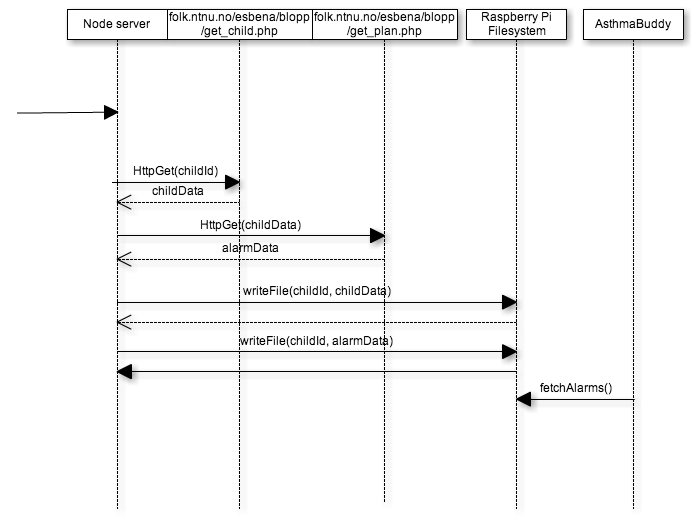
\includegraphics[scale=0.6]{Pictures/sd/sd-synchronizingv2.png}
	\caption{Synchronizing alarms - Sequence Diagram}
	\label{fig:ab-sd-synchronizing}
\end{sidewaysfigure}

\textbf{By Need Treatment}

We were not able to find a reasonable easy way to let the \buddy{} automatically be aware of the medicine that was to be taken at the start of a treatment. As a result, we used ssh into the \rpi{}, and provided the color of the medicine and the sequence number for the interaction that was to be tested.

After inserting these parameters, the \code{LogicHandler} retrieves a \code{LinkedList} of \code{Interaction}-objects that is to be played. After this sequence is ended, the system jumps to Figure \ref{fig:ab-sd-instructions}.
 
\textbf{Planned Treatment}

If an \code{AsthmaBuddy} instance is started without any parameters, it starts looking through alarm files (see Section \ref{sec:node-server}) every 60 seconds. If no alarm is returned from \code{UserDataManager}, it waits. Once an alarm is found, \code{AsthmaBuddy} is notified through \code{onNotificationFired}, which starts the treatment process. 
 
\textbf{Playing Instructions}

Playing instructions is mainly a loop of playing a sound, and turning on and off the LED-lights through the \code{LightEmitter} instance. 

\textbf{Finishing a Treatment}

When a treatment is finished, i.e. we are out of the \code{while} loop in Figure \ref{fig:ab-sd-instructions}, we register the treatment in the database. This ensures that the child is able to see the rewards in AsthmAPP. 


\subsection{Node Server}
\label{sec:node-server}
In addition to the Java application running on the \rpi{}, we developed a Node.js server\fnurl{Node.js}{http://nodejs.org/}. This backend system was developed in order to easily visualize the rewards given to a child after a treatment using \buddy{}. The initial problem is that AsthmAPP stores data to a MySQL database, with \code{childId} as the primary key for most tables. Initially, \buddy{} has no way of knowing which \code{childId} to add rewards to, or for which user alarms should be triggered. The current solution to our problem was to develop a Node.js server on AsthmaBuddy, which run as a background process. Whenever we want to switch users, AsthmAPP does an HTTP POST to this server, including the \code{childId} as a parameter. The server then retrives JSON-formatted data from our webservice, which includes the rewards a child has been given until now (for instance, by using a smartphone), and the alarms set for this user. 
When \buddy{} starts running, it checks for alarms to be set off every 60 seconds. When a child has finished a treatment, \code{AsthmaBuddy} updates the database, with the \code{childId} previously retrieved, and the number of stars a child collected during his/her treatment. With the data retrieved from the database, \buddy{} has the capability to tell the user how many stars a child has collected\footnote{Since this is a prototype, this functionality only works until a child has collected 20 stars. It became cumbersome to handle rewards totalling more than 20 stars}. This process is shown in Figure \ref{fig:ab-sd-synchronizing}.


 

\section{Prototype Version 1}
\label{sec:proto1}

Our first version of \ab{} was supposed to have capabilities to guide a child through a treatment. It was possible to interact with \ab{} through the interactions described in Table \ref{tab:interaction-rationale}. Version 1 did not have the ability to synchronize rewards with \app{}, nor informing the user about the total amount of stars collected. We tested the version on inexperienced users (results can be found in Chapter \ref{chp:interaction-methods}), in order to discover information flaws and difficulties when interacting with \ab{}. We assumed that if an adult was not able to perform a treatment correctly with \ab{}, then children would not be able to do it either.  

We did not have the resources available to implement all of the interaction methods listed. As such, we simulated the interactions through the Wizard-of-Oz technique\cite{wilson1988rapid}.

This version was also used for demonstration purposes during our interviews, which provided us useful feedback on functionality we could add to \ab{}.           
	
\section{Prototype Version 2}
\label{sec:abversion2}
The improved version of \ab{}, hereby referred to as \ab{} 2.0, had some changes done since version 1.0. After testing version 1.0 on inexperienced users, we removed some of the interaction methods. A summary of the interaction methods available in version 2.0 is provided in \ref{chp:interaction-methods}. \ab{} 2.0 is able to synchronize collected stars automatically between \app{} and \ab{}. This was done to automate some tasks that previously needed manual interaction, and to create a tighter coupling between the two prototypes.

\ab{} 2.0 also received some new features, such as a method for letting children more easily check the total amount of stars they have collected. By registering an RFID tag, \ab{} tells how many stars the child has. This was implemented to make \ab{} more of a stand-alone system, and to avoid the problem where parents may not want their child to use their smart phone to use \app{}. 
 
Additionally, some small changes were made to the use of the LED light on \ab{}'s nose. \ab{} 1.0 changed the color of its nose fairly often. This was intended to make the treatment process more interesting; however, it ended up being more confusing than helpful, and was therefore changed to mirror the breaths of the user, and the color of the medicine container. 

\section{Summary}
\label{sec:asthmabuddysummary}
We have developed a prototype for a tangible user interface called \ab{}, who can be used to guide a child through a treatment process. The software behind the prototype is built upon a \rpi{}, which was placed inside \ab{}. We designed a set of interaction methods that we figured could be appropriate for children. This set was narrowed down after a round of user tests on inexperienced users (see Chapter \ref{chp:interaction-methods}). It is currently capable of reading RFID tags, playing sounds and changing the light of its' nose. During the user tests, we simulated the usage of microphones with voice recognition, sensing touches to it's hand, sensing a smartphone's precence and distinguishing between a touch and a high five.       

\chapter{Results}
\label{chp:results}

\section{Interviews}
\label{sec:interviewresults}

We performed interviews on a set of domain experts in order to receive input on the work we had accomplished. Table \ref{tab:interviewsperformed} summarizes the interviews we performed, why we interviewed these subjects and the topics we covered during the interviews. Transcripts from the interviews are included in Appendix \ref{app:interview-transcripts}. 

Where we have interviewed parents of children with asthma, we have named those Parent N (N is a number), in order to protect the identity of their children.  

\begin{sidewaystable}
\centering
\begin{tabular}{| p{3.0cm} | p{4.0cm} | p{3.5cm} | p{6.0cm} | p{2.5cm} |}
	\hline
	\textbf{Name} & \textbf{Background} & \textbf{Rationale} & \textbf{Topics covered (keywords)} & \textbf{Reference to interview transcript} \\
	\hline
	Nanna S\o nnichsen Kayed & PhD/Researcher in Psychology. & Input on reward system. & Rewards for children, Gamification, Motivation. & Appendix \ref{sec:psychinterview} \\
	\hline
	Marikken H\o iseth & PhD cand in industrial design. Experience from the BLOPP project. & Collect data to design for children. & Reward systems for children, designing for children, interaction design. & Appendix \ref{sec:marikkeninterview} \\
	\hline
	Rose Lyngra & Senior Advisor at NAAF. & Has expertise on asthma in general. & Asthma among children, smartphone applications, motivation. & Appendix \ref{sec:roseinterview} \\
	\hline
	Two nurses & Nurses with expertise on asthma treatment. & Collecting data from treatment experts. & Information in \ab{} and \app{}, smartphone applications, problems with asthma. & Appendix \ref{sec:nursesinterview} \\
	\hline
	Parent 1 & Parent of a child with asthma. Has expertise in computer science. & Collecting data from parents. & Asthma in the family, smartphone applications, TUI, motivation, rewarding children, asthmatic child at school/kindergarten. & Appendix \ref{sec:parent1interview} \\
	\hline
	Parent 2 & Parent of a child with asthma. Works in a kindergarten. & Collecting data from parents. & Asthma in the family, reward systems, asthma in the kindergarten, teaching inexperienced users. & Appendix \ref{sec:parent2interview} \\
	\hline     
\end{tabular}
\caption{Interviews performed during the project}
\label{tab:interviewsperformed}
\end{sidewaystable}  

\subsection{Discoveries Found During Interviews}

\textbf{Operating time}

The longest duration for taking a planned treatment was about 2 minutes for an experienced user, and about 2.5 minutes for an inexperienced user. This treatment included the part where \buddy{} completes the treatment before the child. A normal treatment taken without \ab{} usually takes 1 - 2 minutes, according to our interview subjects. Since \ab{} only takes 0.5 - 1.5 minutes longer than normal, it should not be considered a time-waster. From another point-of-view, if a child does not want to take his/her medication, it may cause an argument and it may take a much longer time to complete the treatment. If \ab{} can help on shortening the time spent arguing with the child, a time may be saved.      

\clearpage{}
\textbf{By need treatments}

We got some feedback regarding the \emph{by need} treatments. Some parents stated that they would not use \buddy{} to complete a by need treatment, as their child was suffering from an asthma attack. However, one of the parents noted that if children were used to performing their treatment with \buddy{}, it could create a dependency toward it, i.e. \buddy{} could help the parents to calm the child. Whether or not the by need functionality would actually be used needs more research, as \buddy{} would need to be placed within a home and be nearby when such an attack occurs. 

\textbf{\ab{} as a stand-alone system}

One of the interview subjects commented that \ab{} should be able to operate as a stand-alone system if the parents do not allow the child to borrow a smartphone and the child does not have a smartphone of his/her own. The same interview subject commented that she would not take the time to use \ab{} for two minutes every time the child needed to take a treatment, and that \ab{} might become boring after a period of time.

\section{Testing \ab{} on Inexperienced Users}
\label{chp:interaction-methods}

Before we did user tests on children, we ran a round of tests to verify \ab{}'s ability to explain the treatment process for inexperienced users. We tested on ten students at NTNU, where one of them had asthma during childhood. While doing so, we also tested the different interaction methods \ab{} could be used with. The reason we wanted to test the interaction methods was to get an overview of how adults perceived the interactions. If adult users are incapable of doing some of the interaction methods, we figured that children were probably incapable of doing the same. Additionally, since we had problems to get a significant amount of children to test the system on (which will be elaborated further in Chapter \ref{sec:difficultyfindingtestusers}), we did not want to waste a usability test on a child by initially having a bad interaction design.         

The results of the interaction testing is summarized in table \ref{tab:interactioneval}.  

\begin{table}[H]
\begin{tabular}{|p{4.0cm} | p{7.5cm} | p{2.5cm} |}
\hline 
\textbf{Interaction Method} & \textbf{Comments} & \textbf{Suitable for children?}\\
\hline
	Give AsthmaBuddy a ``High Five'' & Worked out fine. A high five is cool and may make \ab{} seem more friendly to the children. & Yes \\
\hline
	Hold AsthmaBuddy's hand & Easy to understand and use during a treatment. Should give feedback to indicate that the user has interacted correctly. & Yes\\
\hline
	Hold smartphone close to AsthmaBuddy's belly & Smart phones are cool, but may be easily damaged if dropped. To risky to let small children handle a smartphone. The size of the smartphone may require use of two hands, which may cause complications for the child. & No \\
\hline
	Press AsthmaBuddy's nose & Users tended to press the LED light on the nose. Risk of damage to light. & No\\
\hline
	Press \buddy{}'s belly & Easy to understand and use during a treatment. Should give feedback to indicate that the user has interacted correctly. & Yes\\
\hline
	Hold medicine close to AsthmaBuddy's mouth & Created some complications when the user was supposed to hold the mask to his/her mouth and then hold the medicine close to \ab{}'s mouth to proceed. & No \\
\hline
	Hold RFID-chip close to \buddy{}'s nose & The thickness of \buddy{}'s nose made it difficult for the RFID tag to communicate with our reader, this caused problems for the user. & No \\
\hline
	Hold RFID-chip close to \buddy{}'s belly & Works fine. Letting children have their ``magic token'' which interacts with \ab{} may be cool for them. & Yes\\
\hline
	Clap your hands & Works fine. At one point the user has to clap hands when having the mask in his/her hands, which may cause some problems, but should not be a big problem. & Yes\\
\hline
	A variation of the above interactions & Some of the interaction methods made it confusing for the user, e.g. they were asked to hold the medicine towards \ab{} before having fetched the medicine. & Yes, but in a revised form.\\
\hline
\end{tabular}
\caption{Evaluation of interaction methods for AsthmaBuddy}
\label{tab:interactioneval}
\end{table}

\subsection{Observations Made During Tests}

In order for \ab{} to be useful for inexperienced users, it could have even clearer and more informative instructions. Even though it may seem self-explanatory to take the cap off the medicine before mounting it on the mask, it may not be that obvious to new users. Since \ab{}'s purpose is to instruct and inform, it should have a completely ``foolproof'' instructions. For instance some of the test users tried to attach the inhaler to the mask without removing the protective cap from the inhaler. Since the mask's mount is made from rubber, it gave them the idea that one should just push the medicine into the mount by force, which is incorrect. 

When using \ab{}, some users found it difficult to hear all of the instructions. Supporting replay of the last instruction was important. 

\section{Usability Test Results}
\label{sec:usabilityresults}
In order to protect the identity of our test subjects, especially considering the children, we have used identifiers as names. Names starting with the letter ``A'' is an adult user, and names starting with ``C'' denotes a child.

\subsection{Parent partition tests}
\begin{table}[H]
\begin{tabular}{|p{4.0cm} | p{4.0cm} |}
	\hline
	\textbf{Name} & AU1\\
	\hline
	\textbf{Age} & 36 \\
	\hline
	\textbf{Date} & May 2nd, 2014 \\
	\hline
	\textbf{Testleader} & Aleksander\\
	\hline
	\textbf{Observer} & Esben\\
	\hline	
\end{tabular}
\end{table}

\begin{singlespacing}
\begin{table}[H]
\begin{tabular}{| p{1.0cm} | p{4.0cm} | p{4.5cm} | p{4.0cm} |}
\hline
	\textbf{Task} & \textbf{Problem} & \textbf{Cause} & \textbf{Proposal for solution} \\
	\hline
	0 & The user where unable to separate between the image for child and parent partition & The images were not entirely intuitive & The image for adults could have a bearded man, or other recognizable features. \\
	\hline
	1 & It was unclear whether he had to press on the healthy medicine plan, as the child was in the healthy medicine plan by default. & Challenging GUI & Could make it clearer for the user which treatment plan is being followed \\
	\hline
	1 & The spinners for hour/minutes should be able to be written into. & The standard Android slider contains a minor bug when one writes into it.  & N/A \\
	\hline
	1 & The time that shows when the alarm should fire contained seconds, which the test subject found unnecessary. & N/A & Remove seconds from the timestamp \\
	\hline
	2 & The user expected that he could be able to press the medicine, and not just the checkbox which was the case. He found this a little annoying. & Implementation of listener & Make the entire list item touchable \\
	\hline
	2 & He wanted functionality for adding two medicines at once.  & This has not been implemented yet.  & Implement it later \\
	\hline
	3 & The view shows a button with ``Add Activity'', which he felt was wrong. & This was not intended, as it should have said ``Add Reward'' & Change it to ``Add Activity'' \\
	\hline
	3 & The user pressed the back button one too many times. This caused the PIN-challenge to be presented again, which the test user said could be annoying for some users.  & PIN-challenge appears as soon a parent returns from the parent partition. & Could implement a timer who checks when the user last completed the challenge.\\
	\hline
	4 & The test user said it was not logical to see where he could check the air quality cast. & Bad task description & Change task description to make it clear \\
	\hline
	4 & The test user wanted functionality for different views, for instance showing the log for a week or a single day. & Too high expectations & This feature could be implemented with more time and resources.  \\
	\hline
\end{tabular}
\label{tab:test1}
\caption{Usability result}
\end{table}
\end{singlespacing}

\subsection{Children partition}

During the user tests, \ab{} was configured to use the varied interaction scheme. This involved a preset combination of the remaining interactions from Table \ref{tab:interactioneval}. This decision was made in order to test all of the possible interactions, as we did not have enough users to test them one-by-one. 

\subsubsection{Child User 1}
\begin{table}[H]
\begin{tabular}{| p{4.0cm} | p{4.0cm} |}
\hline
 \textbf{Name} & CU1 \\
 \hline
 \textbf{Age} & 6 years old \\
 \hline 
 \textbf{Date} & May 2nd, 2014 \\
 \hline
 \textbf{Testleader} & Aleksander \\
 \hline
 \textbf{Observer} & Esben \\
 \hline
\end{tabular}
\end{table}

\begin{table}[H]
\begin{tabular}{| p{3.0cm} | p{3.0cm} | p{3.0cm} | p{3.0cm} |}
\hline
	\textbf{Task} & \textbf{Problem} & \textbf{Cause} & \textbf{Proposal for solution} \\
	\hline
	2 & It seemed like she had a hard time keeping up with \ab{}'s instructions & The voice of \ab{} was speaking to fast & Record sounds with lower speed \\
	\hline
	4 & It was difficult to drag the medicine above the mask in order to start the treatment & The treatment only starts when the medicine is directly above the mask & Should make this functionality simpler to start.  \\
	\hline
	4 & It was hard for the child to keep ut with the voice of the rabbit. & The voice talked to quickly, and \app{} does not have a repeat functionality when a treatment is running. & Should consider implementing repeat.\\ 
	\hline
	5 & It was hard to get a clean read of the RFID tag. & It was not entirely clear where the user had to put the card in order to get a read. & \ab{} should have an indicator as of where the card should be held in order to be read.  \\
	\hline
\end{tabular}
\label{tab:test2}
\caption{Usability result}
\end{table}

CU1 was very shy when arriving at the test lab. It quickly became clear for us that we had to leave the area and rather observe from the back room, in order for her to speak up. The parent was instructed with the tasks that were to be performed, and he explained the tasks to her. Once we were back stage, she started responding to the instructions given. We made a note that the observer should sit in the back room and observe from there, in order for the children to respond more easily.   

When asked which method CU1 preferred, i.e. \app{} or \ab{}, CU1 replied ``I don't know''. CU1 was also asked if both were equally fun, which to CU1 replied ``Yes''. CU1 was also asked if the usage of \app{} and \ab{} was more fun than a regular treatment, which to CU replied ``Yes''\footnote{There is reason to belive that the answer was biased due to the reward}. We asked if this was because of her reward, which was candy, but we were unable to get a reply. 

\subsubsection{Child User 2}
\begin{table}[H]
\begin{tabular}{| p{3.0cm} | p{3.0cm} | p{3.0cm} | p{3.0cm} |}
\hline
	\textbf{Task} & \textbf{Problem} & \textbf{Cause} & \textbf{Proposal for solution} \\
	\hline
	place & place & place & place \\
	\hline
	place & place & place & place \\
	\hline
	place & place & place & place \\
	\hline
	place & place & place & place \\
	\hline
	
\end{tabular}
\label{tab:test1}
\caption{Usability result}
\end{table}

\begin{table}[H]
\begin{tabular}{| p{3.0cm} | p{3.0cm} | p{3.0cm} | p{3.0cm} |}
\hline
	\textbf{Task} & \textbf{Problem} & \textbf{Cause} & \textbf{Proposal for solution} \\
	\hline
	place & place & place & place \\
	\hline
	place & place & place & place \\
	\hline
	place & place & place & place \\
	\hline
	place & place & place & place \\
	\hline
\end{tabular}
\label{tab:test1}
\caption{Usability result}
\end{table}



\section{Evaluation}
\subsection{\ab{}}

After completing all of the validation tests, it occured to us that not one out of the three children we tested \ab{} with were able to listen to \emph{every} instruction and interact accordingly. I.e. every user had to make use of the repeat functionality. There is reason to believe that this is a problem caused by the speed \ab{} talks in. It seemed like a somewhat hard task for children to keep up with both the instruction, e.g. ``Shake the blue medicine, and fetch it to your mask'', and the interaction that was to performed, e.g. ``Clap your hands to proceed''. 

As mentioned, CU3 discovered that \ab{} was not stable enough to handle a proper high five. This problem would probably have been avoided if the child had gotten used to interacting with \ab{}, giving him more knowledge of which preventive measures that needs to be taken, e.g. supporting his back while giving him the high five. However, a more valid argument is that the choice we made regarding \ab{} as a teddy bear was not ideal in the first place.  

Overall, it seemed like all of the children were able to interact with \ab{} as intended. Additionally, it seemed like all of the children found \ab{} enjoyable. 

\subsection{\app{}}

During the user test on AU2, we discovered a critical error that almost rendered the application completely useless. The error originates from the fact that \app{} needs to communicate with the database, and we had not implemented proper feedback to the user that an error had occured. This error should obviously not have occured in the first place, as these types of errors will result in less incentive for parents to use \app{}. 

As for the children, it seemed like all of them liked to use \app{}. However, with the low sample size and the fact that it was children we tested in mind, it is reason to question the validity of this result. On one hand, none of the children had big problems to do what \app{} told them to do and had very few problems navigating the application. On the other hand, the only child capable of reading was CU2, who is seven years old. It should have been given more of an effort to make the process of purchasing a reward even more clear for the youngest users of our target group.     

As far as the gamification system goes, it seemed like children were happy with the fact that stars appear immediately after the treatment is finished. They also seemed happy with the rewards they were given. However, a question that remains unanswered is whether our approach to a gamification system is sustainable over a longer period of time. 

% Critical errors that should have been avoided. 
% Instructions were Understandable for children
% Easy interactions
% Positivt at stjerner kommer med en gang.
% Repeat burde blitt implementert. 
% Flere konkurrenter paa markedet.  

\chapter{Evaluation}
\label{chp:evaluation}

As with all other software development projects, the development of AsthmAPP and AsthmaBuddy has hit some bumps in the road. This chapter will look into possible improvements of the developments process. Second it will evaluate the experiment design and point out different elements which could have been done differently.
 
\chapter{Discussion and Conclusions}
\label{chp:masterconclusion}

This chapter completes the discussion chapter by representing the research questions, providing answers where possible, and evaluates the process of obtaining these answers. 

\section{Discussion}
\label{sec:discussion}


\subsection{Gamification}
\label{sec:gamificationresults}

\subsubsection{Understanding Children's Perception of Rewards}
\label{sec:understandingchildrensperceptionofrewards}

Our proposal for gamification elements contained within \app{} is tightly coupled with the parents' initiative. In order for our reward system to have any motivational effect, parents have to be closely involved. They need to understand how often their child needs a reward, in addition to understanding what defines a ``good'' reward for their children. 

Webster-Stratton and Herbert claims:

\textit{``Preschool children aged between the ages of three and four may be rewarded by the special sticker or token itself without needing a back-up reinforcer. Youngsters aged four to six should be able to trade in stickers for something each day if they like. Children of seven and eight can wait a few days before getting a reward.''}\cite{webster1994troubled}

In order for our systems to have a motivational effect, parents have to be aware of their children's maturity. Rewards that suit a three year old girl do not necessarily suit a six year old boy. Webster-Stratton further claims that parents should expand the efforts children have to put into a task, in order to receive their reward. We will elaborate more on this in Section \ref{sec:gamificationovertime}. 

Parents could be under the impression that the rewards given should be something material. However, according to Nanna S. Kayed, researcher/PhD in psychology: 

\textit{``Rewards do not have to be a material reward, it may be a fun activity or letting the children choose what they will eat for dinner. Doing something entertaining with their parents can be as much of a reward as a physical toy. An example of an easy and fun reward is to eat dinner underneath the table or taking a walk in the woods. It is important for you [the developers] to tell the parents that the reward does not need to be material, but can be simple and easy rewards.''}

She implies that spending quality time with the family can in fact be just as effective as material rewards. She also pointed out that we should include some sort of manual to our reward system, in order to maintain the maximum motivational effect and ensure that parents understand that the rewards do not have to be material. However, creating a manual for reward systems for children could be an own master thesis in psychology, and we will not delve further into this aspect. 

It is reasonable to assume that most parents have used some sort of reward system with their child, for instance to get their child to behave the way the parents want them to. One of our interview subjects had used stickers in order to toilet-train her son. The amount of rewards and their ``attractiveness'' should be correlated to the task performed by the child.

\textbf{``Collectors'' vs. ``spenders''}

Children perceive rewards in a different manner. Some children like to collect their rewards and will never choose to spend the rewards as a currency. To these children the collected amount of rewards is important, and they often value the rewards more as a collector's item than as a currency. 
Some children like to spend their rewards and cash them in as currency. These children often care more about spending the rewards on items rather than saving the rewards, even if the item they spend their reward on is a short-lasting joy, such as an edible item or an arcade credit.
\app{}'s reward system is made to accomodate the wishes of both ``collectors'' and ``spenders''. Since the reward system is a milestone-based system where the stars do not disappear when a reward is purchased, both user types may have what they want. Making the reward system as motivating as possible will be up to the parents.

\textbf{Understanding the family situation}

It may be argued that our reward system could cause internal jealousy within a family. For instance, if a family has three children, where two of them suffers from asthma, the last child could potentially become jealous of the other two, as they may receive rewards which seems unfair for the last child. In such cases, we leave the responsibility to the parents to balance these rewards, such that it does not seem unfair for the healthy children in their family.    

\subsubsection{Bartle's Four Player Types}
\label{sec:bartlesfourplayertypes}
In Chapter \ref{sec:bartlesplayertypes} we presented Bartle's four player types and how they enjoy gamification. In order to understand how gamification can be used in order to motivate children with asthma, we have explored some solutions for how to build an enjoyable gamification system for the four player types; achievers, explorers, killers and socializers. 

\textbf{Killers}

In Chapter \ref{sec:killers} we stated that hopefully no children in our target group hope to gamify their experience by imposing themselves on others. We found no positive and meaningful way to support ``killers'' in our system. The only scenario we could come up with was that children could slow down the progress for others (e.g. steal other children's stars), which is against the purpose of \app{}.  

\textbf{Socializers}

While AsthmAPP has little support for socializers, we believe there is potential for use of social features in a system such as AsthmAPP. An example of such would be the use of an avatar system where the children may share their avatar with others and meet other users of AsthmAPP in a social hub similar to Club Penguin\fnurl{Club Penguin}{www.clubpenguin.com} or Farmville\fnurl{Farmville}{www.farmville.com}. 


\textbf{Explorers}

AsthmAPP in its current state has little to explore. However, we believe that there is a potential for functionality to motivate explorers. The use of progress bars, leveling systems or achievements and badges can easily be transferred to a system like AsthmAPP in order to achieve a gamified experience targeted at explorers. Linander's interactive story concept showed how the progress in a story may be tied to the use of asthma medicine\cite{linander2013utvikling}. Possibilities for adding new stories over time would create an even more engaging system for children. 

\textbf{Achievers}

AsthmAPP mainly provides game elements suitable for achievers. The gamification system in \app{} is built around performing a treatment correctly and being rewarded for doing so. The use of stars as experience points and support for real-world rewards through the shop is applicable for all children, but may be of most interest to achievers. There is endless potential for how gamification may be used to engage achievers, and there are many possibilities for further research on these areas. 


\subsubsection{Reception of AsthmAPP's Reward System}
\label{sec:receptionofrewardsystem}
In order to get feedback on the gamification system of \app{}, we asked our test users and interviewees what they thought about our solution for gamification. Specifically regarding how the reward system racks up when the user is following the yellow and red treatment plan, we received interesting feedback.

\emph{``I think that there should be no differentiation in the rewards at all. One star per treatment should do, regardless if the child is in good or bad shape. In general a sick child would need to take more [typically blue] medicine anyway, resulting in more stars. If there is a multiplication factor in addition to the increased number of treatments the number of starts would go up quite quickly and from the psychological perspective it might make the child think it is a good thing to be ill.''}

This statement differs to an argument made by one of our other interview subjects:

\emph{``It is difficult to determine if there is a risk of children pretending to be sick. Children often do not like going to the doctor's office, which may stop them from pretending to be sick.''}

Due to the contradictory arguments, we are not in a position to make an assessment on how the stars should be awarded, and we advice further research on how the different treatment schemes should be linked to the amount of stars received for completing a treatment. 

\subsubsection{Gamification over time}
\label{sec:gamificationovertime}
According to Webster-Stratton and Herbert, parents have a tendency to not phase out reward systems\cite{webster1994troubled}. When this occurs, children do not receive the message that is in the essence of reward systems; that parents expect their child to perform a task on their own without receiving a reward. In the example Webster-Stratton \etal{} describe regarding raising a child, parents could give a reward for making the bed every day for one week. After a week, the parents should expand the task to include making his/her own breakfast every morning. Similarily, parents should increase the cost for receiving a reward in \app{}.  

Based on findings we did during Customer Driven Project\cite{CustomerDriven}, we believe that gaining access to a new star could be rewarding enough when a child first starts using AsthmAPP. After a while, it will become boring, and parents should provide a means of a tangible reward (material or social). For instance, parents could start out by giving an ice cream sandwich to their child if they take his/her medicine as planned during the first day. Then they could expand the challenge by one day, giving the child some extra allowance if they manage to do it two days in a row. When time passes and their child has gotten used to taking the medicine, the system should be phased out. \app{} in its current state would then serve the purpose of reminding, informing and logging the user's use of medicine.

\subsubsection{The use of different gamification mechanics}
\label{sec:gamificationinthefuture}
When building \app{} and \ab{} we chose to focus on the use of real-world rewards, mirroring user behaviour and experience points. While these were the elements we chose, there are endless possibilities for other combinations of game elements. In the following, we discuss the potential use of different game mechanics in the future.

\textbf{Avatar systems}

The use of avatar systems has huge potential for gamifying the treatment for children suffering from asthma. An avatar system can be a simple game where the user is rewarded with clothing and equipment for their avatar, or too a extensive game where the users use of asthma medicine controls an avatar in a game. Linander's ``Concept for Improved Experience of the Treatment of Asthma''\cite{linander2013utvikling} showed potential for this.

\textbf{Achievements and badges}

There are many possibilities for the use of achievements and badges. Examples of this is badges for ``Follow treatment plan for 5 consecutive days'' or ``''. The use of achievements are two-edged sword. They must not be of a manner that may lead to a non-positive behaviour, i.e. ``Not have an asthma attack for one week'' where the user may not want to use Ventoline, in order to win an achievement. 

\textbf{Real-world rewards}

Our application is built around real-world rewards. We believe there are many possibilities for the use of real-world rewards when it comes to treating children with asthma. We also believe that having real-world rewards will motivate the children over time, since a candy bar, a trip to the local lake or a ticket to the local football match will not wither over time. 
Real-world rewards demands more from the users, since it demands that a parent or an adult gives the child the rewards. While this might help motivate the children it may also put too much work on the parents, and they may see the reward system as too demanding.

\textbf{Mirroring user behaviour}

Mirroring user behaviour has recieved positive results from younger users, and there have been an increased amount of applications using this gamification technique. Applications such as the Grush toothbrush\fnurl{Grush}{https://www.indiegogo.com/projects/grush-the-gaming-toothbrush-for-kids\# home} is built around mirroring user behaviour. 
We find user behaviour a positive and useful technique.

\textbf{Leaderboards}

We had trouble finding how to implement leaderboards in an ethical and positive manner. Using a leaderboard risk breaking Norwegian privacy laws, which is unacceptable. Making the use of medicines into a competition would probably recieve heavy critique, since it may be viewed as a move to increase the income of the companies manufacturing medicine. While the use of anonymous avatars and usernames may combat the privacy concerns, it may still be viewed as unethical and a bad marketing scheme.  

\textbf{Social networking}

One should be very careful when designing social networks for people who suffer from a disease. There are many privacy concerns to take into account. An anonymous social network may be positive for parents with asthma. They may share success stories, ask questions and recieve help through the network. 

\textbf{Progress bar}

There are possibilities for the use of a progress bar within an application for health care. While it will be impossible to evaluate the progress towards being cured from a disease, there are other uses. Combining a progress bar with experience points is easy to implement and have many possibilities for how developer wants to make use of the gamification element. 

\textbf{Experience points}

As mentioned previously, experience points there are many possibilities for the use of experience points. The main challenge with using experience points is to make them have a meaningful value over time. As McGonigal argues, gamification withers over time and there is risk for boring the user\cite{jane2011reality}.  

\textbf{Contests}

As with leaderboards, making the use of medicines has it's risks. One might think of contests such as ``remember to follow treatment plan perfectly for a long period of time'' as a suitable contest, since it has a positive competition. However, this will be in conflict with Norwegian privacy laws. 

\subsection{Tangible User Interfaces}
\label{sec:resultstui}
During our project we discovered different areas where tangible user interfaces may be of use for asthmatic children, their parents and other caregivers. The main areas include learning, motivating, distracting and informing. Other areas where TUIs could be of use are elaborated on in Section \ref{sec:otheraspects}.


\subsubsection{TUI as a Tool for Learning}
\label{sec:tuiasatoolforlearning}

When a child gets diagnosed with asthma, his/her parents receive a lot of information at the doctors. It occurs that the parents are not paying attention, do not understand the information received, or do not communicate the information correctly to other caregivers. As two asthma nurses stated in an interview: 

\textit{``We always make sure to teach the parents and the children how to apply the medication correctly, however, they may forget it over time. If the parents do not remember how and when to give the children medications, it may have a negative effect on the treatment of the child's asthma.''}

\buddy{} can be used to relieve parents from the responsibility of remembering exactly how and when the medicine should be taken. Parents will probably remember the process after a couple of days, but \buddy{} could help them get started. 

Hospitals hand out flyers and treatment schemes to parents when children are diagnosed with asthma. However, flyers are often lost, and miscommunication often occurs when parents leave their child with other caregivers, like grandparents, babysitter, etc. By sending the child off together with \buddy{}, the implications of any miscommunication could be minimized.    

\textbf{Teaching children}

In addition to teaching parents about asthma, \buddy{} could be used to teach children about their disease. In some cases, parents do not explain to their children why they are sick, and what is causing their breathing problems. After a child has taken a dosage, \buddy{} could proceed to read a book about asthma, specifically written for children. As more treatments have gone by, new chapters can be read, increasing children's knowledge and awareness of their disease.   

\textbf{Information correctness}

When informing children and parents about asthma, it is vital that they receive correct information. If the information provided contains errors, it could have significant consequences for the asthma treatment. The information provided should be approved by either medical doctors or organizations like NAAF. This will provide a quality assurance, in addition to gaining potential families' trust.    

\textbf{Understanding their disease}

One of the nurses we interviewed, stated the following: 

\textit{``Children below your target group (i.e. younger than 3 years old) can be even harder to motivate, as children in the group 3 - 5 years old have an understanding as to why they need to take their medicine.''}

Children in the age of 3 - 5 years old understand that they get better from taking their medicine. However, not all parents tell their child specifically what is wrong with them. One of the interview subjects noted that mistakes do occur, and some parents do not understand all of the information received while at the doctor's office, which can result in parents communicating wrong information to their children. 
 
\buddy{} could have been used to inform children about what happens with their lungs before and after they take their medicine.
Some children may get a better understanding of their disease and therefore understand better why they need to remember their medication. There is always a risk that children will be scared when told what their asthma is doing to their lungs. The parents must be aware of how worrisome their child is. 



\subsubsection{TUI as a Tool for Motivating}
\label{sec:tuiasatoolformotivating}

\textbf{Feedback}

Tangible user interfaces could be used to give feedback to children about their treatment. They could for instance notify how good they have been at taking their medicine during a week, and notify if they have forgotten a medicine at a day. This feedback should however be discrete and implemented in a non-obtrusive manner, as parents could interpret \ab{} as yet another annoying toy in the house.   


\textbf{Calming children down before a treatment}

If children are scared before they take their medicine, tangible user interfaces could help calming children down. A friendly character such as a teddy bear might help distract the children from the situation and make them forget about what scared them in the first place. 


\textbf{Turn the process into a game}

TUIs could be used to motivate children by turning each treatment into a game. At the moment, \ab{} and \app{} makes the long run process into a game. A TUI could be used to turn a single treatment into a game, e.g. by saying that \textit{``If you take the cap off the medicine, you get ten points''} and \textit{``If you breathe for ten seconds, you get a hundred points''}. Then children could do the math to calculate their total sum, that the TUI can state is correct or incorrect. 


\textbf{Responsibility}

A TUI could be used to make children more responsible regarding their own disease. Children could for instance be prompted to check whether there is enough medicine in their inhaler, and be responsible for telling their parents if they need new supply. \ab{} could be used for the same purpose by waiting to trigger an alarm, and check to see if the child reacts upon this. If the child reacts, it could provide positive feedback, and if the child does not react, it could give a strict notice that they can't rely entirely on a stuffed toy animal\footnote{This could prove to have a negative effect, but is an option to give children more responsibility.}.  
%TODO: Should we write this somewhere
%Children often become dependent on certain artefacts to accomplish a task. For instance, some children are not able to go to sleep without their favorite stuffed animal. A similar dependency could occur when taking their medicine with \ab{}. 

\subsubsection{TUI as a Tool for Distracting}
\label{sec:tuiasatoolfordistracting}

\textbf{Distracting children while taking a medicine}
In its current state, \ab{} distracts children while taking their medicine by counting to 10, which is the number of seconds a child should breathe in his/her breathing chamber. Additionally, the LED-light at its nose is blinking, which we will discuss further in Section \ref{sec:dosanddontsfortui}. 

Since we only have 10 seconds to work with, there are big limitations on what \ab{} can actually do in order to distract them in a natural way. It could be argued that having \ab{} by their side is actually enough distraction, as they have something to look on. If a TUI with movable parts had been developed, these parts could be used to give children something else to look on, by for instance introducing them to a new dance once in while.        

A more interesting case would be to distract children that are using a nebulizer in their treatment, as these often lasts for about 10 minutes or more. Children would then have to rely on something more exciting, like an audio book. 

\textbf{Distracting children between medicines}

Children often have to take two different medicines after eachother, but not immediately. A reguler scheme is to first take Ventoline, then wait for five minutes, before a dosage of Flutide should be taken. One of the interview subjects pointed out that: 

\textit{``The teddybear could help children to keep up with the time while they're waiting to for the next dosage.''}

He further noted that it was easy to get ``overly excited'' and take the Flutide dosage earlier than 5 minutes after Ventoline has been taken, which will reduce the effect of Ventoline. \ab{} could in this case distract the child from taking the medicine too early, by for instance reading an audio book, playing songs or even count down to the next dosage. The effect this distraction could vary from child to child. If a child really hates to take his/her medicine, having \ab{} count down to the next dosage could seem frightening for the child.   
  

\subsubsection{TUI as a Tool for Informing}
\label{sec:tuiasatoolforinforming}
For children with astma there is a lot to remember. We have already discussed the theme of learning about asthma, which is a very important aspect. There is still more to remember, and we have found some ideas for what the tangible user interface may help for. 

\textbf{Counting doses left in the inhaler}

One of parents we interviewed noted that: 

\textit{``It is annoying when medicines go empty, so we're keeping a journal''}

Since the inhalers have a certain amount of doses in them, and the amount of doses varies between different medicines and their vendors, it may require an effort to remember how many doses are left. The disk-formed medicine often come with an indicator, while inhalers do not. Inhalers make a ``poof'' sound when pressed, and this sound may occur regardless of whether or not there are any doses left. By using a RFID on the medicine and a RFID-reader on the TUI, may keep up with how many doses have been taken, and the system automatically warns the user when the number of doses is running low. There are many other ways to solve this digitally, but we believe that having \buddy{} count how many doses are left and  tell the user by sound could be fun for children and helpful for parents.


\textbf{Pollution levels and pollen forecast}

There are many different applications and web pages for reading and recieving information about air quality and pollen forecast. These web sites often offer data to third party services. AsthmAPP has the functionality for getting air quality readings and pollen forecast in the same application (see Chapter \ref{sec:description-medicine-log}).
\buddy{} could help the children with the same functionality, starting the day by telling how the air quality and pollen readings are for the day. 

In a future version, \buddy{} could calculate and foresee the amount of medicine needed when there is much pollen or bad air quality and update its alarm schedule based on the knowledge gathered. However, this is a functionality which will require further research.


\textbf{Reminders}

\buddy{} has functionality for firing alarms based on the treatment plan set in AsthmAPP. This makes it easier for the children and parents to remember to apply the treatment at the planned time. While taking medicine is often a routine for families with asthmatic children, \buddy{} could be a useful embodyment of a reminder. 

In a future version \buddy{} should be able to know that if a treatment has been completed within a short time before a planned treatment, the planned treatment will not be necessary. For a user having completed their planned treatment, an alarm firing 5 minutes later can be annoying. \buddy{}'s purpose is to help the user to remember, and if the user has already completed the treatment, \ab{} should be satisfied. 


\subsection{Other Aspects}
\label{sec:otheraspects}
During the project we discovered different areas where \ab{} could be of use, some of these did not sort under the topics learning, motivating, distracting and informing. These findings are presented in this subsection.


\subsubsection{Helping Kindergartens, Schools and Caregivers}
\label{sec:helpingkindergartenschoolandcaregivers}
During our interviews, we discovered a potential problem when children are in the kindergarten or at pre-school. It may occur that the caregivers do not know how to handle an asthma attack properly. According to one of our interview subjects: 

\textit{``The biggest problem is that the teachers/kindergarten teacher may not have knowledge of what to do when an asthma attack occurs. An application with instructions may be of help to them.''}

A solution to this problem was provided by a kindergarten teacher we interviewed, who said that it was hard to keep track of which child was supposed to take his/her medicine at the correct time. They sometimes had this information stored on their own phone, or had a note in their pocket. In some cases, no such tool were used, which relies heavily on the teachers' memory. If the teacher forgets it, there is a possibility that the child does not take their medicine properly on the given day. 
The kindergarten teacher proposed an application that allowed parents to register a medicine that was to be taken, and sent push notifications to the teachers, that could remind them of their child's need for a treatment. We concluded that this functionality is out of the scope in this thesis, but we found the idea interesting.         

In our opinion, having a shared \buddy{} in a kindergarten could lead to complexity and problems. First, \buddy{} would have to learn the names of the children in order to keep track of children whose turn it is. Second, there could be no overlapping of treatments, which might become inefficient (depending on the teachers). Third, having a shared \buddy{} in a kindergarten could easily be destroyed. If placed in a kindergarten, \buddy{} in its current state would probably cause more problems rather than helping the kindergarten teachers. With changes and modifications, we still see the use for tangible interfaces in kindergartens and preschools, as a useful tool to help teachers and children.    


\subsubsection{Tangible Interfaces to Help Parents Help Children}
\label{sec:tuitohelpparentshelpchildren}
When children suffer from asthma, they often have to rely on their parents in order to maintain control of the disease. Parents have to maintain a clean house and they have to keep an eye on pollen, as pollen and asthma are often related. One of the features \buddy{} could have in order to help parents is a morning forecast, informing parents about the weather, pollen distributions and air quality. 

In the future, \buddy{} could communicate with dust sensors, that could indicate whether or not parents actually needed to clean the house. Additionally, \buddy{} could communicate with a Roomba \fnurl{iRobot Roomba}{http://www.irobot.com/us/}, which in turn could start cleaning. \buddy{} could also indicate the air humidity at the child room, starting up the air condition.   


\section{Do's and Don'ts when Using a TUI}
\label{sec:dosanddontsfortui}

\textbf{Mobility}

When developing a TUI for children it is important that the TUI is mobile. Children become attached to their toys and like to take them with them. To make the most out of a tool such as \buddy{} it is important that the children may take it with them. The problem of power usage may be solved by a battery. The problem of recharging can be solved by charging at night. It is also possible to buy a WiFi shield for the \rpi{} that could handle internet connection. This would solve mobility within a home. However, it would not solve the problem when a child is travelling, for instance by car. Being able to use \ab{} in a car would require their parents to have created a hotspot.   

\textbf{Use of colored lights}

With \buddy{} we tried the use of LED lights to make \buddy{} more interesting than a normal teddy bear. During a treatment the LED light would indicate which medicine was supposed to be taken, by beaming lights in the same color, blink to count the seconds when breathing and using red light to indicate the seriousness of having to find an adult to overview the process. 

One of our interview subjects, a PhD candidate of product design stated in an interview: 

\textit{``People's perception of and preference for sensory stimuli differs. The use of lights and sound may affect the children in different ways, but that will have to be explored in user studies.''} 

We believe that the use of colored lights as a distraction method during a treatment is a complete field of research on it's own. There already exists some research, such as M\ae hlum's ``Concept for Increased User Acceptability When Treating Children With Respiratory Infections\cite{mahlum2013}''. During our project, we have not conducted enough research to draw conclusions on the use of colored lights during treatments. 


\textbf{Interaction Methods}

\buddy{} in its prototype form was not able to sense interaction, and was operated by using a ``Wizard-of-Oz technique''\cite{wilson1988rapid}. \buddy{} was not able to give feedback that the user did interaction correctly. The only form of confirmation was that the next sound clip would start playing. This may lead to confusion and uncertainties among users as to whether they interact correctly. 


\section{Process Evaluation}
\label{sec:processevaluation}
As with all other software development projects, the development of AsthmAPP and AsthmaBuddy has hit some bumps in the road. This chapter will look into possible improvements of the developments process. Second it will evaluate the experiment design and point out different elements which could have been done differently.

\subsection{Difficulty Finding Test Users}
\label{sec:difficultyfindingtestusers}
When performing user tests and interviews involving gathering personal medical information, there are requirements to be followed. Before contacting potential test users, the research project must be evaluated by an ethical committee\fnurl{Regional Etisk Komite}{https://helseforskning.etikkom.no/ikbViewer/page/forside?\_ikbLanguageCode=n}, and while the paperwork have easy-to-follow standards, this took some time\footnote{Our project was authorized in January 2014, under case number 2012/159}. 

The hunt for potential test users proved more difficult than anticipated. We contacted different hospitals and persons with expertise on asthma. We asked them to help us recruit test persons for our project. In order for the hospitals to help us, we needed an approval from their marketing/ethical committee. In our efforts we were a bit unlucky. After applying for an approval, we did not hear from the hospital in a while. After numerous phone calls and e-mails, we got the answer that the person responsible for our processing our application had been on sick leave for a long period of time. In hindsight we understand that this process should have started some months before the actual project, in order to allow for such unforeseen events. 

In parallell to the contact with hospitals and doctors we tried recruiting test persons through friends, colleagues, social media and mailing lists from NTNU and local organizations. This proved less fruitful than we hoped. We have no concrete feedback as to why we had so little response, but we have our assumptions. Firstly, the user group is a very specific group. There might not be that many children living in Trondheim at the age of 3 - 7 years, suffering from asthma, who also have parents willing to participate in our research. Secondly, people tend to not care if they do not get an attractive reward for helping, and since we had little to offer in terms of economical compensation or rewards, the interest might have withered away for some people. Thirdly, there may have been scepticism from the potential test users. While all the different paperwork was in order and the project may prove positive for the children and parents within the target group, the fact that we are two students writing a master thesis may be less encouraging\footnote{We \emph{belive} that if the researchers were publicly acknowledged, it would have been a bit easier to recruit users}.


\subsection{Co-Design Sessions}
\label{sec:codesignsessionsdifficulties}
Our original plan was to arrange co-design sessions with several experts present at the same time. We believe this would have helped the creativity of the feedback for \app{} and \ab{}. However, this proved too difficult to arrange. The persons we wanted to invite were very busy and after several failed attempts to find a time suitable for all experts, we gave up trying to arrange co-design sessions. 

  
\section{Conclusions}
\label{conlusions}

The research questions presented in Chapter \ref{sec:researchquestions} provides a basis for summarization of results discussed in Chapter \ref{chp:results}. 

\paragraph{RQ1: How can gamification be used for motivating children to take their asthma medicine?}



\paragraph{RQ2: How can Tangible Interfaces be used for motivating children to take their asthma medicine?}





 

\chapter{Further Work}
\label{chp:futurework}

%\chapter{Conclusions}
\label{conclusions}

20\% of the Norwegian population has or has had asthma before the age of 10. Treating children for asthma is often a cumbersome task. Research has shown that TUIs and mobile applications have been useful in medical care in a number of different settings. By combining gamification with TUIs and mobile technology, we belive that children will be motivated to take their medicines and get greater awareness of their own disease.    


Serious games has given us an idea of how to balance gamification elements properly. When developing a system targeted for children, it is important to use non-obtrusive gamification elements. By letting parents and their children decide upon what the rewards are going to be, we give an opportunity for better motivation factors for both children and their guardians.   

%Noe om hvorfor vi vil lage et TUI 
% Referanse til Are TUI's more fun?


We are eager to continue our research.




%% ----------------------------------------------------------------
% Now begin the Appendices, including them as separate filesfds

\addtocontents{toc}{\vspace{2em}} % Add a gap in the Contents, for aesthetics

\appendix % Cue to tell LaTeX that the following 'chapters' are Appendices

\chapter{Norwegian SUS form}
\label{app:norsksus}

This Norwegian version of the SUS form was developed by Svan\ae s, D. in 2006.

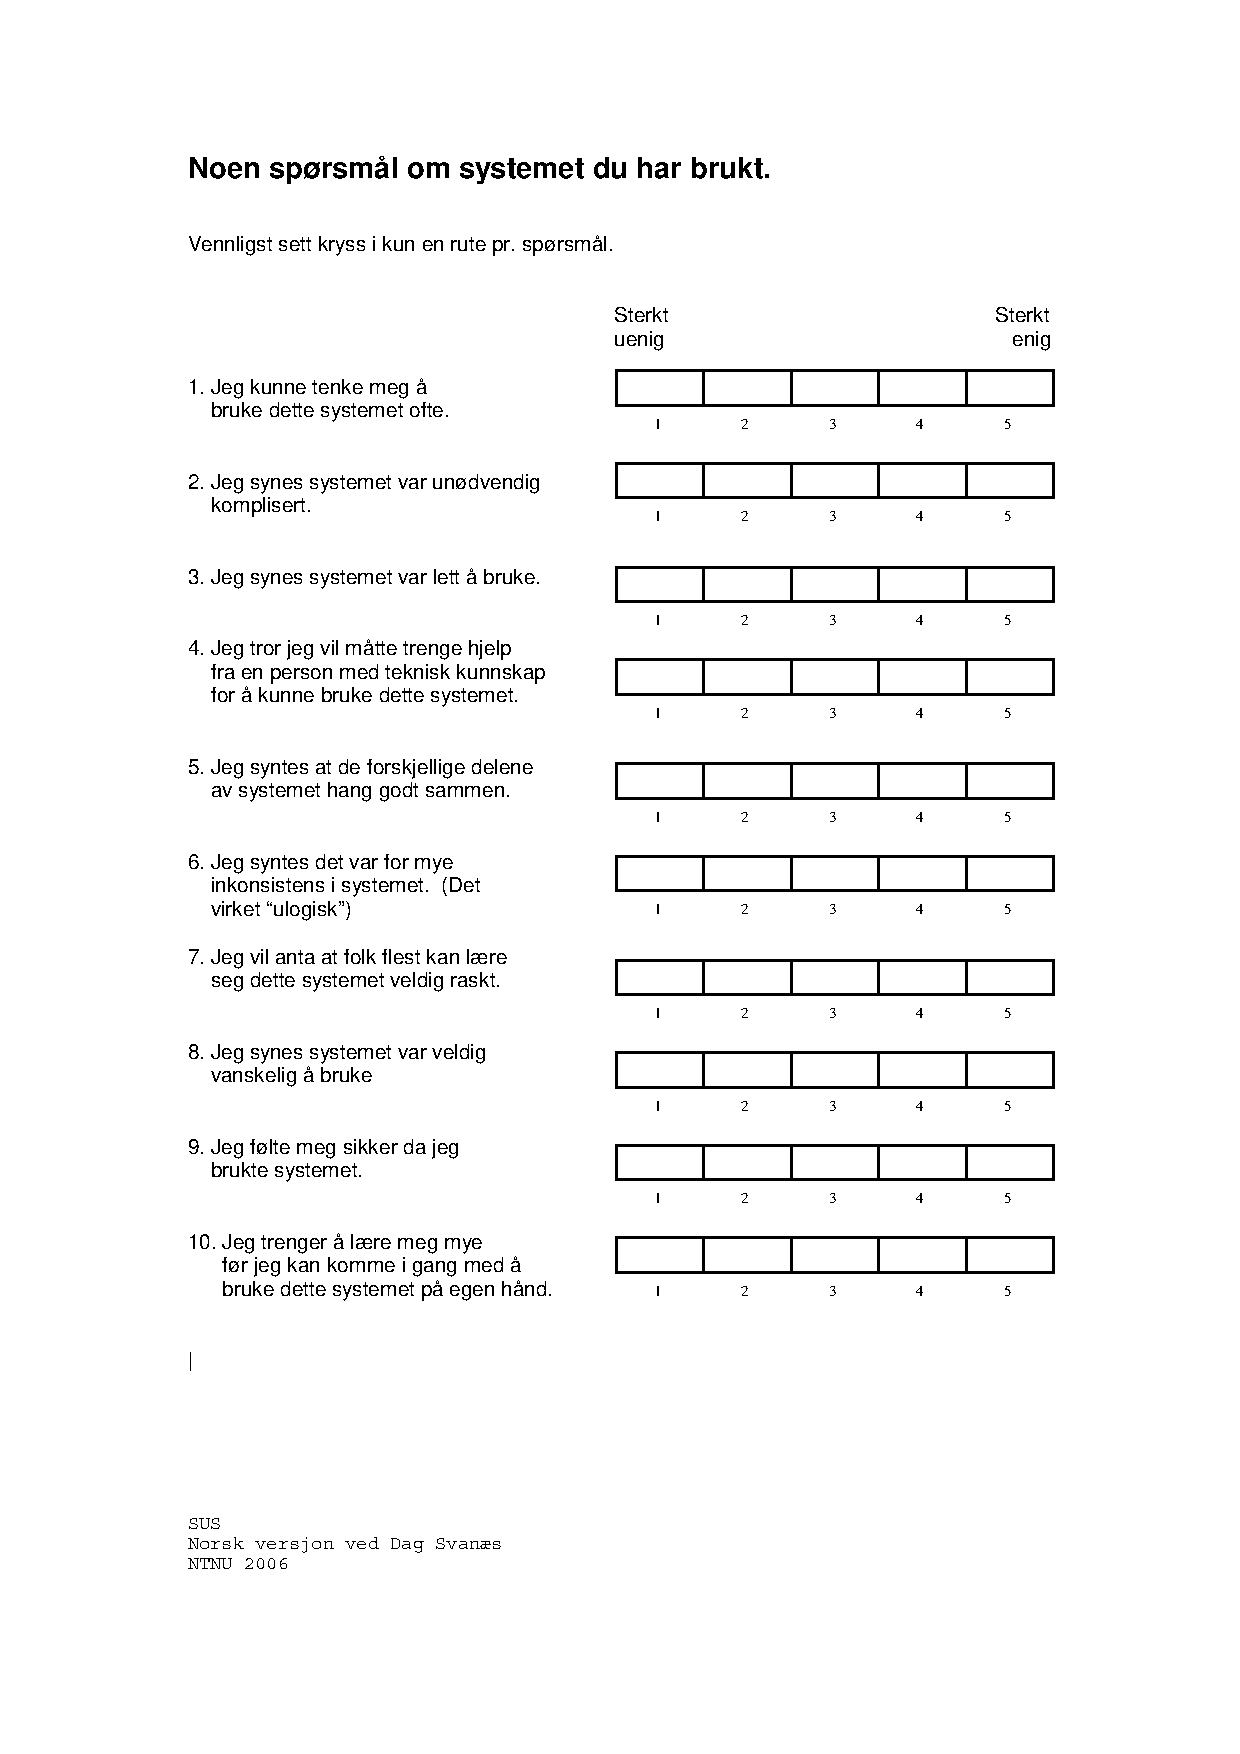
\includepdf{Appendices/susnorsk.pdf}	% Appendix Title

\chapter{Further Work}
\label{app:furtherWork}
This chapter gives an overview of some of the ideas both the customer and the developers had for further development of the application. This includes a description of further development, analysis of the user groups and work towards NAAF and the health department.
The main part of the work to be done after the end of this project is connected to requirements that has been taken out of this project due to limitation of time and resources. Other issues remaining is connected to the security and privacy of the patient's treatment log and storing sensitive information.
Section \ref{sec:frcompleted} lists the overall requirements that have not been implemented during the project. These requirements has either been requested early in the process of have been brought up during discussions and meetings with the stakeholders. 


% Here goes the major potential improvements such as privacy/security, rewardsystem and connection
\section{Improvements}
\label{sec:Improvements}
The following sections describes the ideas we had for future improvements to the applications. It is parted into subsections for improvements in the fields of database records, the reward system, the distraction and the web application.

%\input{FurtherWork/WebAccess}
%\input{FurtherWork/SecurityAndPrivacy}

\subsection{Rewardsystem}
The children's application (CAPP) is all about changing the children's view of medication to something positive. It shall be a motivation for the children to take their medication. It is therefore an important task to entertain them and give them some form of reward when they take their medication. As for now, we have given stars to the child after completed medication. The stars are in a treasure chest where the child can see how many stars he or she has. This is a simple reward, but worked fairly well during the user tests. However, it may be boring over time. 

The initial idea was to have a shop where the children could buy clothes and other items to their avatar. The stars earned from finishing treatments would serve as credits in the shop. This was not implemented due to time restrictions. It is also possible to take this to the real world, e.g. that the child gets a lollipop for every 10th star, but this would have to be supervised by the parents. 
 

There is an endless line of opportunities for this reward system, and we chose the simplest implementation, so we would have something to test. 

\subsection{Distraction sequence for children}
During our workshop, we came up with a lot of ideas for distractions for the children. These would range from simple animation sequences, like what we decided to implement, to more complex 
things like games that would not require a lot of movement and could therefore help during longer treatments. 

The distraction sequence is one of the fields were we feel it has more or less never ending possibilities for improvement, and as more research into what children finds distracting, but not to the point 
where they can't take their medicine, this distraction sequence can be evolved.


\subsection{User testing of the guardian application}
GAPP has not yet been user tested on actual parents of asthmatic children. This has to be done to get an understanding of how they interact with the system, and to get knowledge about what they think of an application of this type. This is a system to make it easier for the guardians to give their children medications. While it is important that the children likes the system, it is also important that the parents feel it helps them give their children their medicines, without it being a big time waster.

\subsection{Web application}
There is a possibility of making this application as a web application, as a whole. By extracting the functionality and running it on a web service it would make it easier for people to use it across platforms. Done right, it may run on all devices with an internet connection. This may also give an easier integration with external information such as air pollution forecast, pollen forecast, temperatures, etc. Since our application is written in Java, using Android SDK, it will not run on an internet server as is. Making a web application will require an almost complete refactoring of the source code.

 
\subsection{Support for more children}
Currently, the application only use one child, but there are implemented support for using more children. Each child has its own id (childId), and support for more children can be implemented without much change of the existing code. There should also be concidered using accounts for the guardians connected to the children, in case of the guardians having more than one asthmatic child. 
  

% Here goes the minor ideas and improvements for further work
\section{Ideas and minor improvements}


\begin{description}

\item[Webinterface] The doctors may prefer to set up the users medication plans through a web interface on their computers. This part may be integrated into existing systems. 

\item[Other devices] The application are fitted for a phone running the Android operating system. For the future it should also be scalable to tablets. There may be more interesting for a child to work on a tablet than a phone. There will also be much more space for content. This extra space gives greater potential of the reward system. It should also be available on other operating systems than Android, e.g. iOS or Windows Phone. This will improve the availability for the users, not limiting them to Android phones. 

\item[Overall graphical design] The priorities have been to make the major functionality work. We have used lots of time making the applications understandable and easy to use, but there is still a great potential in making the applications interaction design better. 

\item[Personalize the system] The application may be more personalized. E.g. "It's time to take medication" could be "It's time to take medication, Eric". By involving the users name more in the system, they may feel more appreciated. 

\item[Integration of external elements] The distraction part of the application may be integrated with a story or other external elements. I. eg. a story where the children will need to take medicine in order to get the next part of the story.

\end{description}


 % Further Work on CAPP/GAPP/KAPP

\chapter{Questionnaire. Demographics}
\label{app:questionnaire}

Vennligst besvar spørsmåle under, f\o r vi begynner testen.
\begin{center}
	\begin{tabular}{ | p{10.0cm} |}
	\hline
	\textbf{Kj\o nn} \\[5ex] \hline
	\textbf{Alder} \\[5ex] \hline
	\textbf{Utdanning} \\[5ex] \hline
	\textbf{Yrke} \\[5ex] \hline
	\end{tabular}
\end{center} % Appendix Title

\chapter{Interview Conducted Before Usability Testing}
\label{app:interviews-before-usability-testing}


\begin{center}
	\begin{tabular}{ | p{13.5cm} | }
		\hline
		\textbf{Experience with computers} \\[5ex] \hline
		\textbf{Access to internet} \\[5ex] \hline
		\textbf{Time spent online per day} \\[5ex] \hline
		\textbf{Has a smartphone} \\[5ex] \hline
		\textbf{SMS Usage} \\[5ex] \hline
		\textbf{Has facebook account} \\[5ex] \hline
		\textbf{Uses electronic reminders (calendar, to-do list etc)} \\ [5ex] \hline
	\end{tabular}
\end{center}
 % Appendix Title

\chapter{Draft for Interview Conducted after Usability Test}
\label{app:interviewafter}

After each usability test, we asked some questions to the test users, in order to make sure we collected as much feedback as possible. The questions asked to adult users and child users differed, and are listed below.

\paragraph{Questions Asked to Adult Test Users}

\begin{center}
	\begin{tabular}{ | p{5.0cm} | p{8.0cm} | }
	\hline
	\textbf{Do you have any thoughts or comments on how the test went?} & \\[5ex]  \hline
	\textbf{Where there any aspects of the test that you found difficult?} & \\[5ex] \hline
	\textbf{Why was it difficult?} & \\[5ex]  \hline
	\textbf{Have you used any similar application(s) earlier?} & \\[5ex] \hline
	\textbf{Any other comments/ideas/thoughts we should take notice of} & \\[5ex] \hline
	\end{tabular}
\end{center}


\paragraph{Questions Asked to Child Test Users}

\begin{center}
	\begin{tabular}{ | p{5.0cm} | p{8.0cm} | }
	\hline
	\textbf{Which method did you prefer with or without \ab{}?} & \\[5ex] \hline
	\textbf{Which method did you prefer? \app{} or \ab{}?} & \\[5ex] \hline
	\textbf{Do you want to play with \app{} or \ab{} one more time?} & \\[5ex] \hline
	\end{tabular}
\end{center}

\chapter{Scenario and tasks}
\label{app:scenarioandtasks}

Du er verge til et barn p\r{a}  4 \aa r. Dere har nylig v\ae rt hos en lege med spesialkompetanse p\r{a} barnesykdommer.
Barnet har f\r{a}tt diagnostisert astma. For \r{a} enklere holde orden p\r{a} at medisinene blir tatt til riktig tid, p\r{a} riktig m\r{a}te, 
har du lastet ned applikasjonen [SETT INN APPNAVN]. Systemet har ikke behov for at du registrerer navn eller lignende, 
for du \o nsker ikke at slik informasjon kommer på avveie. For at du best mulig skal kunne benytte deg av [APPNAVN], er det
n\o dvendig at du gjennomf\o rer noen oppgaver.

\paragraph{Oppgave 1:}
Du skal sette opp en medisineringsplan i henhold til anbefaling fra legen. For enkelhets skyld skal du kun endre
medisineringsplanen for barnet n\r{a}r det er helt friskt. Legg til en varsel for ``Flutide'' kl 13:37 og en varsel for ``Seretide'' kl 18:30.
Velg deretter å f\o lge denne medisineringsplanen.


\paragraph{Oppgave 2:}
Barnet ditt tok allerede en dose med medisin da dere var hos legen. Du \o nsker å starte loggf\o ringen med en gang. Etterrigstrer bruk
av Seretide kl 12:51 i dag.


\paragraph{Oppgave 3:}
Du \o nsker \r{a} motivere barnet ditt til å ta medisinene sine uten at det skal bli en krangel hver gang.
Lag en premie barnet ditt kan f\r{a} dersom hun/han har fulgt medisineringsplanen sin.
Som premiebilde kan du ta et bilde med kameraet p\a telefonen, og premietekst og antall stjerner velger du selv.


\paragraph{Oppgave 4:}
Se hvordan barnet ditt ligger an i forhold til m\r{a}let du satte i forrige oppgave?


\paragraph{Oppgave 5:}
Det er nå g\r{a}tt to uker, og du \o nsker å se hvordan du og ditt barn har fulgt medisineringsplanen. 
Let gjennom loggen for \r{a} se om dere har gjort jobben på en god nok m\r{a}te.



Du har n\r{a} gjennomf\o rt testen. Vennligst fyll inn skjemaene for \r{a} forklare hvordan du oppfattet bruken av applikasjonen.

\end{document}
 % Appendix Title

\chapter{AsthmaBuddy Manual}
\label{app:asthmabuddy_manual}

The following Appendix works as a user manual for AsthmaBuddy.

\section{Introduction}
The source code is specifically written to be run on a \rpi{}. As such, the program WILL NOT work on other computers.

\subsection{Dependencies}
\label{sec:dependencies} 
We have used a couple of frameworks in order to make the development process easier. Downloading and placing them in the correct folder is important in order to compile and run the application. 

\paragraph{Java}
As of September 2013, all \rpi{}s are shipped with Java by default. If your version of \rpi{} was bought before this, Java can be downloaded and installed through this command: 

\code{sudo apt-get update \&\& sudo apt-get install oracle-java7-jdk}

\paragraph{Pi4J}
Pi4J can be downloaded from the following URL: \url{http://pi4j.com}. To install it, simply follow the installation guide at the same page\fnurl{Pi4J Installation guide}{http://pi4j.com/install.html}. 

\paragraph{Google Gson}
Google's Gson can be downloaded from the following URL: \url{https://code.google.com/p/google-gson/downloads/list}. Put it in the folder 

\code{/home/pi/Downloads/} 

The path to gson-2.2.4.jar should be:

\code{/home/pi/Downloads/google-gson-2.2.4/gson-2.2.4.jar}.

\paragraph{JLayer}
JLayer can be downloaded the following URL: \url{http://www.javazoom.net/javalayer/javalayer.html}. Put the file \code{jl1.0.1.jar} in the folder 

\code{/home/pi/jlayer/JLayer1.0.1/}, 

which should make the path to the file:

 \code{/home/pi/jlayer/JLayer1.0.1/jl1.0.1.jar}.  

\paragraph{Joda Time}
Joda Time can be downloaded from the following URL: \url{http://www.joda.org/joda-time/}. Put the file \code{joda-time-2.3.jar} in the folder 

\code{/home/pi/Downloads/joda-time-2.3},

which should make the path to the file:

 \code{/home/pi/Downloads/joda-time-2.3/joda-time-2.3.jar}. 

\paragraph{Node.js}
Node.js can be downloaded from the following URL: \url{http://nodejs.org/}. Finding the source code for our Node.js server is found in Section \ref{sec:sourcecode}

\section{GPIO setup}
In order for \ab{} to work properly, you need to use an RGB LED diode, which is connected to the \rpi{} through the GPIO pins. This section will elaborate on the details of this process. 

Figure \ref{fig:rgb-led} shows the RGB LED-diode we used to emit light signals. As you can see, there are four pins: Blue (1), Ground(2), Green(3) and Red(4). Pins 1,3 and 4 are connected to a 220 Ohm Resistor. Figure \ref{fig:rpigpio} shows an overview of the available Gpio ports.  Table \ref{tab:wiringgpio} shows how the pins are then wired to the \rpi{}. 

\begin{figure}
	\begin{minipage}[t]{0.4\linewidth}
		\centering
			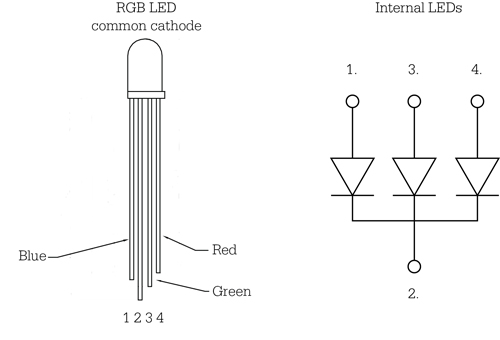
\includegraphics[width=0.30\paperwidth]{Pictures/rgb_led_diagram.jpg}
		\caption{RGB LED diagram.}
		\caption*{Image source: Purdue University \url{http://courses.cs.purdue.edu/cs25000:lab3}}
		\label{fig:rgb-led}
	\end{minipage}
	\hspace{1cm}
	\begin{minipage}[t]{0.4\linewidth}
		\centering
			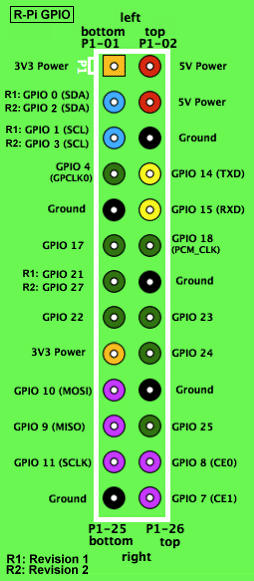
\includegraphics[width=0.20\paperwidth]{Pictures/GPIOs.png}
		\caption{\rpi{} GPIO.}
		\caption*{Image source: elinux.org \url{http://elinux.org/File:GPIOs.png}}
		\label{fig:rpigpio}
	\end{minipage}
\end{figure}

\begin{table}[H]
\centering
\begin{tabular}{|p{3.0cm}| p{3.0cm}|}
	\hline
	\textbf{LED Pin} & \textbf{Wired to GPIO port}\\
	\hline
	Blue (1) & GPIO 17\\
	\hline
	Ground (2) & Ground\\
	\hline
	Green (3) & GPIO 18\\
	\hline
	Red (4) & GPIO 21/27 (Revision 1/Revision 2)\\
	\hline
\end{tabular}
\caption{Wiring LED pins to GPIO}
\label{tab:wiringgpio}
\end{table}

\section{RFID reader}
We used the Sparkfun ID-12LA RFID-reader. This was connected through the bottom USB port on the \rpi{}. 
The application needs the port name of the USB reader. This can be found by the following command: 

\code{ls /dev | grep USB}

If the output is not equal to \code{/dev/ttyUSB0}, you can insert your name in the variable \code{comPort} in the file \code{src/com/blopp/pi/readers/RFIDReader.java}. 
 
\section{Source code}
\label{sec:sourcecode}
[TODO: Wait for clarification from Pieter, Ole and Elin]
[TODO: Remember the node server]


\section{Running AsthmaBuddy}

\subsection{Compiling}
If the guide in \ref{sec:dependencies} was followed carefully enough, the program can be compiled by running:

\code{./src/compile.sh}

Alternatively, you may extract the exact command from \code{compile.sh}, and run it directly from the terminal window. 

\subsection{Running}
The program can run by using the following script:

\code{./src/v2.sh}

Alternatively, you may extract the exact command from \code{v2.sh}, and run it directly from the terminal window. 

\paragraph{Parameters}

Once the program is running, it checks for alarms stored for the user. 

Once the message \emph{``Did not find any alarms''} appears, you can type in parameters on this format: \emph{CN}. 

C is the color of the medicine that is to be taken. C $\in \{ b = Blue, o = Orange, p = Purple \}$.

N is the interaction method you want to use. N $\in \{ 0, 1, 3, 4, 6, 9\}$. The interaction methods provided are summarized in Table \ref{tab:interactionmethodsguide}.

An example on a valid input is:

\code{b1}

\begin{table}[H]
\begin{tabular}{|p{3.0cm} | p{7.0cm}|}
\hline
\textbf{N} & \textbf{Interaction method} \\
\hline
0 & \emph{Clap your hands} \\
\hline
1 & \emph{Variation of those provided in this table} \\
\hline
3 & \emph{Hold \ab{}'s hand to proceed} \\
\hline
4 & \emph{Hold your card against \ab{}'s stomach}\\
\hline
6 & \emph{Give an high five} \\
\hline
9 & \emph{Press \ab{}'s stomach} \\
\hline
\end{tabular}
\caption{Guide for interactions in \ab{}.}
\label{tab:interactionmethodsguide}
\end{table}

After this, you can press \emph{Enter} every time the user has interacted with \ab{}, and the windows says \emph{Ready for User Input}. 

\chapter{Asthma Traffic Light System}
\label{chp:traffic-light}
\begin{figure}[H]
	\centering
	\includegraphics[scale=0.50]{Appendices/KapiolaniEDAsthmaActionPlan.pdf}
\end{figure}


\chapter{AsthmAPP Manuscript}
\label{chp:anuscript} %Hoho
During a medication process, AsthmAPP speaks to a child. The following is a breakdown on the manuscript the applications follow.
\begin{enumerate}
  \item Hei, jeg heter Blipp. N\r{a} er det p\r{a} tide \r{a} ta pustemedisin. Trykk p\r{a} hodet mitt, s\r{a} forteller jeg deg mer. \emph{Hi, my name is Blipp. It's time to take the breathing medicine. Press my head, and I'll tell you more.}
  \item Hent den C medisinen og masken du puster i, og trykk p\r{a} hodet mitt n\r{a}r du har hentet dem. \emph{Get the C medicine and the mask you breath in, then press my head when you have fetched them.}
  \item Rist den C medisinen. Trykk p\r{a} hodet n\r{a}r du er klar. \emph{Shake the blue medicine. Press my head when you are ready}
  \item Av den C medisinen skal du ta 1 puff. Sett p\r{a} deg masken og gj\o r deg klar. Trykk p\r{a} hodet mitt, s\r{a} teller jeg mens du puster inn og ut. \emph{You are going to take 1 spray of the C medicine. Put on your mask and get ready. Press my head, and I'll count when you breathe in and out.} 
  \item N\r{a}r jeg sier i fra, skal du trykke 1 gang. Trykk p\r{a} hodet mitt, s\r{a} begynner jeg \r{a} telle. \emph{Upon signal, press the medicine one time. Press my head, and I'll start counting. }
  \item 1, 2, 3, 4, 5, 6, 7, 8, 9, 10.
  \item N\r{a} var du flink. \emph{You did great}
  \item Som bel\o nning f\r{a}r du N stjerner i skattekista di. \emph{As a reward, you'll get S stars in your treasure chest.}
\end{enumerate}

The above script has the following properties:

C $\in \{ Blue, Orange, Purple \}$


S $\in \{ 1, 3, 5 \}$ 


\chapter{Constraints}
\label{chp:securityrequirements}

By law, we have some constraints in order to proceed start usability testing. This Appenix cover these. 

\section{The Health Register Act}
\label{sec:helseregisterloven}

Norway has specific laws for storing of medical information. The most significant law is ``The Health Register Act\footnote{Lov om helseregistre og behandling av helseopplysninger}''\cite{helseregisterloven}. This law regulates who is allowed to store health records and how they store the records. 

The most significant consequences is that the information has to be stored on servers on Norwegian soil. This eliminates the option of using cloud-based services such as Amazon EC2, Windows Azure or Google App Engine. 

In addition, we need permission from \emph{REK} \fnurl{https://helseforskning.etikkom.no/} in order to store medical records in the application. If the application were ever to be deployed to Google Play, we would need permission from \emph{The Data Protection Authority}, but it not required if the application is just for research purposes. Our application is still pending.

\section{Measures for Anonymization}
Pursuant to section 16 of the Health Register Act \cite{helseregisterloven} all information that may identify a person, must be encrypted, i.e. it should be impossible to find which person a specific record corresponds to by looking at a database dump.  


\lhead{\emph{Bibliography}}  % Change the left side page header to "Bibliography"
\bibliographystyle{unsrtnat}  % Use the "unsrtnat" BibTeX style for formatting the Bibliography
\bibliography{Bibliography}  % The references (bibliography) information are stored in the file named "Bibliography.bib"

\addtocontents{toc}{\vspace{2em}}  % Add a gap in the Contents, for aesthetics
\backmatter

%% ----------------------------------------------------------------

\end{document} 